% This LaTeX was auto-generated from MATLAB code.
% To make changes, update the MATLAB code and export to LaTeX again.

\documentclass{article}

\usepackage[utf8]{inputenc}
\usepackage[T1]{fontenc}
\usepackage{lmodern}
\usepackage{graphicx}
\usepackage{color}
\usepackage{hyperref}
\usepackage{amsmath}
\usepackage{amsfonts}
\usepackage{epstopdf}
\usepackage[table]{xcolor}
\usepackage{matlab}
\usepackage{ctex}
\usepackage[paperheight=845pt,paperwidth=597pt,top=72pt,bottom=72pt,right=72pt,left=72pt,heightrounded]{geometry}

\sloppy
\epstopdfsetup{outdir=./}
\graphicspath{ {./HodgkinHuxley_media/} }

\matlabhastoc

\begin{document}

\label{TMP_1a1d}
\vspace{1em}

\label{TMP_706a}

\vspace{1em}
\matlabtableofcontents{目录}
\label{TMP_691a}
\vspace{1em}

\label{TMP_1eca}
\vspace{1em}

\label{TMP_22a2}
\matlabtitle{课题 1 : 可激发系统的模拟: Hodgkin-Huxley 神经元模型}


\vspace{1em}
\label{TMP_4450}
\matlabheading{可激发系统}


\vspace{1em}
\begin{par}
\begin{flushleft}
 可激发介质/系统 (excitable medium/system): 简言之就是具有 “可激励性”的介质, 也叫激励介质  
\end{flushleft}
\end{par}

\begin{par}
\begin{flushleft}
“可激励性”所对应的英文单词是“excitability”. 这个词在不同 的学科里有不同的译法: 物理学中叫可激发性, 医学中叫兴奋性、 敏感性, 生理学中叫刺激反应性 这里所指的“可激励性”是当介质 受到小扰动时, 介质很快恢复到平衡态 (静态); 但当扰动超过某一 阈值时, 介质将有一个快速又陡峭的响应, 呈现激发状态  
\end{flushleft}
\end{par}

\label{TMP_4676}
\matlabheading{神经元}

\begin{par}
\begin{flushleft}
大脑中神经元数目巨大 \textasciitilde{}10\textasciicircum{}11  
\end{flushleft}
\end{par}

\begin{par}
\begin{flushleft}
神经元形状及其多样  
\end{flushleft}
\end{par}


\vspace{1em}
\begin{par}
\begin{flushleft}
图中的标注及其翻译:
\end{flushleft}
\end{par}

\begin{par}
\begin{flushleft}
Soma :胞体
\end{flushleft}
\end{par}

\begin{par}
$$\textrm{Neurites}\textrm{:神经突}\left\lbrace \begin{array}{ll}
\textrm{Dendrites}\textrm{树突} & \\
\textrm{Axon}\textrm{:轴突} & 
\end{array}\right.$$
\end{par}

\label{TMP_3d9c}
\matlabheading{神经元的可激发性}

\begin{par}
\begin{flushleft}
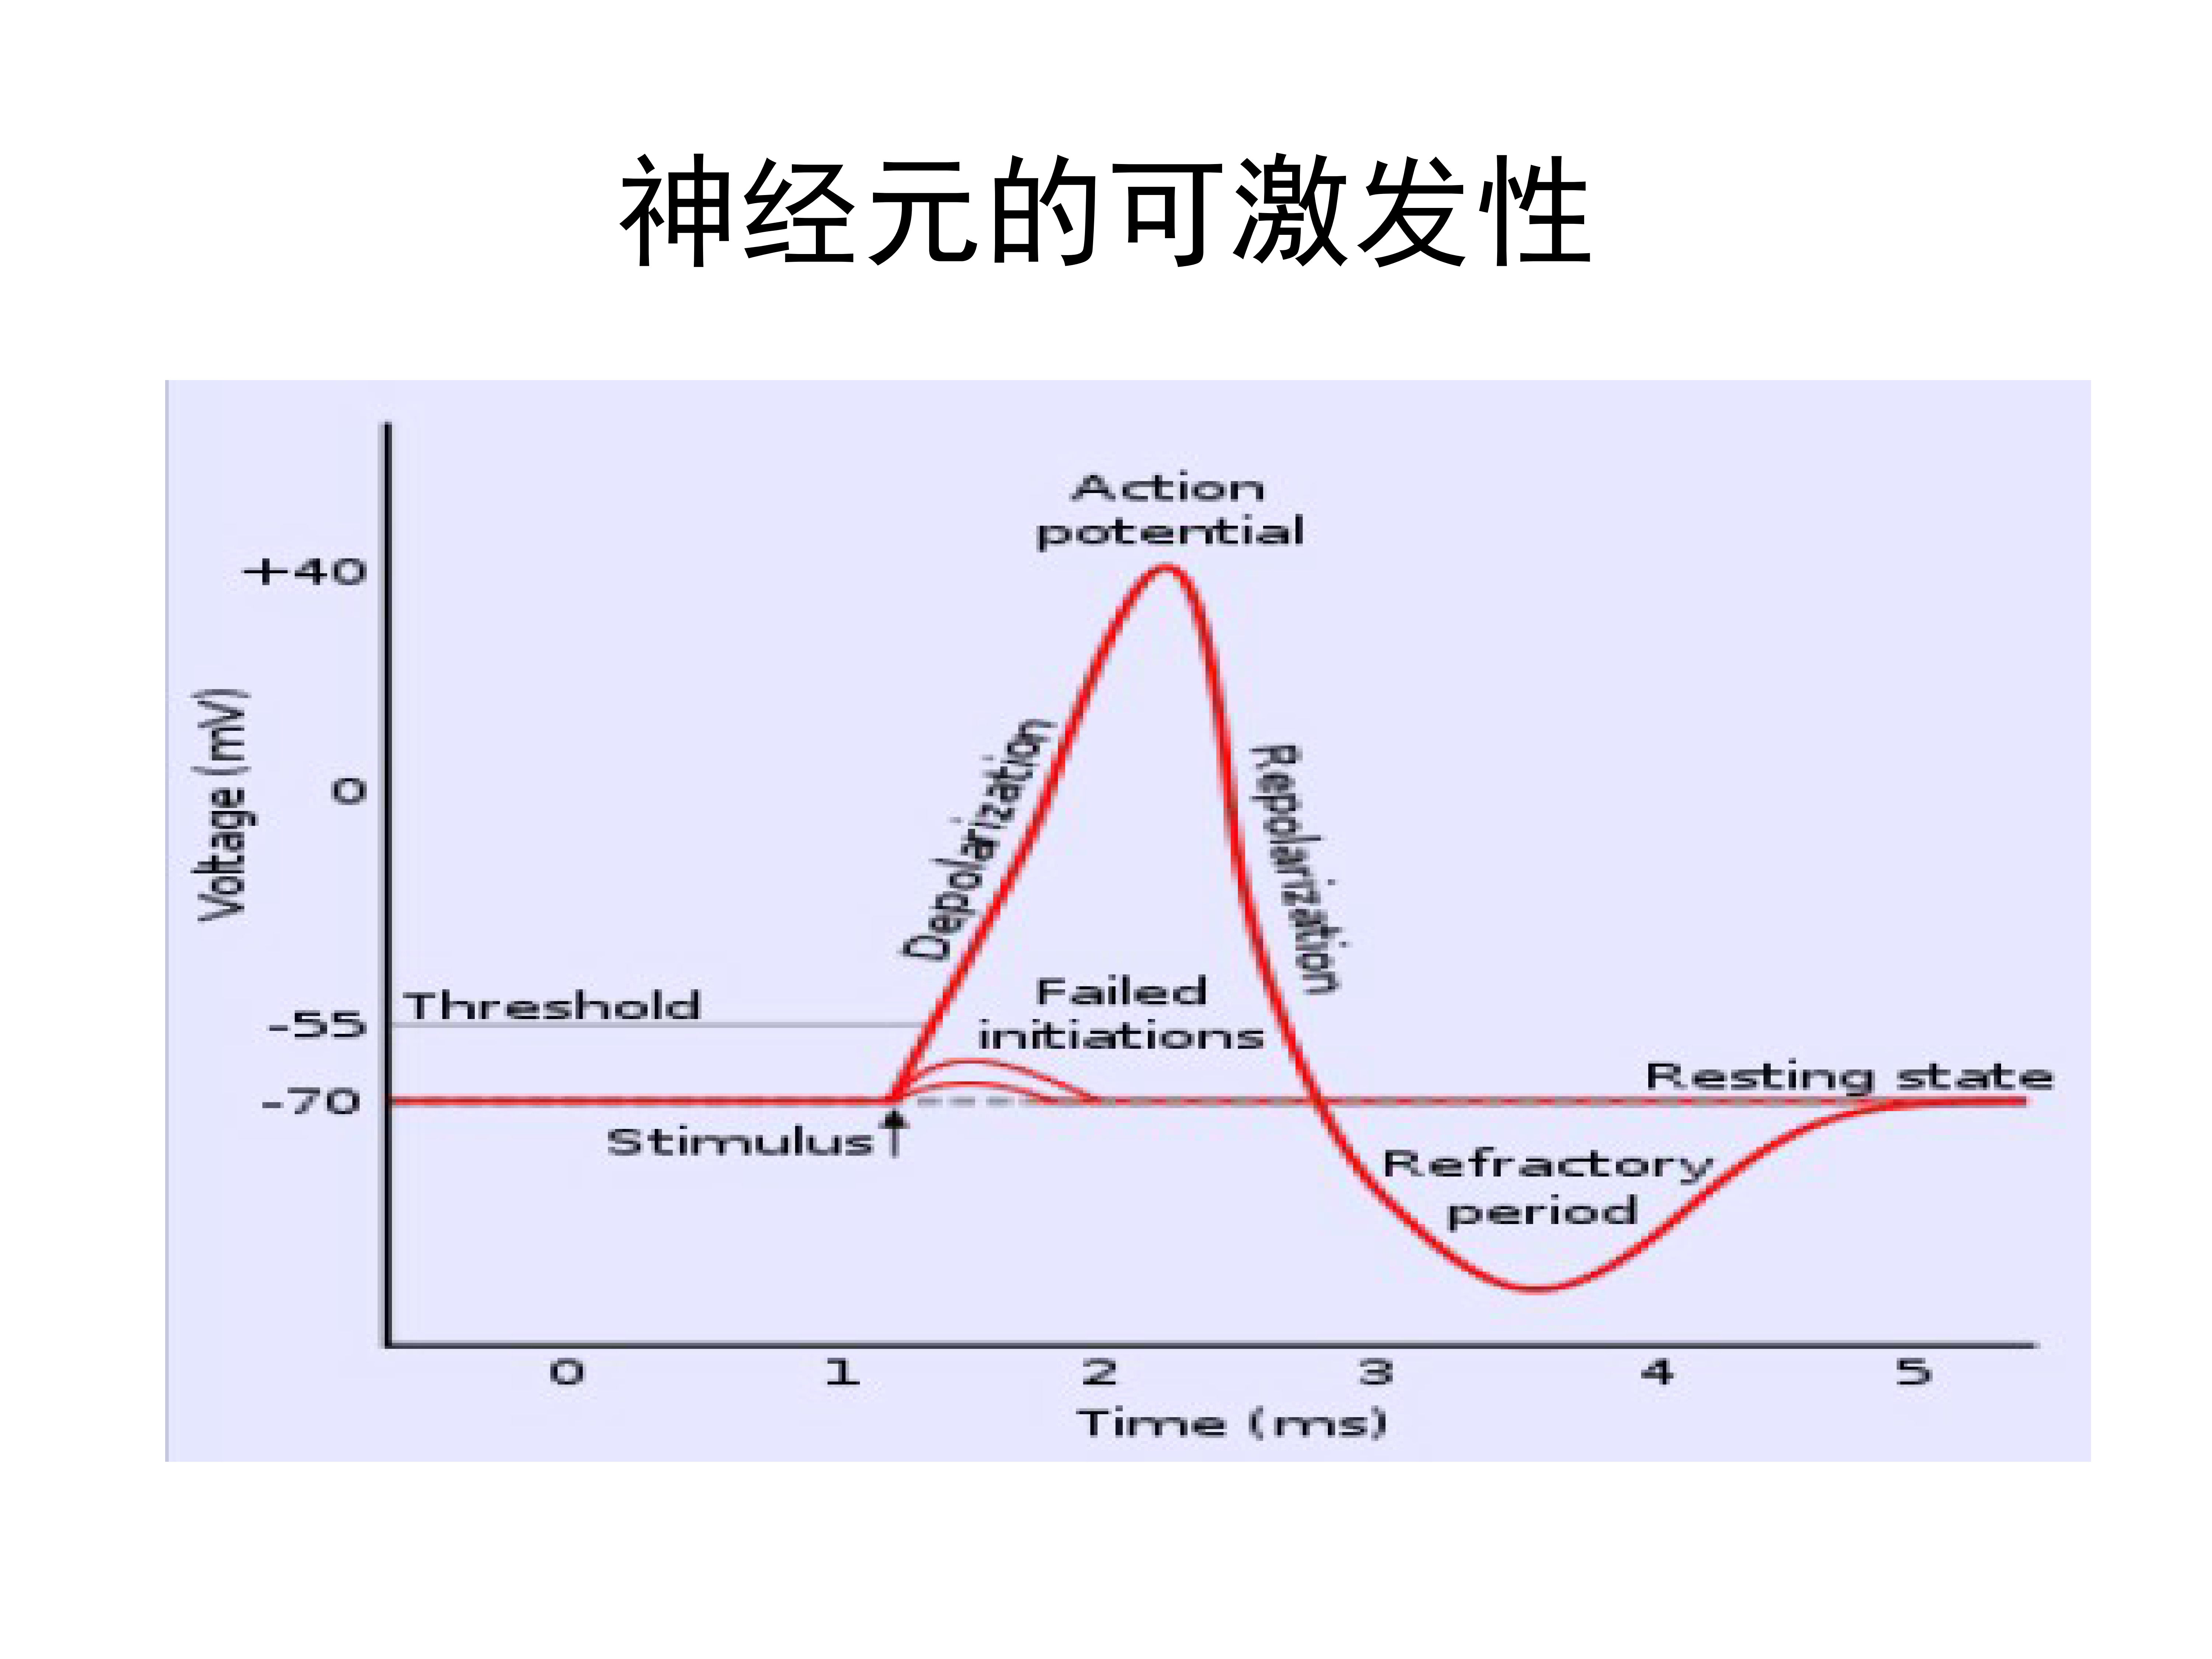
\includegraphics[width=\maxwidth{28.19869543401907em}]{image_0}
\end{flushleft}
\end{par}

\begin{par}
\begin{flushleft}
图中的标注及其翻译:
\end{flushleft}
\end{par}

\begin{par}
\begin{flushleft}
  Action potential :动作电势
\end{flushleft}
\end{par}

\begin{par}
\begin{flushleft}
  Depolarization :去极化
\end{flushleft}
\end{par}

\begin{par}
\begin{flushleft}
  Repolarization :复极化
\end{flushleft}
\end{par}

\begin{par}
\begin{flushleft}
  Failed initiations :失败的启动
\end{flushleft}
\end{par}

\begin{par}
\begin{flushleft}
  Threshold :阈值
\end{flushleft}
\end{par}

\begin{par}
\begin{flushleft}
  Resting state :静息态
\end{flushleft}
\end{par}

\begin{par}
\begin{flushleft}
  Stimulus :刺激
\end{flushleft}
\end{par}

\begin{par}
\begin{flushleft}
  Refractory period 不应期
\end{flushleft}
\end{par}


\vspace{1em}
\begin{par}
\begin{flushleft}
神经元在受到刺激时膜电位随时间变化的过程,称为\textbf{动作电势} 
\end{flushleft}
\end{par}


\vspace{1em}
\begin{par}
\begin{flushleft}
\textbf{Y轴 :} 电压,单位:mV 神经元细胞膜内外的电位差  
\end{flushleft}
\end{par}

\begin{par}
\begin{flushleft}
**X轴:**时间,单位:毫秒
\end{flushleft}
\end{par}

\begin{itemize}
\setlength{\itemsep}{-1ex}
   \item{\begin{flushleft} \textbf{三个电位水平 Potential Levels:} \end{flushleft}}
   \item{\begin{flushleft} \textbf{Resting state (静息态):} 约 -70 mV 神经元在未受刺激时的稳定电位 \end{flushleft}}
   \item{\begin{flushleft} \textbf{Threshold (阈值):} 约 -55 mV 临界电位 \end{flushleft}}
   \item{\begin{flushleft} \textbf{峰值:} 约 +40 mV 动作电势达到的最高电位 \end{flushleft}}
   \item{\begin{flushleft} \textbf{事件:} \end{flushleft}}
\end{itemize}

\begin{enumerate}
\setlength{\itemsep}{-1ex}
   \item{\begin{flushleft} \textbf{Stimulus (刺激):} 在 1 ms 稍过一点的位置,一个外部刺激被施加 \end{flushleft}}
   \item{\begin{flushleft} \textbf{Failed initiations (失败的启动):} 图中阈值下方的小波形  这表示刺激强度太弱,没有使膜电位达到 -55 mV 的阈值,因此无法触发一个完整的动作电势,电位很快就回落到静息态 \end{flushleft}}
   \item{\begin{flushleft} \textbf{Depolarization (去极化):} 当一个足够强的刺激使膜电位达到阈值 (-55 mV) 后,膜电位开始急剧上升,从负值变为正值,一直达到 +40 mV 的峰值 \end{flushleft}}
   \item{\begin{flushleft} \textbf{Action potential (动作电势):} 整个快速的电位“尖峰”(从去极化开始到复极化结束)被称为动作电势  图中的标签也特指其峰值 \end{flushleft}}
   \item{\begin{flushleft} \textbf{Repolarization (复极化):} 达到峰值后,膜电位迅速下降,从 +40 mV 降回负值 \end{flushleft}}
   \item{\begin{flushleft} \textbf{Refractory period (不应期):} 膜电位在复极化后,会短暂地降到比静息态(-70 mV)更低的水平  在这个时期,神经元对新的刺激反应能力降低(或完全不反应)  之后,电位会逐渐恢复到 -70 mV 的静息态   \end{flushleft}}
\end{enumerate}

\label{TMP_3d49}
\matlabheading{动作电势的特性}

\begin{par}
\begin{flushleft}
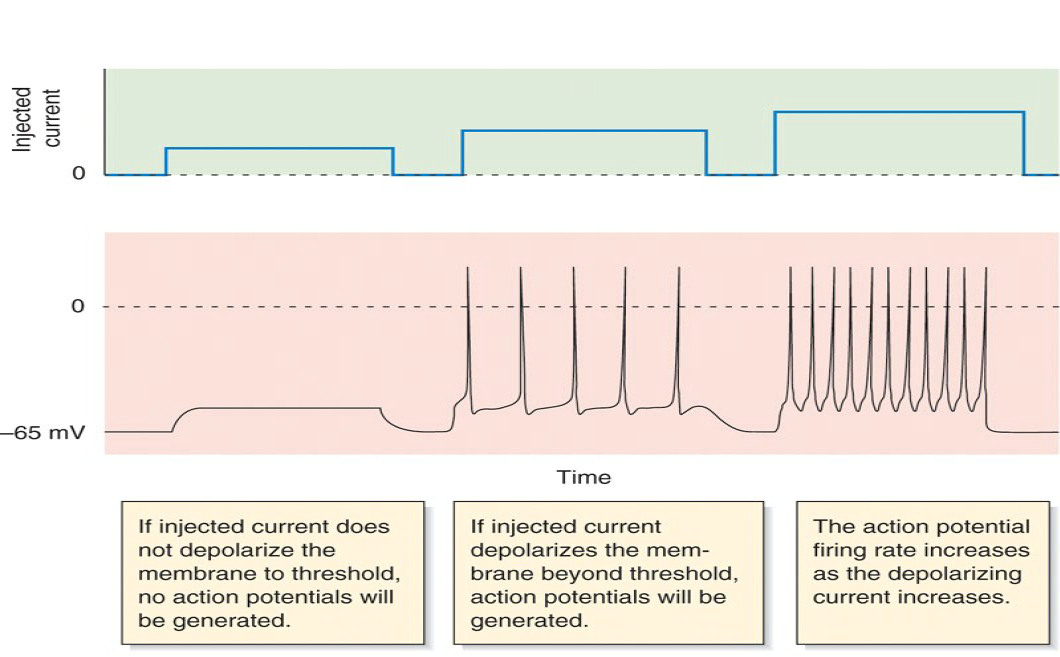
\includegraphics[width=\maxwidth{36.82890115403914em}]{image_1}
\end{flushleft}
\end{par}


\vspace{1em}
\begin{par}
\begin{flushleft}
  Injected current :注入电流
\end{flushleft}
\end{par}

\begin{par}
\begin{flushleft}
1.  If injected current does not depolarize the membrane to threshold, no action potentials will be generated.
\end{flushleft}
\end{par}

\begin{par}
\begin{flushleft}
    如果注入的电流没有使细胞膜去极化到阈值,则不会产生动作电势  
\end{flushleft}
\end{par}

\begin{par}
\begin{flushleft}
2.  If injected current depolarizes the membrane beyond threshold, action potentials will be generated.
\end{flushleft}
\end{par}

\begin{par}
\begin{flushleft}
    如果注入的电流使细胞膜去极化超过阈值,则会产生动作电势  
\end{flushleft}
\end{par}

\begin{par}
\begin{flushleft}
3.  The action potential firing rate increases as the depolarizing current increases.
\end{flushleft}
\end{par}

\begin{par}
\begin{flushleft}
    随着去极化电流的增加,动作电势的发放频率增加 
\end{flushleft}
\end{par}


\vspace{1em}
\label{TMP_821d}
\matlabheading{神经元的数学建模}


\vspace{1em}
\label{TMP_2041}
\matlabheadingtwo{细胞膜与离子通道}


\vspace{1em}
\begin{par}
\begin{flushleft}
  channel 通道
\end{flushleft}
\end{par}

\begin{par}
\begin{flushleft}
  pore 孔隙
\end{flushleft}
\end{par}

\begin{par}
\begin{flushleft}
  lipid bilayer 脂双层
\end{flushleft}
\end{par}


\vspace{1em}
\label{TMP_07cb}
\matlabheadingtwo{等效电路}

\begin{par}
\begin{flushleft}
等效成了三个电阻和一个电容并联,并且在每个电阻的回路串上电池,每个电迟代表了对应离子的能斯特电位,电阻则代表了离子泵的耗能
\end{flushleft}
\end{par}

\begin{par}
\begin{flushleft}
这个模型中的能量来源是电池提供的,即营养物质的摄入
\end{flushleft}
\end{par}

\label{TMP_29fc}
\matlabheadingthree{PPT上指出的公式}

\begin{par}
\begin{flushleft}
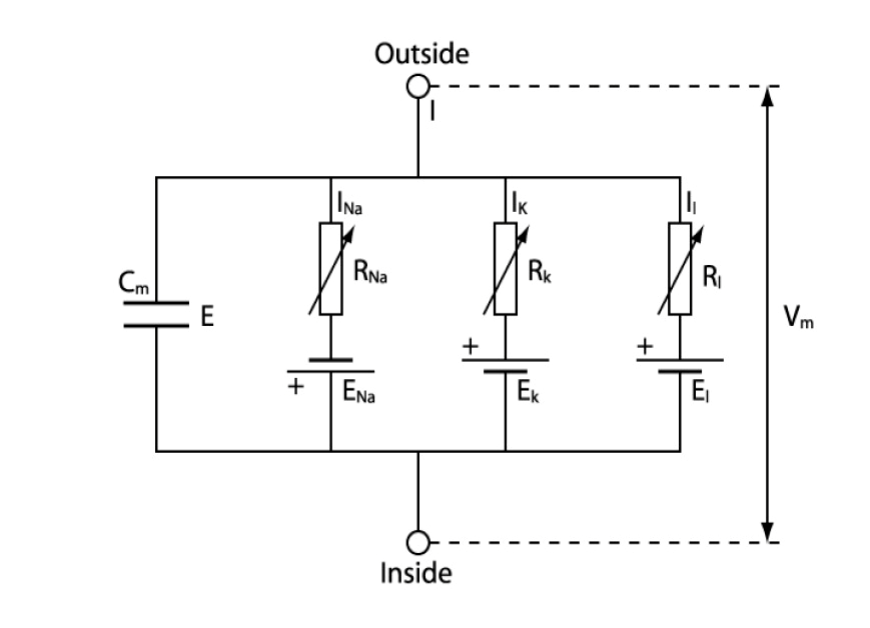
\includegraphics[width=\maxwidth{22.880080280983442em}]{image_2}
\end{flushleft}
\end{par}

\begin{par}
$$C_m \frac{dV_m }{dt}+I_{ion} =I_{ext}$$
\end{par}

\begin{par}
$$I_{ion} =\sum_k I_k =\sum_k G_k (V_m -E_k )\ldotp$$
\end{par}

\begin{par}
\begin{flushleft}
这里的$I_{ext}$ 是外部总电流,$I_{ion}$指离子电流之和
\end{flushleft}
\end{par}

\begin{par}
\begin{flushleft}
离子有三种,Na, K,还有泄露(主要是氯离子)
\end{flushleft}
\end{par}

\begin{par}
\begin{flushleft}
 $V_m$ 是指内外模的电势差,$G_k$指电导
\end{flushleft}
\end{par}

\label{TMP_1ceb}
\matlabheadingthree{PPT中给出的微分方程是}

\begin{par}
$$\left\lbrace \begin{array}{l}
C_m \frac{dV}{dt}=-g_L (V-E_L )-{\bar{g} }_{Na} m^3 h(V-E_{Na} )-{\bar{g} }_K n^4 (V-E_K )+I_{app} \\
\frac{dm}{dt}=\alpha_m (V)(1-m)-\beta_m (V)m\\
\frac{dh}{dt}=\alpha_h (V)(1-h)-\beta_h (V)h\\
\frac{dn}{dt}=\alpha_n (V)(1-n)-\beta_n (V)n
\end{array}\right.$$
\end{par}


\vspace{1em}
\begin{par}
\begin{flushleft}
HH 模型描述了动作电势的发生过程  
\end{flushleft}
\end{par}

\label{TMP_913d}
\matlabheadingthree{PPT中给出的参数是}

\begin{par}
\begin{flushleft}
电容:$C=1\mu {\textrm{F/cm}}^2$
\end{flushleft}
\end{par}


\vspace{1em}
\begin{par}
\begin{flushleft}
各离子的能斯特电位和对应的电导:
\end{flushleft}
\end{par}

\begin{par}
$$\begin{array}{lrr}
\hline
x & E_x \;\textrm{[mV]} & g_x {\;\textrm{[mS}\;\textrm{/}\;\textrm{cm}}^2 \textrm{]}\\
\hline
\textrm{Na} & 55 & 40\\
\textrm{K} & -77 & 35\\
\textrm{L} & -65 & 0.3\\
\hline
\end{array}$$
\end{par}

\begin{par}
\begin{flushleft}
对应的 alpha和beta函数:
\end{flushleft}
\end{par}

\begin{par}
$$\begin{array}{lcc}
\hline
x & \alpha_x (u/\;\textrm{mV}){\;\textrm{[ms}}^{-1} \textrm{]} & \beta_x (u/\cdot \;\textrm{mV}){\;\textrm{[ms}}^{-1} \textrm{]}\\
\hline
n & 0.02(u-25)/[1-e^{-(u-25)/9} ] & -0.002(u-25)/[1-e^{(u-25)/9} ]\\
m & 0.182(u+35)/[1-e^{-(u+35)/9} ] & -0.124(u+35)/[1-e^{(u+35)/9} ]\\
h & 0.25e^{-(u+90)/12}  & 0.25e^{(u+62)/6} /e^{(u+90)/12} \\
\hline
\end{array}$$
\end{par}


\vspace{1em}
\label{TMP_2bec}
\matlabheadingthree{文献中给出的微分方程:}


\vspace{1em}
\begin{par}
\begin{flushleft}
根据《Energy and information in Hodgkin-Huxley neurons》A. Moujahid, A. d’Anjou, and F. J. Torrealdea
\end{flushleft}
\end{par}

\begin{par}
\begin{flushleft}
突奇-赫胥黎HH模型描述了无动作电位传播的鱿鱼巨轴突,将其视为通用神经元动力学的代表,遵循以下微分方程:
\end{flushleft}
\end{par}

\begin{par}
$$\begin{array}{rcl}
C\dot{V}  & = & -i_{Na} -i_K -i_l +I,\\
\dot{m}  & = & \alpha_m (V)(1-m)-\beta_m (V)m,\\
\dot{n}  & = & \alpha_n (V)(1-n)-\beta_n (V)n,\\
\dot{h}  & = & \alpha_h (V)(1-h)-\beta_h (V)h,
\end{array}~~(1)$$
\end{par}


\vspace{1em}
\begin{par}
\begin{flushleft}
其中 $V$ 是以 $mV$ 为单位的\textbf{膜电位},$C$ 是以 $\mu F$ 为单位的\textbf{膜电容}
\end{flushleft}
\end{par}

\begin{par}
\begin{flushleft}
$I$ 是以 $\mu A/cm^2$ 为单位的\textbf{总膜电流密度}
\end{flushleft}
\end{par}

\begin{par}
\begin{flushleft}
而 $m$、$n$ 和 $h\,$ 是无量纲变量
\end{flushleft}
\end{par}

\begin{par}
\begin{flushleft}
分别表示\textbf{膜内侧钠激活分子的比例}、\textbf{膜内侧钾激活粒子的比例}
\end{flushleft}
\end{par}

\begin{par}
\begin{flushleft}
以及\textbf{膜外侧钠失活分子的比例} 。
\end{flushleft}
\end{par}


\vspace{1em}
\begin{par}
\begin{flushleft}
A. Moujahid文章中的钠、钾和泄漏 (主要是氯) 的离子电流,分别记为 $i_{Na}$、$i_K$
\end{flushleft}
\end{par}

\begin{par}
\begin{flushleft}
和 $i_l$,由下式给出:
\end{flushleft}
\end{par}


\vspace{1em}
\begin{par}
$$\begin{array}{rcl}
i_{Na}  & = & g_{Na} m^3 h(V-E_{Na} ),\\
i_K  & = & g_K n^4 (V-E_K ),\\
i_l  & = & g_l (V-E_l ),
\end{array}~~(2)$$
\end{par}


\vspace{1em}
\begin{par}
\begin{flushleft}
其中 $g_{Na}$、$g_K$ 和 $g_l$ 是各自离子通道电导的最大可能值,并且
\end{flushleft}
\end{par}

\begin{par}
\begin{flushleft}
$E_{Na}$、$E_K$ 和 $E_l$ 离子在神经元静态状态下的能斯特电位。在这
\end{flushleft}
\end{par}

\begin{par}
\begin{flushleft}
项工作中,我们给出了这些参数的标准常数值,这些值在下表中给出。
\end{flushleft}
\end{par}

\label{TMP_2019}
\matlabheadingthree{文献中给出的参数是}

\begin{par}
\begin{flushleft}
膜电容为  $C=1\mu {\textrm{F/cm}}^2$
\end{flushleft}
\end{par}

\begin{par}
\begin{flushleft}
电压标度被偏移,使得静息电位为零
\end{flushleft}
\end{par}

\begin{par}
$$\begin{array}{lrr}
\hline
x & g_x {\;\textrm{(mS/cm}}^2 \textrm{)} & E_x \;\textrm{(mV)}\\
\hline
\textrm{Na} & 120 & 115\\
\textrm{K} & 36 & -12\\
\textrm{l} & 0.3 & 10.6\\
\hline
\end{array}$$
\end{par}

\begin{par}
\begin{flushleft}
A. Moujahid文章中随时间变化的变量alpha和beta函数是
\end{flushleft}
\end{par}


\vspace{1em}
\begin{par}
$$\begin{array}{rcl}
\alpha_m (V) & = & (2.5-0.1V)/[\exp (2.5-0.1V)-1],\\
\beta_m (V) & = & 4\exp (-V/18),\\
\alpha_n (V) & = & (0.1-0.01V)/[\exp (1-0.1V)-1],\\
\beta_n (V) & = & 0.125\exp (-V/80),\\
\alpha_h (V) & = & 0.07\exp (-V/20),\\
\beta_h (V) & = & 1/[\exp (3-0.1V)+1].
\end{array}$$
\end{par}


\vspace{1em}

\label{TMP_77e2}
\matlabheading{Task1任务 1:研究不同刺激强度下神经元膜电势的变化}


\vspace{1em}

\vspace{1em}
\begin{par}
\begin{flushleft}
  请利用四阶 Rung=Kutta 算法求解 HH 方程, 并研究不同刺激强度下神经元膜电势的变化, 借此理解可激发系统的响应特性  
\end{flushleft}
\end{par}


\vspace{1em}
\begin{par}
\begin{flushleft}
脉冲刺激 或 直流刺激
\end{flushleft}
\end{par}


\vspace{1em}
\begin{par}
\begin{flushleft}
解答:
\end{flushleft}
\end{par}

\begin{par}
\begin{flushleft}
我们将分别对 脉冲刺激 或 直流刺激 使用PPT中的参数和方程 文献中对应的参数和方程 ,因此组合后结果应该有四种:
\end{flushleft}
\end{par}

\begin{par}
\begin{flushleft}
我们先复现PPT中的结果:
\end{flushleft}
\end{par}

\label{TMP_0036}
\vspace{1em}


\vspace{1em}


\vspace{1em}
\label{TMP_90d8}
\matlabheadingtwo{脉冲刺激1-使用PPT中的参数和方程}

\begin{par}
\begin{flushleft}
此时的常数为
\end{flushleft}
\end{par}

\label{TMP_6c4e}
\begin{par}
\begin{flushleft}
PPT中给出的参数是
\end{flushleft}
\end{par}

\begin{par}
\begin{flushleft}
电容:$C=1\mu {\textrm{F/cm}}^2$
\end{flushleft}
\end{par}

\begin{matlabcode}
clc;clear;
C=1;
\end{matlabcode}

\begin{par}
\begin{flushleft}
各离子的能斯特电位和对应的电导:
\end{flushleft}
\end{par}

\begin{par}
$$\begin{array}{lrr}
\hline
x & E_x \;\textrm{[mV]} & g_x {\;\textrm{[mS}\;\textrm{/}\;\textrm{cm}}^2 \textrm{]}\\
\hline
\textrm{Na} & 55 & 40\\
\textrm{K} & -77 & 35\\
\textrm{L} & -65 & 0.3\\
\hline
\end{array}$$
\end{par}

\begin{matlabcode}
E.Na=55;E.K=-77;E.L=-65;
g.Na=40;g.K=35;g.L=0.3;

% E.Na=115;E.K=-12;E.L=10.6;
% g.Na=120;g.K=36;g.L=0.3;
\end{matlabcode}

\begin{par}
\begin{flushleft}
对应的 alpha和beta函数:
\end{flushleft}
\end{par}

\begin{par}
$$\begin{array}{lcc}
\hline
x & \alpha_x (u/\;\textrm{mV}){\;\textrm{[ms}}^{-1} \textrm{]} & \beta_x (u/\cdot \;\textrm{mV}){\;\textrm{[ms}}^{-1} \textrm{]}\\
\hline
n & 0.02(u-25)/[1-e^{-(u-25)/9} ] & -0.002(u-25)/[1-e^{(u-25)/9} ]\\
m & 0.182(u+35)/[1-e^{-(u+35)/9} ] & -0.124(u+35)/[1-e^{(u+35)/9} ]\\
h & 0.25e^{-(u+90)/12}  & 0.25e^{(u+62)/6} /e^{(u+90)/12} \\
\hline
\end{array}$$
\end{par}

\begin{matlabcode}
Alpha.n=@(u) 0.02*(u-25)/(1-exp(-(u-25)/9));
Alpha.m=@(u) 0.182*(u+35)/(1-exp(-(u+35)/9));
Alpha.h=@(u) 0.25*exp(-(u+90)/12);
Beta.n=@(u) -0.002*(u-25)/(1-exp((u-25)/9));
Beta.m=@(u) -0.124*(u+35)/(1-exp((u+35)/9));
Beta.h=@(u) 0.25*exp((u+62)/6)/exp((u+90)/12);

% Alpha.n=@(u) (0.1 - 0.01.*u) ./ (exp(1 - 0.1.*u) - 1);
% Alpha.m=@(u) (2.5 - 0.1.*u) ./ (exp(2.5 - 0.1.*u) - 1);
% Alpha.h=@(u) 0.07 .* exp(-u./20);
% Beta.n=@(u) 0.125 .* exp(-u./80);
% Beta.m=@(u) 4 .* exp(-u./18);
% Beta.h=@(u) 1 ./ (exp(3 - 0.1.*u) + 1);

fs= 4000;%采样频率
T=200;%总时长(ms)
A=15;%刺激电流强度

% I_ext = @(u) 0+(20<=u & u<= 30).*A...
%     +(40<=u & u<= 50).*A/2 ...
%     +(60<=u & u<= 70).*A/4 ...
%     +(80<=u & u<= 90).*A/8 ...
%     +(100<=u & u<= 110).*A/10 ...
%     +(120<=u & u<= 130).*A/12 ...
%     +(140<=u & u<= 150).*A/14 ...
%     +(160<=u & u<= 170).*A/16 ...
%     +(180<=u & u<= 190).*A/20 ...
% ;%脉冲刺激向量
Center=(25:20:185)';%脉冲中心位置,取转置是因为要列向量
Scale=[1,1/2,1/4,1/8,1/10,1/12,1/14,1/16,1/20]';%脉冲高度
Amplitude=A*Scale;
D1=[Center,Amplitude];%用给pulstran函数,第一列脉冲中心,第二列脉冲高度
PulWidth=10;%脉冲刺激宽度为10ms
PulShap=@(t) rectpuls(t,PulWidth);%脉冲刺激函数
I_ext=@(u) pulstran(u,D1,PulShap);

Task1I2V_DC(C,E,g,Alpha,Beta, ...
    'fs',fs, ...
    'T',T, ...
    'A',A, ...
    'I_ext',I_ext);
\end{matlabcode}
\begin{matlaboutput}
此时使用的参数为:
 C: 1.0000 
g的结构体:
    Na: 40
     K: 35
     L: 0.300000000000000

E的结构体:
    Na: 55
     K: -77
     L: -65

Alpha函数的结构体:
    n: @(u)0.02*(u-25)/(1-exp(-(u-25)/9))
    m: @(u)0.182*(u+35)/(1-exp(-(u+35)/9))
    h: @(u)0.25*exp(-(u+90)/12)

Beta函数的结构体:
    n: @(u)-0.002*(u-25)/(1-exp((u-25)/9))
    m: @(u)-0.124*(u+35)/(1-exp((u+35)/9))
    h: @(u)0.25*exp((u+62)/6)/exp((u+90)/12)

外部刺激电流:
    @(u)pulstran(u,D1,PulShap)

当A=15时的外部电流刺激I-t和膜电压V-t图 
\end{matlaboutput}
\begin{center}
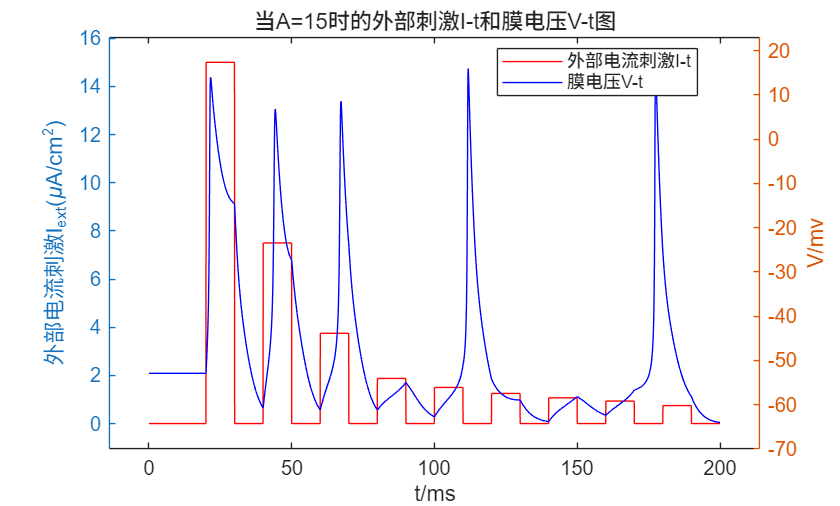
\includegraphics[width=\maxwidth{56.196688409433015em}]{figure_0.png}
\end{center}


\label{TMP_04e9}
\matlabheadingtwo{脉冲刺激2-使用PPT中的参数和方程}

\begin{matlabcode}
% I_ext = @(u) 0+(20<=u & u<= 30).*A...
%     +(40<=u & u<= 50).*A/2 ...
%     +(60<=u & u<= 70).*A/4 ...
%     +(80<=u & u<= 90).*A/8 ...
%     +(100<=u & u<= 110).*A/16 ...
%     +(120<=u & u<= 130).*A/32 ...
A=5;
%脉冲刺激向量
Center=(25:20:185)';%脉冲中心位置,取转置是因为要列向量
% Scale=0.7.^(0:1:8)';%脉冲高度;
Scale=linspace(1,0,9)';
Amplitude=A*Scale;
D1=[Center,Amplitude];%用给pulstran函数,第一列脉冲中心,第二列脉冲高度
PulWidth=10;%脉冲刺激宽度为10ms
PulShap=@(t) rectpuls(t,PulWidth);%脉冲刺激函数
I_ext=@(u) pulstran(u,D1,PulShap);

%脉冲刺激向量

Task1I2V_DC(C,E,g,Alpha,Beta, ...
    'fs',fs, ...
    'T',T, ...
    'A',A, ...
    'I_ext',I_ext);
\end{matlabcode}
\begin{matlaboutput}
此时使用的参数为:
 C: 1.0000 
g的结构体:
    Na: 40
     K: 35
     L: 0.300000000000000

E的结构体:
    Na: 55
     K: -77
     L: -65

Alpha函数的结构体:
    n: @(u)0.02*(u-25)/(1-exp(-(u-25)/9))
    m: @(u)0.182*(u+35)/(1-exp(-(u+35)/9))
    h: @(u)0.25*exp(-(u+90)/12)

Beta函数的结构体:
    n: @(u)-0.002*(u-25)/(1-exp((u-25)/9))
    m: @(u)-0.124*(u+35)/(1-exp((u+35)/9))
    h: @(u)0.25*exp((u+62)/6)/exp((u+90)/12)

外部刺激电流:
    @(u)pulstran(u,D1,PulShap)

当A=5时的外部电流刺激I-t和膜电压V-t图 
\end{matlaboutput}
\begin{center}
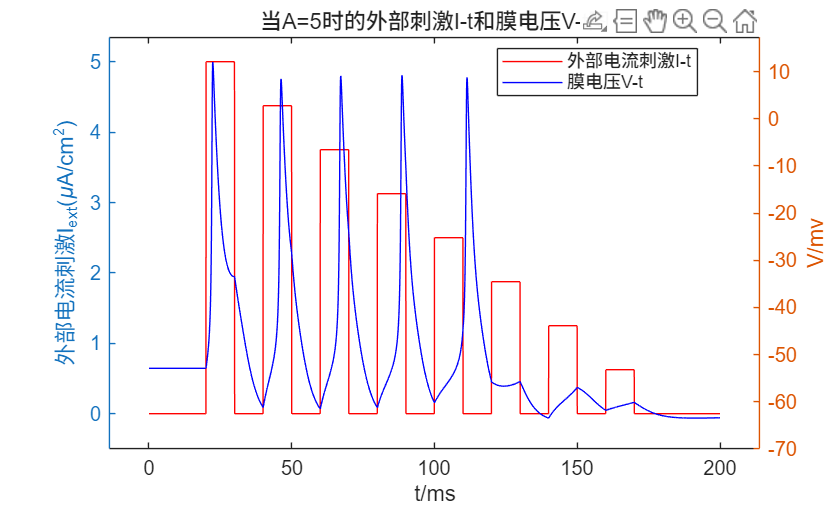
\includegraphics[width=\maxwidth{56.196688409433015em}]{figure_1.png}
\end{center}


\vspace{1em}
\begin{par}
\begin{flushleft}
由此可发现,在刺激电流大于某一阈值时,无论刺激电流大小都会得到相同的膜电压动作电位变化
\end{flushleft}
\end{par}

\begin{par}
\begin{flushleft}
而我们通过一个等比数列递减的外部电流刺激近似得出,大概在第七次时就不能得到膜电压了
\end{flushleft}
\end{par}

\begin{par}
\begin{flushleft}
此时的电流大小为大概在 2.5\textasciitilde{}1.875 mu A/cm\textasciicircum{}2 之间
\end{flushleft}
\end{par}

\begin{matlabcode}
Amplitude(5:6)
\end{matlabcode}
\begin{matlaboutput}
ans = 2x1

2.500000000000000    
1.875000000000000    

\end{matlaboutput}


\vspace{1em}

\label{TMP_8e0c}
\vspace{1em}

\label{TMP_74f9}
\matlabheadingtwo{直流刺激-使用PPT中的参数和方程}

\begin{matlabcode}
% A=5;
% %脉冲刺激向量
% Center=(25:20:185)';%脉冲中心位置,取转置是因为要列向量
% % Scale=0.7.^(0:1:8)';%脉冲高度;
% Scale=linspace(1,0,9)';
% Amplitude=A*Scale;
% D1=[Center,Amplitude];%用给pulstran函数,第一列脉冲中心,第二列脉冲高度
% PulWidth=10;%脉冲刺激宽度为10ms
% PulShap=@(t) rectpuls(t,PulWidth);%脉冲刺激函数
% I_ext=@(u) pulstran(u,D1,PulShap);
for A=2:0.5:5

% A=3;
I_ext = @(u) 0+(20<=u & u<= 150).*A;

%脉冲刺激向量

Task1I2V_DC(C,E,g,Alpha,Beta, ...
    'fs',fs, ...
    'T',T, ...
    'A',A, ...
    'I_ext',I_ext,...
    'Ifdebug',0);

end
\end{matlabcode}
\begin{matlaboutput}
当A=2时的外部电流刺激I-t和膜电压V-t图 
\end{matlaboutput}
\begin{center}
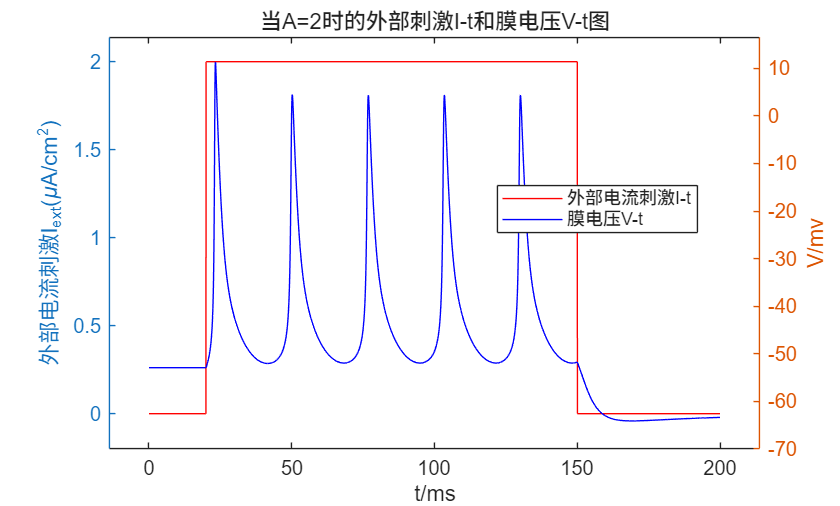
\includegraphics[width=\maxwidth{56.196688409433015em}]{figure_2.png}
\end{center}
\begin{matlaboutput}
当A=2.5时的外部电流刺激I-t和膜电压V-t图 
\end{matlaboutput}
\begin{center}
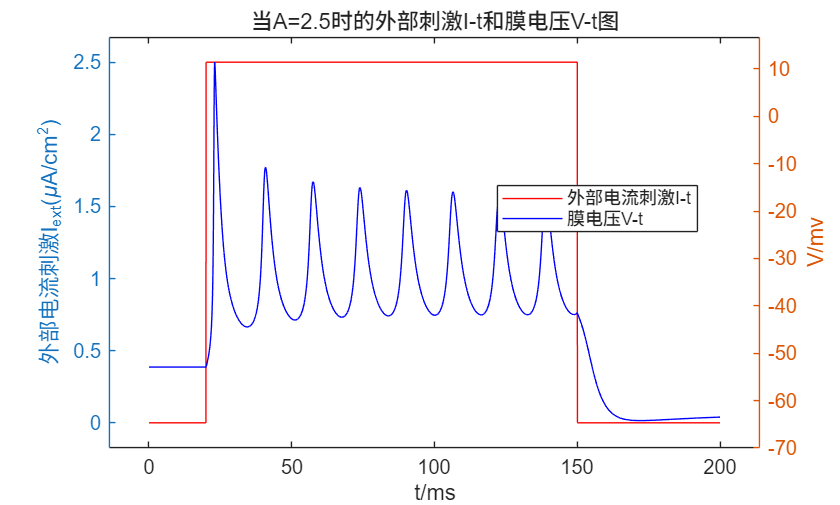
\includegraphics[width=\maxwidth{56.196688409433015em}]{figure_3.png}
\end{center}
\begin{matlaboutput}
当A=3时的外部电流刺激I-t和膜电压V-t图 
\end{matlaboutput}
\begin{center}
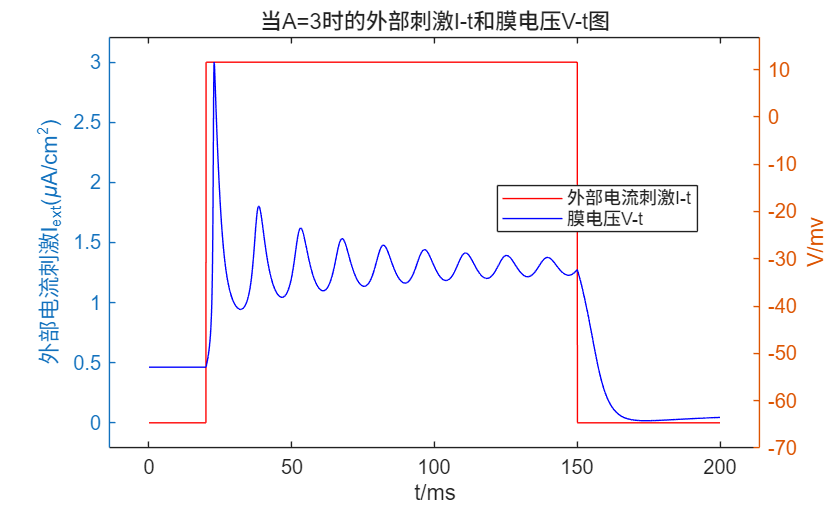
\includegraphics[width=\maxwidth{56.196688409433015em}]{figure_4.png}
\end{center}
\begin{matlaboutput}
当A=3.5时的外部电流刺激I-t和膜电压V-t图 
\end{matlaboutput}
\begin{center}
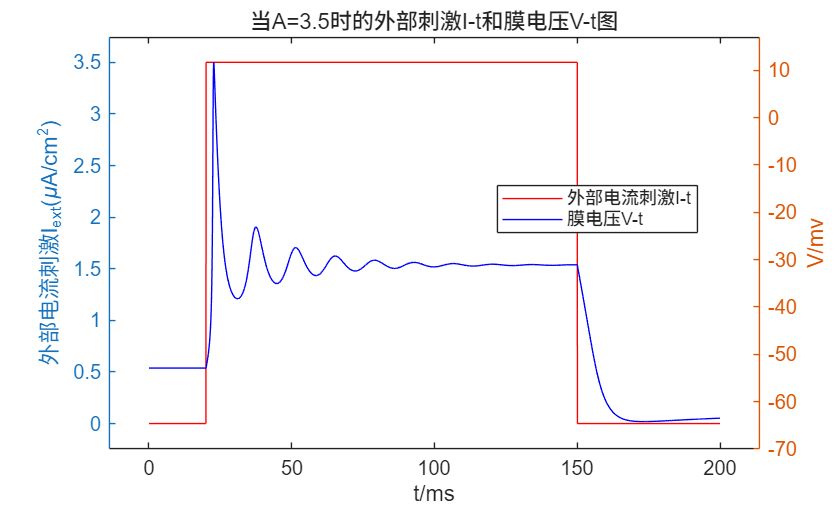
\includegraphics[width=\maxwidth{56.196688409433015em}]{figure_5.png}
\end{center}
\begin{matlaboutput}
当A=4时的外部电流刺激I-t和膜电压V-t图 
\end{matlaboutput}
\begin{center}
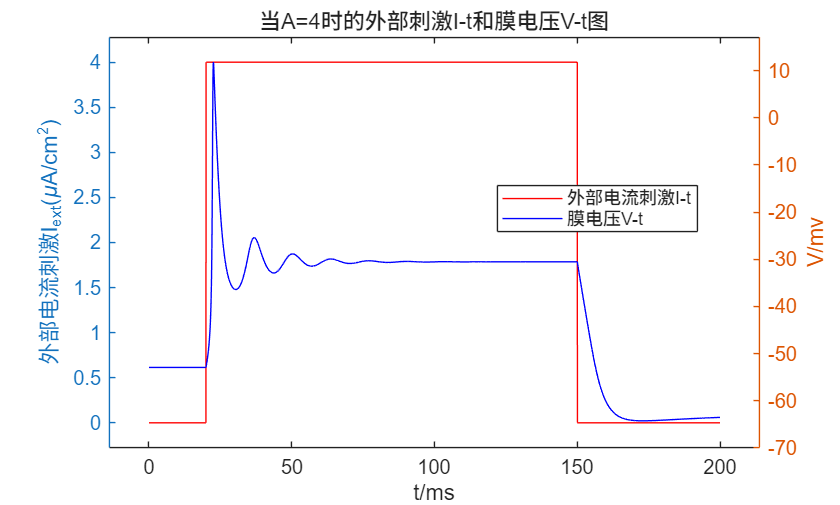
\includegraphics[width=\maxwidth{56.196688409433015em}]{figure_6.png}
\end{center}
\begin{matlaboutput}
当A=4.5时的外部电流刺激I-t和膜电压V-t图 
\end{matlaboutput}
\begin{center}
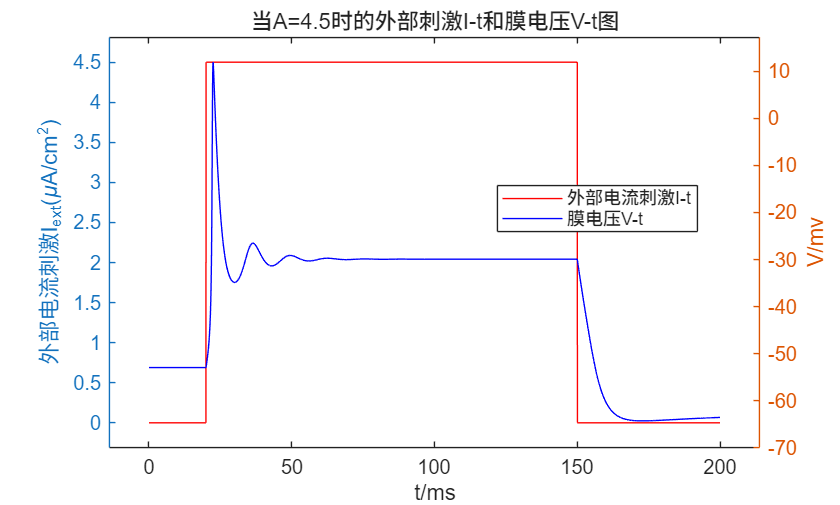
\includegraphics[width=\maxwidth{56.196688409433015em}]{figure_7.png}
\end{center}
\begin{matlaboutput}
当A=5时的外部电流刺激I-t和膜电压V-t图 
\end{matlaboutput}
\begin{center}
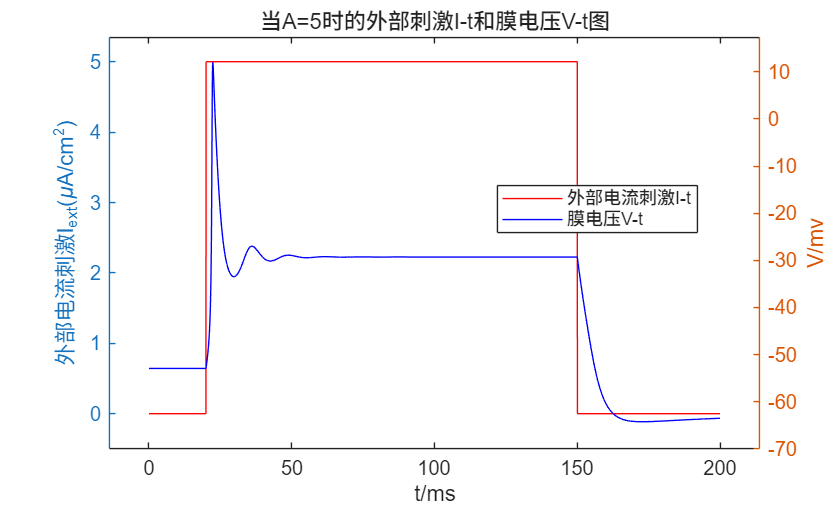
\includegraphics[width=\maxwidth{56.196688409433015em}]{figure_8.png}
\end{center}
\begin{matlabcode}
fprintf('%.5f',A)
\end{matlabcode}
\begin{matlaboutput}
5.00000
\end{matlaboutput}

\begin{par}
\begin{flushleft}
我们发现使用PPT中的参数和alpha,beta函数无法在直流时产生多个动作电位
\end{flushleft}
\end{par}

\begin{par}
\begin{flushleft}
注,应该是以A=3为界限,A\textless{}3时能产生多个动作电位,但是一旦A\textgreater{}3,此时产生的动作电位会趋近于一个
\end{flushleft}
\end{par}

\begin{par}
\begin{flushleft}
这是因为PPT中所使用的模型参数有问题导致的,我们在下面使用另一组参数,只改动常数和alpha beta函数
\end{flushleft}
\end{par}

\begin{par}
\begin{flushleft}
可以立刻得到直流时的多个动作电位
\end{flushleft}
\end{par}


\label{TMP_1e46}
\vspace{1em}

\label{TMP_8e2f}
\matlabheadingtwo{脉冲刺激-使用文献中的参数和方程}


\vspace{1em}
\begin{par}
\begin{flushleft}
《Energy and information in Hodgkin-Huxley neurons》A. Moujahid, A. d’Anjou, and F. J. Torrealdea
\end{flushleft}
\end{par}

\label{TMP_6c4e}
\begin{par}
\begin{flushleft}
中给出的参数是
\end{flushleft}
\end{par}

\begin{par}
\begin{flushleft}
电容:$C=1\mu {\textrm{F/cm}}^2$
\end{flushleft}
\end{par}

\begin{matlabcode}
clc;clear
C=1;
\end{matlabcode}

\begin{par}
\begin{flushleft}
各离子的能斯特电位和对应的电导:
\end{flushleft}
\end{par}

\begin{par}
$$\begin{array}{lrr}
\hline
x & E_x \;\textrm{[mV]} & g_x {\;\textrm{[mS}\;\textrm{/}\;\textrm{cm}}^2 \textrm{]}\\
\hline
\textrm{Na} & 115 & 120\\
\textrm{K} & -12 & 36\\
\textrm{L} & 10.6 & 0.3\\
\hline
\end{array}$$
\end{par}

\begin{matlabcode}
% E.Na=55;E.K=-77;E.L=-65;
% g.Na=40;g.K=35;g.L=0.3;

E.Na=115;E.K=-12;E.L=10.6;
g.Na=120;g.K=36;g.L=0.3;
\end{matlabcode}

\begin{par}
\begin{flushleft}
对应的 alpha和beta函数:
\end{flushleft}
\end{par}

\begin{par}
$$\begin{array}{lcc}
\hline
x & \alpha_x (u/\;\textrm{mV}){\;\textrm{[ms}}^{-1} \textrm{]} & \beta_x (u/\cdot \;\textrm{mV}){\;\textrm{[ms}}^{-1} \textrm{]}\\
\hline
n & (0.1-0.01u)/[\exp (1-0.1u)-1] & 0.125\exp (-u/80)\\
m & (2.5-0.1u)/[\exp (2.5-0.1u)-1] & 4\exp (-u/18)\\
h & 0.07\exp (-u/20) & 1/[\exp (3-0.1u)+1]\\
\hline
\end{array}$$
\end{par}

\begin{matlabcode}
% Alpha.n=@(u) 0.02*(u-25)/(1-exp(-(u-25)/9));
% Alpha.m=@(u) 0.182*(u+35)/(1-exp(-(u+35)/9));
% Alpha.h=@(u) 0.25*exp(-(u+90)/12);
% Beta.n=@(u) -0.002*(u-25)/(1-exp((u-25)/9));
% Beta.m=@(u) -0.124*(u+35)/(1-exp((u+35)/9));
% Beta.h=@(u) 0.25*exp((u+62)/6)/exp((u+90)/12);

Alpha.n=@(u) (0.1 - 0.01.*u) ./ (exp(1 - 0.1.*u) - 1);
Alpha.m=@(u) (2.5 - 0.1.*u) ./ (exp(2.5 - 0.1.*u) - 1);
Alpha.h=@(u) 0.07 .* exp(-u./20);
Beta.n=@(u) 0.125 .* exp(-u./80);
Beta.m=@(u) 4 .* exp(-u./18);
Beta.h=@(u) 1 ./ (exp(3 - 0.1.*u) + 1);
A=3;%刺激电流强度
%脉冲刺激向量
Center=(25:20:185)';%脉冲中心位置,取转置是因为要列向量
% Scale=0.7.^(0:1:8)';%脉冲高度;
Scale=linspace(1,0,9)';
Amplitude=A*Scale;
D1=[Center,Amplitude];%用给pulstran函数,第一列脉冲中心,第二列脉冲高度
PulWidth=10;%脉冲刺激宽度为10ms
PulShap=@(t) rectpuls(t,PulWidth);%脉冲刺激函数
I_ext=@(u) pulstran(u,D1,PulShap);
%脉冲刺激向量

fs= 4000;%采样频率
T=200;%总时长(ms)
% A=15;%刺激电流强度

Task1I2V_DC(C,E,g,Alpha,Beta, ...
    'fs',fs, ...
    'T',T, ...
    'A',A, ...
    'I_ext',I_ext);
\end{matlabcode}
\begin{matlaboutput}
此时使用的参数为:
 C: 1.0000 
g的结构体:
    Na: 120
     K: 36
     L: 0.300000000000000

E的结构体:
    Na: 115
     K: -12
     L: 10.600000000000000

Alpha函数的结构体:
    n: @(u)(0.1-0.01.*u)./(exp(1-0.1.*u)-1)
    m: @(u)(2.5-0.1.*u)./(exp(2.5-0.1.*u)-1)
    h: @(u)0.07.*exp(-u./20)

Beta函数的结构体:
    n: @(u)0.125.*exp(-u./80)
    m: @(u)4.*exp(-u./18)
    h: @(u)1./(exp(3-0.1.*u)+1)

外部刺激电流:
    @(u)pulstran(u,D1,PulShap)

当A=3时的外部电流刺激I-t和膜电压V-t图 
\end{matlaboutput}
\begin{center}
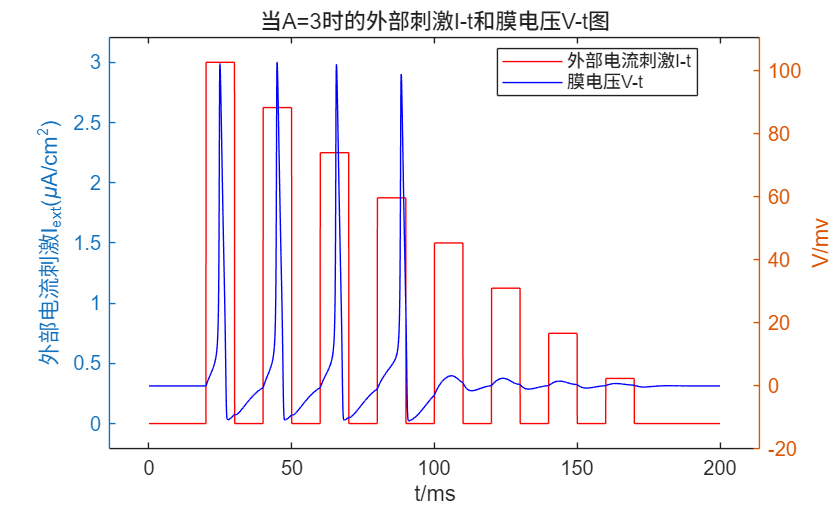
\includegraphics[width=\maxwidth{56.196688409433015em}]{figure_9.png}
\end{center}


\vspace{1em}


\vspace{1em}
\label{TMP_2320}
\matlabheadingtwo{直流刺激-使用文献中的参数和方程}

\begin{par}
\begin{flushleft}
《Energy and information in Hodgkin-Huxley neurons》A. Moujahid, A. d’Anjou, and F. J. Torrealdea
\end{flushleft}
\end{par}

\label{TMP_6c4e}
\begin{par}
\begin{flushleft}
中给出的参数是
\end{flushleft}
\end{par}

\begin{par}
\begin{flushleft}
电容:$C=1\mu {\textrm{F/cm}}^2$
\end{flushleft}
\end{par}

\begin{matlabcode}
clc;clear
C=1;
\end{matlabcode}

\begin{par}
\begin{flushleft}
各离子的能斯特电位和对应的电导:
\end{flushleft}
\end{par}

\begin{par}
$$\begin{array}{lrr}
\hline
x & E_x \;\textrm{[mV]} & g_x {\;\textrm{[mS}\;\textrm{/}\;\textrm{cm}}^2 \textrm{]}\\
\hline
\textrm{Na} & 115 & 120\\
\textrm{K} & -12 & 36\\
\textrm{L} & 10.6 & 0.3\\
\hline
\end{array}$$
\end{par}

\begin{matlabcode}
E.Na=115;E.K=-12;E.L=10.6;
g.Na=120;g.K=36;g.L=0.3;
\end{matlabcode}

\begin{par}
\begin{flushleft}
对应的 alpha和beta函数:
\end{flushleft}
\end{par}

\begin{par}
$$\begin{array}{lcc}
\hline
x & \alpha_x (u/\;\textrm{mV}){\;\textrm{[ms}}^{-1} \textrm{]} & \beta_x (u/\cdot \;\textrm{mV}){\;\textrm{[ms}}^{-1} \textrm{]}\\
\hline
n & (0.1-0.01u)/[\exp (1-0.1u)-1] & 0.125\exp (-u/80)\\
m & (2.5-0.1u)/[\exp (2.5-0.1u)-1] & 4\exp (-u/18)\\
h & 0.07\exp (-u/20) & 1/[\exp (3-0.1u)+1]\\
\hline
\end{array}$$
\end{par}

\begin{matlabcode}
Alpha.n=@(u) (0.1 - 0.01.*u) ./ (exp(1 - 0.1.*u) - 1);
Alpha.m=@(u) (2.5 - 0.1.*u) ./ (exp(2.5 - 0.1.*u) - 1);
Alpha.h=@(u) 0.07 .* exp(-u./20);
Beta.n=@(u) 0.125 .* exp(-u./80);
Beta.m=@(u) 4 .* exp(-u./18);
Beta.h=@(u) 1 ./ (exp(3 - 0.1.*u) + 1);

% for A=[1,5,6,6.5,7,10,15]
for A=[0.001 0.01 0.1 0.5]
% A=5;%刺激电流强度

fs= 4000;%采样频率
T=200;%总时长(ms)
I_ext = @(u) 0+(20<=u & u<= 150).*A;%脉冲刺激向量
[V,m,h,n]=Task1I2V_DC(C,E,g,Alpha,Beta, ...
    'fs',fs, ...
    'T',T, ...
    'A',A, ...
    'I_ext',I_ext,...
    'Ifdebug',0);
end
\end{matlabcode}
\begin{matlaboutput}
直流_当A=0.001时的外部电流刺激I-t和膜电压V-t图 
\end{matlaboutput}
\begin{center}
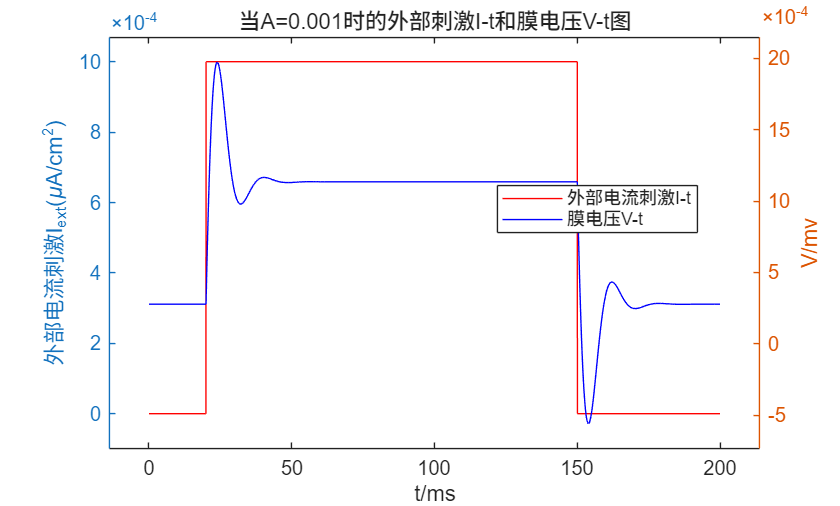
\includegraphics[width=\maxwidth{56.196688409433015em}]{figure_10.png}
\end{center}
\begin{matlaboutput}
直流_当A=0.01时的外部电流刺激I-t和膜电压V-t图 
\end{matlaboutput}
\begin{center}
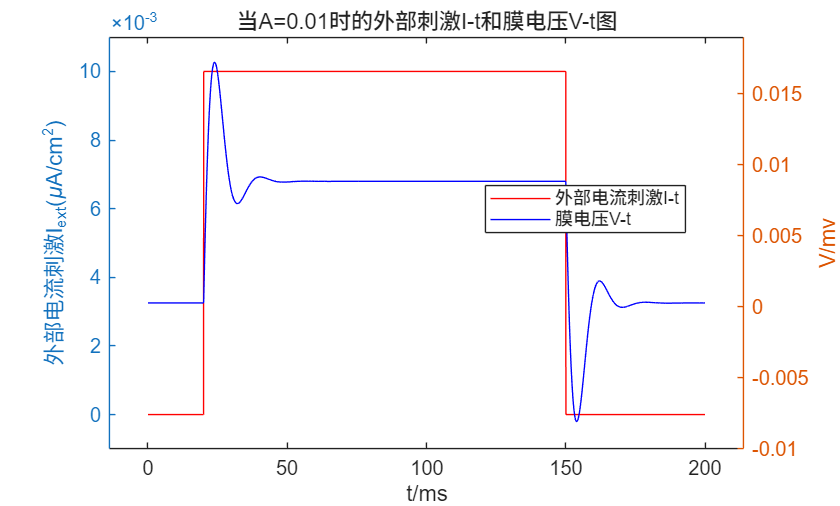
\includegraphics[width=\maxwidth{56.196688409433015em}]{figure_11.png}
\end{center}
\begin{matlaboutput}
直流_当A=0.1时的外部电流刺激I-t和膜电压V-t图 
\end{matlaboutput}
\begin{center}
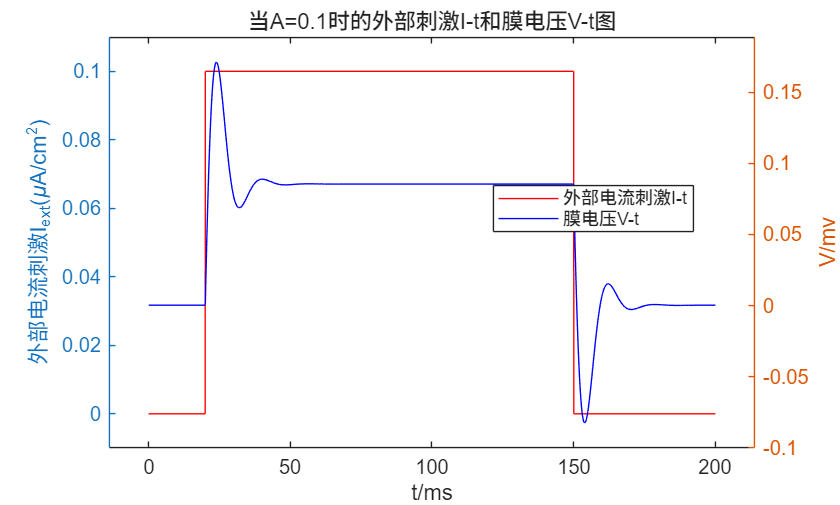
\includegraphics[width=\maxwidth{56.196688409433015em}]{figure_12.png}
\end{center}
\begin{matlaboutput}
直流_当A=0.5时的外部电流刺激I-t和膜电压V-t图 
\end{matlaboutput}
\begin{center}
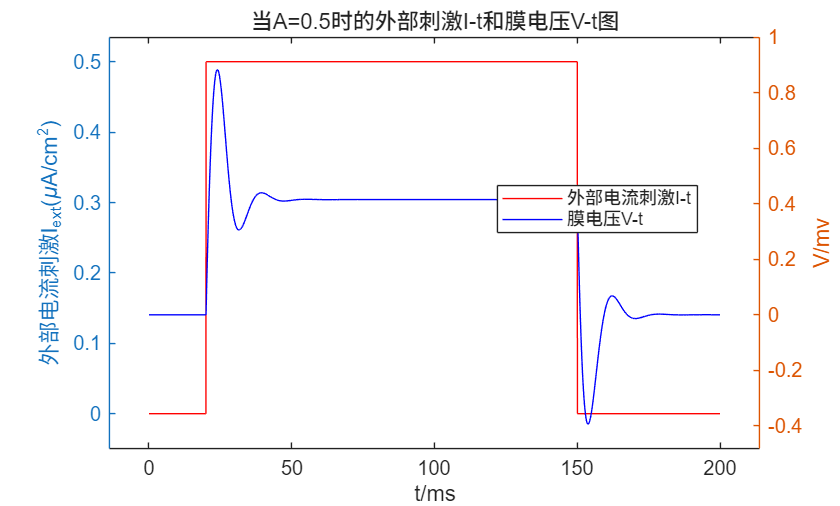
\includegraphics[width=\maxwidth{56.196688409433015em}]{figure_13.png}
\end{center}



\vspace{1em}
\label{TMP_75c0}
\matlabheading{Task2任务 2:计算直流刺激强度和神经元发放频率之间的关系}


\vspace{1em}

\vspace{1em}
\begin{par}
\begin{flushleft}
  试计算直流刺激强度和神经元发放频率之间的关系   (提示: 神经元发放时间的确定)
\end{flushleft}
\end{par}


\vspace{1em}
\begin{par}
\begin{flushleft}
《Energy and information in Hodgkin-Huxley neurons》A. Moujahid, A. d’Anjou, and F. J. Torrealdea
\end{flushleft}
\end{par}

\label{TMP_6c4e}
\begin{par}
\begin{flushleft}
中给出的参数是
\end{flushleft}
\end{par}

\begin{par}
\begin{flushleft}
电容:$C=1\mu {\textrm{F/cm}}^2$
\end{flushleft}
\end{par}

\begin{matlabcode}
clc;clear
tic
C=1;
\end{matlabcode}

\begin{par}
\begin{flushleft}
各离子的能斯特电位和对应的电导:
\end{flushleft}
\end{par}

\begin{par}
$$\begin{array}{lrr}
\hline
x & E_x \;\textrm{[mV]} & g_x {\;\textrm{[mS}\;\textrm{/}\;\textrm{cm}}^2 \textrm{]}\\
\hline
\textrm{Na} & 115 & 120\\
\textrm{K} & -12 & 36\\
\textrm{L} & 10.6 & 0.3\\
\hline
\end{array}$$
\end{par}

\begin{matlabcode}
E.Na=115;E.K=-12;E.L=10.6;
g.Na=120;g.K=36;g.L=0.3;
\end{matlabcode}

\begin{par}
\begin{flushleft}
对应的 alpha和beta函数:
\end{flushleft}
\end{par}

\begin{par}
$$\begin{array}{lcc}
\hline
x & \alpha_x (u/\;\textrm{mV}){\;\textrm{[ms}}^{-1} \textrm{]} & \beta_x (u/\cdot \;\textrm{mV}){\;\textrm{[ms}}^{-1} \textrm{]}\\
\hline
n & (0.1-0.01u)/[\exp (1-0.1u)-1] & 0.125\exp (-u/80)\\
m & (2.5-0.1u)/[\exp (2.5-0.1u)-1] & 4\exp (-u/18)\\
h & 0.07\exp (-u/20) & 1/[\exp (3-0.1u)+1]\\
\hline
\end{array}$$
\end{par}

\begin{matlabcode}
Alpha.n=@(u) (0.1 - 0.01.*u) ./ (exp(1 - 0.1.*u) - 1);
Alpha.m=@(u) (2.5 - 0.1.*u) ./ (exp(2.5 - 0.1.*u) - 1);
Alpha.h=@(u) 0.07 .* exp(-u./20);
Beta.n=@(u) 0.125 .* exp(-u./80);
Beta.m=@(u) 4 .* exp(-u./18);
Beta.h=@(u) 1 ./ (exp(3 - 0.1.*u) + 1);


%%计算静息电位时的初值(在大规模运算时为了提高性能而这样设计)
    fV=@(V,m,h,n,t) 1/C*(-g.L*(V-E.L)-g.Na*m^3*h*(V-E.Na)-g.K*n^4*(V-E.K)+I_ext(t));
    fm=@(V,m) Alpha.m(V)*(1-m)-Beta.m(V)*m;
    fh=@(V,h) Alpha.h(V)*(1-h)-Beta.h(V)*h;
    fn=@(V,n) Alpha.n(V)*(1-n)-Beta.n(V)*n;
    % 为了求解微分方程,我们还必须获得初始值,在静息时,I_ext肯定是0,V,m,h,n的导数也是零
    % 由此可以解方程数值求得初始值,同时也是静息值
    % 使用线性方程解出静息时的电位,各离子浓度比,此时I_ext肯定是0,所以得重新命名一个函数fVT来解方程
    
    syms V0 m0 h0 n0
    fVT=@(V,m,h,n) 1/C*(-g.L*(V-E.L)-g.Na*m^3*h*(V-E.Na)-g.K*n^4*(V-E.K)+0);
    eqt=[fVT(V0,m0,h0,n0),fm(V0,m0)==0,fh(V0,h0)==0,fn(V0,n0)==0];
    VPASol=vpasolve(eqt,[V0 m0 h0 n0]);


% fs= 6000;%采样频率
T = 1000; %总时长(ms)
fs = 13 * T; %采样频率随时间增长而增加,这样可以有效避免解爆炸
t_vec = 0:1 / fs * 1000:T; % 创建时间向量
I_template = (0.1 * T <= t_vec & t_vec <= 0.9 * T); % 预生成电流模板

DelA = 0.1;
Amax = 50;
Avec = 0:DelA:Amax;
N_A = length(Avec);
fPkz = zeros(1, N_A);

toc
\end{matlabcode}
\begin{matlaboutput}
历时 0.065064 秒。
\end{matlaboutput}
\begin{matlabcode}

Count = 1;

% parfor i = 1:N_A %刺激电流强度

%     A = Avec(i);
%     I_ext_vec = A * I_template; %脉冲刺激向量

%     [V, m, h, n] = Task2I2V_fast(C, E, g, Alpha, Beta, VPASol, ...
%         'fs', fs, ...
%         'T', T, ...
%         'A', A, ...
%         'I_ext', I_ext_vec ...
%     );
%     Threold = max(V) * 2/3;
%     % findpeaks(V.*(V>=Threold));
%     [pks, locs] = findpeaks(V .* (V >= Threold));
%     NPkz = length(pks);
%     fPkz(i) = NPkz / (0.8 * T * 1e-3);
%     % disp(fPkz)
% end

fPkz = parfor_Task2I2V_fast(N_A,Avec,I_template, C, E, g, Alpha, Beta, VPASol, fs, T);
\end{matlabcode}
\begin{matlaboutput}
15 / 501 
10 / 501 
30 / 501 
25 / 501 
5 / 501 
20 / 501 
14 / 501 
24 / 501 
4 / 501 
9 / 501 
29 / 501 
19 / 501 
13 / 501 
28 / 501 
23 / 501 
3 / 501 
8 / 501 
18 / 501 
2 / 501 
12 / 501 
7 / 501 
27 / 501 
22 / 501 
17 / 501 
1 / 501 
16 / 501 
11 / 501 
6 / 501 
26 / 501 
21 / 501 
264 / 501 
69 / 501 
225 / 501 
147 / 501 
108 / 501 
186 / 501 
263 / 501 
68 / 501 
224 / 501 
146 / 501 
107 / 501 
185 / 501 
262 / 501 
223 / 501 
145 / 501 
106 / 501 
184 / 501 
67 / 501 
261 / 501 
222 / 501 
144 / 501 
105 / 501 
183 / 501 
66 / 501 
260 / 501 
221 / 501 
143 / 501 
104 / 501 
182 / 501 
65 / 501 
259 / 501 
220 / 501 
142 / 501 
103 / 501 
181 / 501 
64 / 501 
258 / 501 
180 / 501 
141 / 501 
102 / 501 
63 / 501 
219 / 501 
257 / 501 
140 / 501 
101 / 501 
179 / 501 
62 / 501 
218 / 501 
256 / 501 
100 / 501 
178 / 501 
61 / 501 
217 / 501 
139 / 501 
255 / 501 
216 / 501 
138 / 501 
177 / 501 
60 / 501 
99 / 501 
254 / 501 
137 / 501 
176 / 501 
59 / 501 
215 / 501 
98 / 501 
253 / 501 
175 / 501 
58 / 501 
214 / 501 
136 / 501 
97 / 501 
252 / 501 
213 / 501 
57 / 501 
135 / 501 
96 / 501 
174 / 501 
251 / 501 
212 / 501 
173 / 501 
56 / 501 
134 / 501 
95 / 501 
250 / 501 
94 / 501 
172 / 501 
55 / 501 
211 / 501 
133 / 501 
249 / 501 
210 / 501 
171 / 501 
54 / 501 
132 / 501 
93 / 501 
248 / 501 
53 / 501 
209 / 501 
131 / 501 
92 / 501 
170 / 501 
247 / 501 
91 / 501 
169 / 501 
52 / 501 
208 / 501 
130 / 501 
246 / 501 
90 / 501 
168 / 501 
51 / 501 
207 / 501 
129 / 501 
245 / 501 
89 / 501 
167 / 501 
50 / 501 
206 / 501 
128 / 501 
244 / 501 
166 / 501 
88 / 501 
49 / 501 
205 / 501 
127 / 501 
243 / 501 
165 / 501 
204 / 501 
87 / 501 
48 / 501 
126 / 501 
86 / 501 
242 / 501 
164 / 501 
203 / 501 
47 / 501 
125 / 501 
85 / 501 
241 / 501 
163 / 501 
202 / 501 
46 / 501 
124 / 501 
84 / 501 
240 / 501 
162 / 501 
201 / 501 
123 / 501 
45 / 501 
83 / 501 
239 / 501 
161 / 501 
200 / 501 
122 / 501 
44 / 501 
82 / 501 
238 / 501 
160 / 501 
43 / 501 
199 / 501 
121 / 501 
81 / 501 
237 / 501 
159 / 501 
42 / 501 
198 / 501 
120 / 501 
158 / 501 
80 / 501 
236 / 501 
41 / 501 
197 / 501 
119 / 501 
79 / 501 
157 / 501 
235 / 501 
40 / 501 
196 / 501 
118 / 501 
156 / 501 
39 / 501 
117 / 501 
78 / 501 
234 / 501 
195 / 501 
77 / 501 
155 / 501 
116 / 501 
233 / 501 
38 / 501 
194 / 501 
154 / 501 
76 / 501 
37 / 501 
193 / 501 
115 / 501 
232 / 501 
75 / 501 
153 / 501 
36 / 501 
114 / 501 
192 / 501 
231 / 501 
74 / 501 
152 / 501 
35 / 501 
113 / 501 
230 / 501 
191 / 501 
73 / 501 
151 / 501 
34 / 501 
190 / 501 
112 / 501 
229 / 501 
72 / 501 
189 / 501 
111 / 501 
228 / 501 
150 / 501 
33 / 501 
71 / 501 
188 / 501 
110 / 501 
227 / 501 
149 / 501 
32 / 501 
187 / 501 
70 / 501 
226 / 501 
31 / 501 
109 / 501 
148 / 501 
324 / 501 
364 / 501 
304 / 501 
344 / 501 
284 / 501 
384 / 501 
363 / 501 
283 / 501 
323 / 501 
383 / 501 
303 / 501 
343 / 501 
282 / 501 
322 / 501 
382 / 501 
362 / 501 
302 / 501 
342 / 501 
361 / 501 
281 / 501 
321 / 501 
381 / 501 
301 / 501 
341 / 501 
280 / 501 
320 / 501 
380 / 501 
360 / 501 
300 / 501 
340 / 501 
359 / 501 
279 / 501 
299 / 501 
319 / 501 
379 / 501 
339 / 501 
278 / 501 
358 / 501 
298 / 501 
338 / 501 
318 / 501 
378 / 501 
277 / 501 
357 / 501 
337 / 501 
317 / 501 
377 / 501 
297 / 501 
276 / 501 
356 / 501 
316 / 501 
376 / 501 
296 / 501 
336 / 501 
275 / 501 
295 / 501 
335 / 501 
315 / 501 
375 / 501 
355 / 501 
274 / 501 
294 / 501 
314 / 501 
374 / 501 
354 / 501 
334 / 501 
273 / 501 
313 / 501 
353 / 501 
293 / 501 
333 / 501 
373 / 501 
272 / 501 
312 / 501 
352 / 501 
292 / 501 
332 / 501 
372 / 501 
271 / 501 
311 / 501 
351 / 501 
291 / 501 
331 / 501 
371 / 501 
270 / 501 
310 / 501 
350 / 501 
290 / 501 
330 / 501 
370 / 501 
269 / 501 
309 / 501 
349 / 501 
289 / 501 
329 / 501 
369 / 501 
268 / 501 
308 / 501 
288 / 501 
348 / 501 
328 / 501 
368 / 501 
267 / 501 
287 / 501 
307 / 501 
327 / 501 
347 / 501 
367 / 501 
266 / 501 
286 / 501 
306 / 501 
326 / 501 
346 / 501 
366 / 501 
265 / 501 
305 / 501 
285 / 501 
325 / 501 
345 / 501 
365 / 501 
414 / 501 
404 / 501 
394 / 501 
434 / 501 
424 / 501 
444 / 501 
413 / 501 
403 / 501 
393 / 501 
423 / 501 
433 / 501 
443 / 501 
412 / 501 
402 / 501 
392 / 501 
422 / 501 
432 / 501 
442 / 501 
411 / 501 
401 / 501 
391 / 501 
431 / 501 
421 / 501 
441 / 501 
400 / 501 
390 / 501 
410 / 501 
430 / 501 
420 / 501 
440 / 501 
389 / 501 
429 / 501 
399 / 501 
409 / 501 
419 / 501 
439 / 501 
408 / 501 
428 / 501 
388 / 501 
398 / 501 
418 / 501 
438 / 501 
407 / 501 
387 / 501 
427 / 501 
397 / 501 
417 / 501 
437 / 501 
406 / 501 
386 / 501 
426 / 501 
396 / 501 
416 / 501 
436 / 501 
405 / 501 
425 / 501 
385 / 501 
395 / 501 
415 / 501 
435 / 501 
454 / 501 
464 / 501 
449 / 501 
459 / 501 
469 / 501 
474 / 501 
453 / 501 
463 / 501 
458 / 501 
448 / 501 
468 / 501 
473 / 501 
452 / 501 
462 / 501 
447 / 501 
457 / 501 
467 / 501 
472 / 501 
451 / 501 
461 / 501 
456 / 501 
446 / 501 
466 / 501 
471 / 501 
450 / 501 
460 / 501 
445 / 501 
455 / 501 
465 / 501 
470 / 501 
486 / 501 
490 / 501 
482 / 501 
478 / 501 
494 / 501 
498 / 501 
485 / 501 
481 / 501 
477 / 501 
489 / 501 
493 / 501 
497 / 501 
484 / 501 
480 / 501 
476 / 501 
488 / 501 
492 / 501 
496 / 501 
483 / 501 
479 / 501 
487 / 501 
475 / 501 
491 / 501 
495 / 501 
499 / 501 
500 / 501 
501 / 501 

完成。
\end{matlaboutput}
\begin{matlabcode}

figure;
plot(Avec, fPkz)
xlabel('I_{ext} (\muA/cm^2)'), ylabel('f/Hz')
title('直流刺激强度和神经元发放频率之间的关系 I_{ext}-t')
\end{matlabcode}
\begin{center}
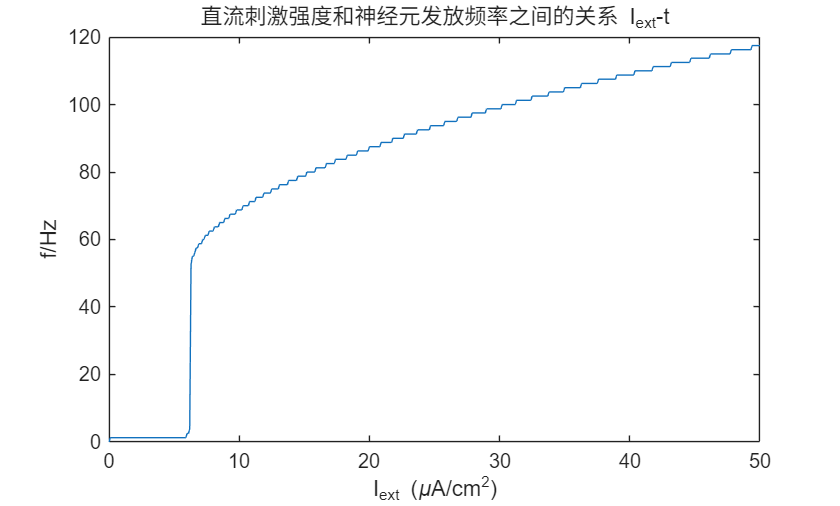
\includegraphics[width=\maxwidth{56.196688409433015em}]{figure_14.png}
\end{center}
\begin{matlabcode}
toc
\end{matlabcode}
\begin{matlaboutput}
历时 72.317596 秒。
\end{matlaboutput}
\begin{matlabcode}

function fPkz = parfor_Task2I2V_fast(N_A,Avec,I_template, C, E, g, Alpha, Beta, VPASol, fs, T)

    %  启动并行池,没有则自动开
    p = gcp('nocreate'); if isempty(p), parpool; end

    %  预分配结果
    fPkz = zeros(1, N_A);

    % 建立数据通道 并 回调(从 worker 发消息到客户端打印进度)
    dq = parallel.pool.DataQueue;
    done = 0;
    afterEach(dq, @onUpdate);

    % 并行循环,do , 报告 完成1次
    parfor i = 1:N_A
        fprintf('%d / %d \n',i,N_A);
        A = Avec(i);
        I_ext_vec = A * I_template; %脉冲刺激向量

        [V, m, h, n] = Task2I2V_fast(C, E, g, Alpha, Beta, VPASol, ...
            'fs', fs, ...
            'T', T, ...
            'A', A, ...
            'I_ext', I_ext_vec ...
        );
        Threold = max(V) * 2/3;
        % findpeaks(V.*(V>=Threold));
        [pks, locs] = findpeaks(V .* (V >= Threold));
        NPkz = length(pks);
        fPkz(i) = NPkz / (0.8 * T * 1e-3);
        % disp(fPkz)
        send(dq, 1); % 告诉客户端又完成了 1 次
    end

    % 换行收尾
    fprintf('\n完成。\n');

    % 客户端回调 每收到一次 send(dq,1) 就更新一回
    function onUpdate(~)
        done = done + 1;
        % 单行覆盖输出 已完成/总数
        fprintf('\r已完成:%d/%d (%.1f%%)', done, N_A, 100 * done / N_A);
    end

end

toc
\end{matlabcode}
\begin{matlaboutput}
历时 72.318415 秒。
\end{matlaboutput}

\begin{par}
\begin{flushleft}
可以看到,我们使用了并行的算法之后性能非常好
\end{flushleft}
\end{par}


\begin{par}
\begin{flushleft}
delA取不同值时的用时如下:
\end{flushleft}
\end{par}

\begin{matlabcode}
x=[0.1,0.3,0.5,0.8,1];
y=[72.318,23.533,14.489,9.13,7.58];
plot(x,y,'-o')
xlabel('delA(\muA/cm^{2})')
ylabel('消耗时间T/s')
title('计算间隔delA-消耗时间T')
\end{matlabcode}
\begin{center}
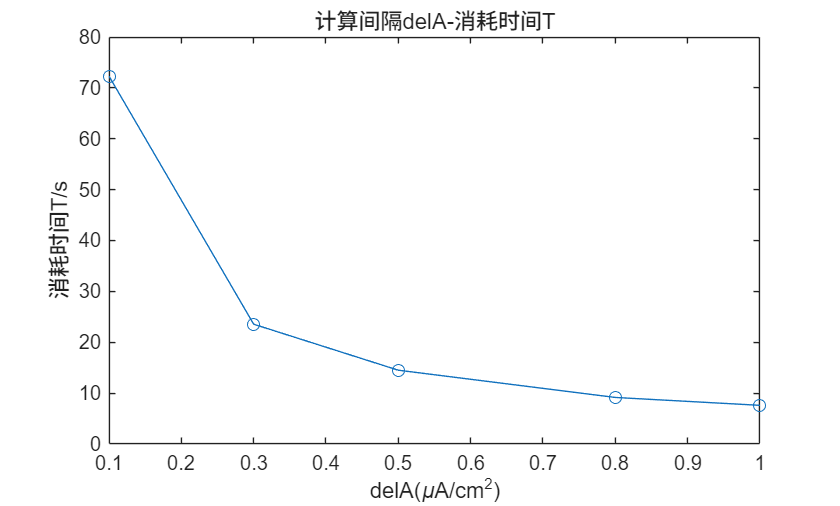
\includegraphics[width=\maxwidth{56.196688409433015em}]{figure_15.png}
\end{center}
\begin{matlabcode}
plot(1./x,y,'-bo')
xlabel('1/delA(cm^{2}/\muA)')
ylabel('消耗时间T/s')
title('计算间隔的倒数1/delA-消耗时间T')
\end{matlabcode}
\begin{center}
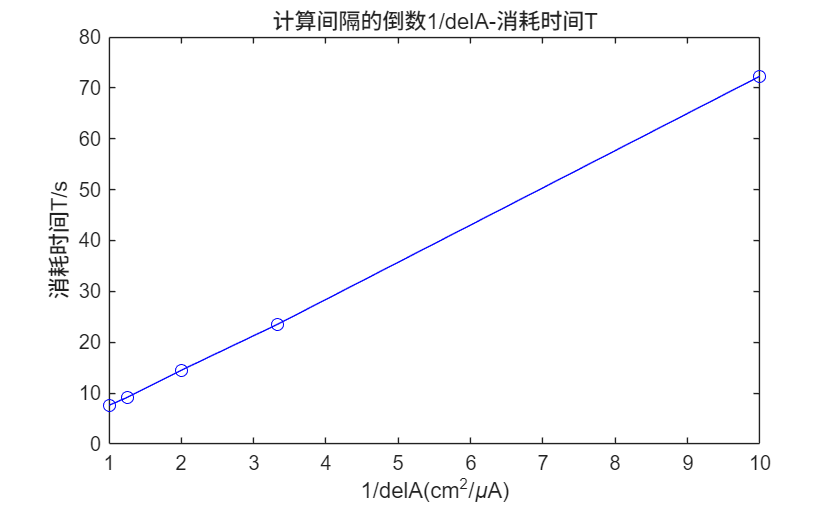
\includegraphics[width=\maxwidth{56.196688409433015em}]{figure_16.png}
\end{center}
\begin{matlabcode}
x_transformed = 1 ./ x;

% p(1) = 斜率, p(2) = 截距
p = polyfit(x_transformed, y, 1);
slope = p(1);
intercept = p(2);

%计算 R^2
y_fit = polyval(p, x_transformed); % 计算拟合后的y值
y_mean = mean(y); % y的平均值
SS_total = sum((y - y_mean).^2); % 总平方和
SS_residual = sum((y - y_fit).^2); % 残差平方和
r_squared = 1 - (SS_residual / SS_total);
fprintf('拟合方程: y = m*(1/x) + c\n');
\end{matlabcode}
\begin{matlaboutput}
拟合方程: y = m*(1/x) + c
\end{matlaboutput}
\begin{matlabcode}
fprintf('斜率 : %.4f\n', slope);
\end{matlabcode}
\begin{matlaboutput}
斜率 : 7.2136
\end{matlaboutput}
\begin{matlabcode}
fprintf('截距: %.4f\n', intercept);
\end{matlabcode}
\begin{matlaboutput}
截距: 0.0421
\end{matlaboutput}
\begin{matlabcode}
fprintf('R^2 : %.6f\n', r_squared);
\end{matlabcode}
\begin{matlaboutput}
R^2 : 0.999849
\end{matlaboutput}

\begin{par}
\begin{flushleft}
\texttt{R\textasciicircum{}2 : 0.999849,可见线性很好,消耗时间是随1/delA线性增加的}
\end{flushleft}
\end{par}



\vspace{1em}
\label{TMP_4eb2}
\matlabheading{Task3任务 3:计算一个动作电势过程中的通过单位面积细胞膜的钠离子总数目}


\vspace{1em}

\vspace{1em}
\begin{par}
\begin{flushleft}
  试计算一个动作电势过程中的通过单位面积细胞膜的钠离子总数目  
\end{flushleft}
\end{par}


\vspace{1em}
\begin{par}
\begin{flushleft}
对一个动作电势过程中的钠电流进行积分, 得到通过钠离子通道的总电量, 除以元电荷电量  
\end{flushleft}
\end{par}


\vspace{1em}
\begin{par}
$$\left\lbrace \begin{array}{l}
C_m \frac{dV}{dt}=-g_L (V-E_L )-{\bar{g} }_{Na} m^3 h(V-E_{Na} )-{\bar{g} }_K n^4 (V-E_K )+I_{app} \\
\frac{dm}{dt}=\alpha_m (V)(1-m)-\beta_m (V)m\\
\frac{dh}{dt}=\alpha_h (V)(1-h)-\beta_h (V)h\\
\frac{dn}{dt}=\alpha_n (V)(1-n)-\beta_n (V)n
\end{array}\right.$$
\end{par}

\begin{par}
\begin{flushleft}
《Energy and information in Hodgkin-Huxley neurons》A. Moujahid, A. d’Anjou, and F. J. Torrealdea
\end{flushleft}
\end{par}

\label{TMP_6c4e}
\begin{par}
\begin{flushleft}
中给出的参数是
\end{flushleft}
\end{par}

\begin{par}
\begin{flushleft}
电容:$C=1\mu {\textrm{F/cm}}^2$
\end{flushleft}
\end{par}

\begin{matlabcode}
clc;clear
C=1;
\end{matlabcode}

\begin{par}
\begin{flushleft}
各离子的能斯特电位和对应的电导:
\end{flushleft}
\end{par}

\begin{par}
$$\begin{array}{lrr}
\hline
x & E_x \;\textrm{[mV]} & g_x {\;\textrm{[mS}\;\textrm{/}\;\textrm{cm}}^2 \textrm{]}\\
\hline
\textrm{Na} & 115 & 120\\
\textrm{K} & -12 & 36\\
\textrm{L} & 10.6 & 0.3\\
\hline
\end{array}$$
\end{par}

\begin{matlabcode}
E.Na=115;E.K=-12;E.L=10.6;
g.Na=120;g.K=36;g.L=0.3;
\end{matlabcode}

\begin{par}
\begin{flushleft}
对应的 alpha和beta函数:
\end{flushleft}
\end{par}

\begin{par}
$$\begin{array}{lcc}
\hline
x & \alpha_x (u/\;\textrm{mV}){\;\textrm{[ms}}^{-1} \textrm{]} & \beta_x (u/\cdot \;\textrm{mV}){\;\textrm{[ms}}^{-1} \textrm{]}\\
\hline
n & (0.1-0.01u)/[\exp (1-0.1u)-1] & 0.125\exp (-u/80)\\
m & (2.5-0.1u)/[\exp (2.5-0.1u)-1] & 4\exp (-u/18)\\
h & 0.07\exp (-u/20) & 1/[\exp (3-0.1u)+1]\\
\hline
\end{array}$$
\end{par}

\begin{matlabcode}
Alpha.n=@(u) (0.1 - 0.01.*u) ./ (exp(1 - 0.1.*u) - 1);
Alpha.m=@(u) (2.5 - 0.1.*u) ./ (exp(2.5 - 0.1.*u) - 1);
Alpha.h=@(u) 0.07 .* exp(-u./20);
Beta.n=@(u) 0.125 .* exp(-u./80);
Beta.m=@(u) 4 .* exp(-u./18);
Beta.h=@(u) 1 ./ (exp(3 - 0.1.*u) + 1);



fs= 4000;%采样频率
T=11;%总时长(ms)
A=15;%刺激电流强度
t=0:T/fs:T;%时间序列向量
Del=t(2)-t(1);%时间间隔
N=length(t);%时间离散化数量

I_ext = @(u) 0+(1<=u & u<= 10).*A;%脉冲刺激向量
[V,m,h,n]=Task3I2V(C,E,g,Alpha,Beta, ...
    'fs',fs, ...
    'T',T, ...
    'A',A, ...
    'I_ext',I_ext);
\end{matlabcode}
\begin{matlaboutput}
此时使用的参数为:
 C: 1.0000 
g的结构体:
    Na: 120
     K: 36
     L: 0.300000000000000

E的结构体:
    Na: 115
     K: -12
     L: 10.600000000000000

Alpha函数的结构体:
    n: @(u)(0.1-0.01.*u)./(exp(1-0.1.*u)-1)
    m: @(u)(2.5-0.1.*u)./(exp(2.5-0.1.*u)-1)
    h: @(u)0.07.*exp(-u./20)

Beta函数的结构体:
    n: @(u)0.125.*exp(-u./80)
    m: @(u)4.*exp(-u./18)
    h: @(u)1./(exp(3-0.1.*u)+1)

外部刺激电流:
    @(u)0+(1<=u&u<=10).*A


下图是外部电流刺激的时域图
\end{matlaboutput}
\begin{center}
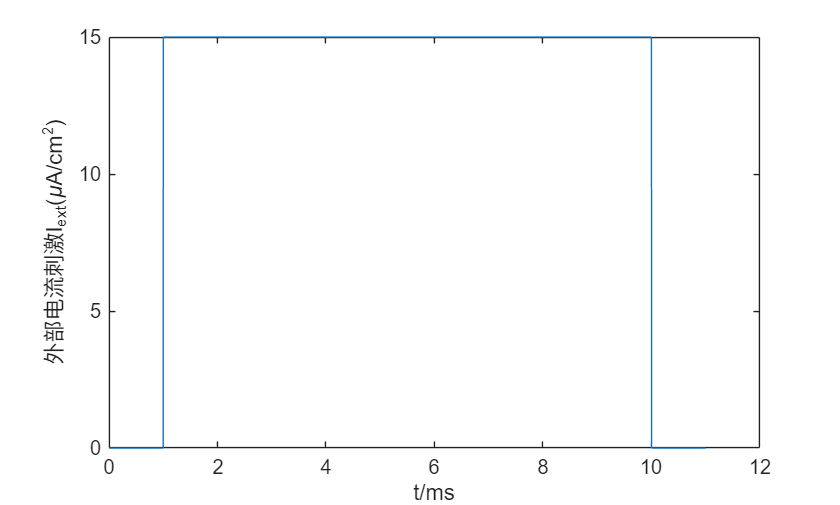
\includegraphics[width=\maxwidth{56.196688409433015em}]{figure_17.png}
\end{center}
\begin{matlaboutput}
下图是膜电压与时间的关系: 
\end{matlaboutput}
\begin{center}
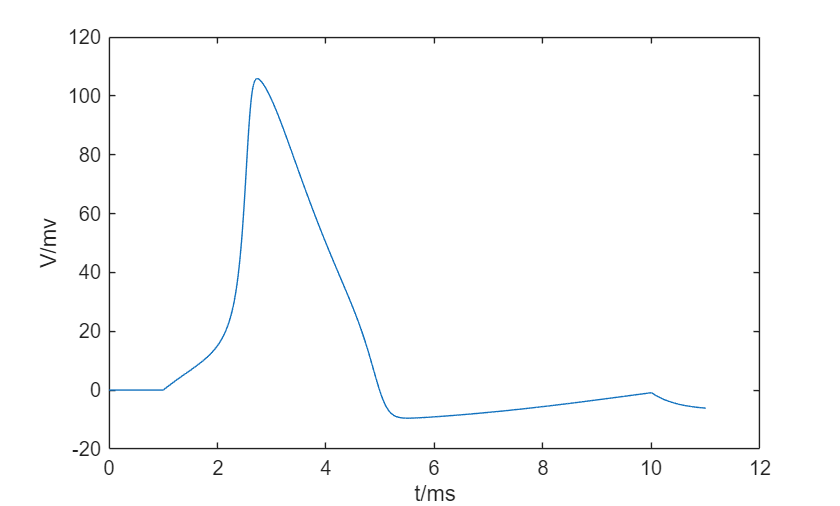
\includegraphics[width=\maxwidth{56.196688409433015em}]{figure_18.png}
\end{center}

\begin{par}
$$C_m \frac{dV}{dt}=-g_L (V-E_L )-{\bar{g} }_{Na} m^3 h(V-E_{Na} )-{\bar{g} }_K n^4 (V-E_K )+I_{app}$$
\end{par}

\begin{matlabcode}
I.K=-g.K.*n.^4.*(V-E.K);
I.L=-g.L.*(V-E.L);
I.Na=-g.Na.*m.^3.*h.*(V-E.Na);
figure;
plot(t,I.K,'b',t,I.L,'r',t,I.Na)
hold on
xlabel('t/ms')
ylabel('I(\muA/cm^2)')
legend('I_{K}','I_{L}','I_{Na}')
\end{matlabcode}
\begin{center}
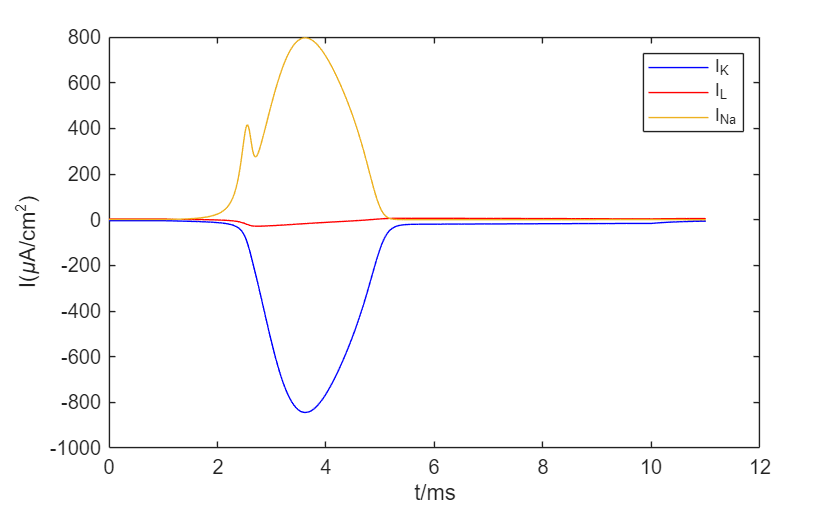
\includegraphics[width=\maxwidth{56.196688409433015em}]{figure_19.png}
\end{center}
\begin{matlabcode}

Qint.K=trapz(t,I.K);
Qint.L=trapz(t,I.L);
Qint.Na=trapz(t,I.Na);
fprintf('穿过膜的各离子电荷量(C):\n')
\end{matlabcode}
\begin{matlaboutput}
穿过膜的各离子电荷量(C):
\end{matlaboutput}
\begin{matlabcode}
disp(Qint)
\end{matlabcode}
\begin{matlaboutput}
     K: -1.540989404456195e+03
     L: -6.326641364649794
    Na: 1.406198873216253e+03
\end{matlaboutput}
\begin{matlabcode}
e=1.602176634e-19 %元电荷电量
\end{matlabcode}
\begin{matlaboutput}
e = 
     1.602176634000000e-19

\end{matlaboutput}
\begin{matlabcode}
Nint.K=Qint.K/e;
Nint.L=Qint.L/e;
Nint.Na=Qint.Na/e;
fprintf('穿过膜的各离子个数:\n')
\end{matlabcode}
\begin{matlaboutput}
穿过膜的各离子个数:
\end{matlaboutput}
\begin{matlabcode}
disp(Nint)
\end{matlabcode}
\begin{matlaboutput}
     K: -9.618099351561225e+21
     L: -3.948778948832052e+19
    Na: 8.776803027675741e+21
\end{matlaboutput}

\begin{par}
\begin{flushleft}
可以看出是
\end{flushleft}
\end{par}

\begin{par}
\begin{flushleft}
穿过膜的各离子个数:
\end{flushleft}
\end{par}

\begin{par}
$$\begin{array}{l}
x~~n_x \\
K~~-9.62\times 10^{21} \textrm{个}\\
L~~-3.95\times 10^{19} \textrm{个}\\
Na~~8.78\times 10^{21} \textrm{个}
\end{array}$$
\end{par}



\vspace{1em}
\label{TMP_5233}
\matlabheading{扩展:}

\begin{par}
\begin{flushleft}
如果 V 是膜电位,电路中在给定时刻累积的总电能为
\end{flushleft}
\end{par}

\begin{par}
$$H(t)=\frac{1}{2}CV^2 +H_{Na} +H_K +H_l ,~~(3)$$
\end{par}

\begin{par}
\begin{flushleft}
其中求和的第一项代表电容器中累积的电能,另外三项分别是电池中的能量。电池中累积的电化学能是未知的。在该模型中,它可能是无限的,因为我们没有考虑电池的耗尽。在真实的神经元中,营养物质的摄入防止了离子泵的耗尽。然而,已知电池向电路提供的电能速率是流过电池的电流乘以其电动势。因此,上述能量对时间的全导数将是
\end{flushleft}
\end{par}

\begin{par}
$$\dot{H} (t)=CV\dot{V} +i_{Na} E_{Na} +i_K E_K +i_l E_l .~~(4)$$
\end{par}

\begin{par}
\begin{flushleft}
设 $I$ 代表以某种方式注入膜的总外部电流。根据方程 (1) 中的第一个方程,我们有
\end{flushleft}
\end{par}

\begin{par}
$$C\dot{V} =I-i_{Na} -i_K -i_l ,$$
\end{par}

\begin{par}
\begin{flushleft}
将其代入方程 (4) 可得
\end{flushleft}
\end{par}

\begin{par}
$$\dot{H} =VI-i_{Na} (V-E_{Na} )-i_K (V-E_K )-i_l (V-E_l ).$$
\end{par}

\begin{par}
\begin{flushleft}
如果我们将方程 (2) 代入离子电流,我们得到电路中的能量速率为
\end{flushleft}
\end{par}

\begin{par}
$$\dot{H} =VI-g_{Na} m^3 h(V-E_{Na} )^2 -g_K n^4 (V-E_K )^2 -g_l (V-E_l )^2 ,~~(5)$$
\end{par}


\vspace{1em}
\begin{par}
\begin{flushleft}
这提供了神经元中电化学能量关于其状态变量的全导数。 右手边求和中的第一项表示通过到达神经元的不同连接给予神经元的电功率,而求和中的其他三项表示离子通道每秒消耗的能量。由于发放率取决于总电流 I, 霍奇金赫胥黎神经元的平均代谢消耗作为发放率的函数可以通过简单评估式(5) 在不同外部电流值下 I。以下两节介绍了这些计算的结果。
\end{flushleft}
\end{par}

\label{TMP_8176}
\matlabheadingthree{Task4动作电位生成中的能量消耗速率}

\begin{par}
\begin{flushleft}
能量供应就是 $VI$,(5)的后三项 $-g_{Na} m^3 h(V-E_{Na} )^2 -g_K n^4 (V-E_K )^2 -g_l (V-E_l )^2$ 就是能量的消耗
\end{flushleft}
\end{par}

\begin{matlabcode}

T=100;%总时长(ms)
fs= 12*T;%采样频率
A=6.9;%刺激电流强度
t=0:T/fs:T;%时间序列向量
Del=t(2)-t(1);%时间间隔
N=length(t);%时间离散化数量

I_ext = @(u) 0+(0.1*T<=u & u<= 0.9*T).*A;%脉冲刺激向量
[V,m,h,n]=Task3I2V(C,E,g,Alpha,Beta, ...
    'fs',fs, ...
    'T',T, ...
    'A',A, ...
    'I_ext',I_ext,...
    'IfPic',0,...
    "IfDebug",0);

Espl=V.*I_ext(t);
Ecost=-g.Na.*m.^3.*h.*(V-E.Na).^2-g.K.*n.^4.*(V-E.K).^2-g.L.*(V-E.L).^2;
figure('Name','动作电位生成中的能量的供给和消耗速率')

subplot(3,1,1);

yyaxis left
plot(t,I_ext(t),'r')
hold on
title('(a)外部电流刺激I_{ext}-t+膜电压V-t')
xlabel('t/ms');
ylabel('I_{ext}(\muA/cm^{2})')

yyaxis right
plot(t,V,'b')
xlabel('t/ms')
ylabel('V/mv')

subplot(3,1,2);
plot(t,Espl,'r');
xlabel('t/ms');
ylabel('E(nJ/s)')
title('(c)能量供给')

subplot(3,1,3);
plot(t,Ecost,'B');
xlabel('t/ms');
ylabel('E(nJ/s)')
title('(d)能量消耗')
\end{matlabcode}
\begin{center}
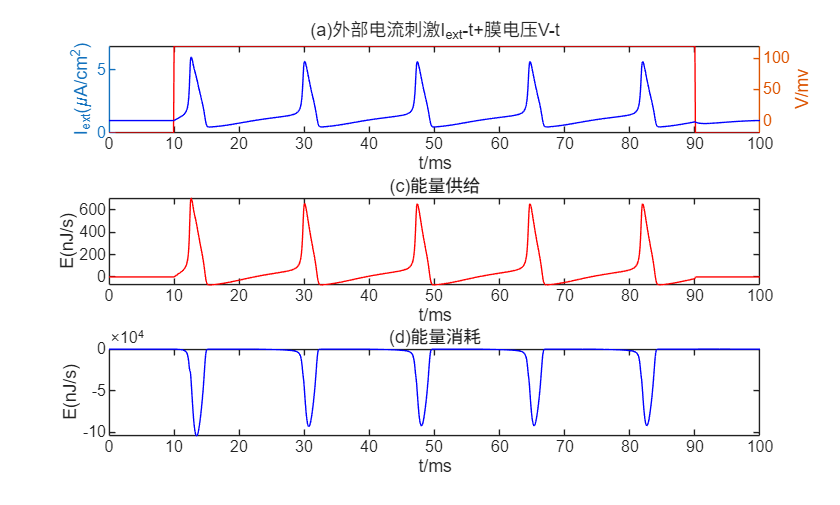
\includegraphics[width=\maxwidth{56.196688409433015em}]{figure_20.png}
\end{center}

\begin{par}
\begin{flushleft}
(a)外部刺激电流时域图,峰值在I = 6.9 $\mu$A (b) 在 I = 6.9 $\mu$A 下生成的动作电位。 (c) 突触连接处每秒的能量供应。 (d) 离子通道处总的每秒的能量耗散。
\end{flushleft}
\end{par}

\begin{par}
\begin{flushleft}
如图(a),外部电流刺激是蜂值为I = 6.9 μA/cm2,持续80ms的方波。在此外部电流值下,神经元以约 58赫兹的频率持续放电。图1(b) 显示了一个生成的动作电位序列。时间以毫秒为单位,膜电位从极化状态下零下几毫伏变化到去极化后的100毫伏。图 1(c) 描绘了随时间变化的电能速率,对应于在方程(5)的右侧的第一项 VI 。它平均为正,峰值达到约600纳焦/秒。它表示对神经元的净能量贡献,其来源取决于电流的来源 I。在实验电极记录的情况下,电极钳制设备将是能量的来源。如果 I 来自突触,这种能量贡献表示在突触连接处每秒供应的能量。在图1(d) 中表示了神经元的总代谢能量消耗。该图描绘了方程(5)的最后三项对能量导数的总贡献。注意它是负的,因为他表示在离子通道处每秒的瞬时总能量消耗。这种电化学能量消耗达到峰值接近100,000nJ/s,并且远大于由 VI 项供应的能量。这种能量速率是否离子泵补充,并通过ATP分 子的水解代谢供应,来维持神经元的活动的。
\end{flushleft}
\end{par}


\vspace{1em}

\begin{par}
\begin{flushleft}
然后我们再来研究一下各个离子的能量消耗功率:
\end{flushleft}
\end{par}

\begin{par}
\begin{flushleft}
    为了方便研究,我们设置成一个动作电位的刺激
\end{flushleft}
\end{par}

\begin{matlabcode}
T=14;%总时长(ms)
fs= 12*T;%采样频率
A=6.9;%刺激电流强度
t=0:T/fs:T;%时间序列向量
Del=t(2)-t(1);%时间间隔
N=length(t);%时间离散化数量

I_ext = @(u) 0+(2<=u & u<= 12).*A;%脉冲刺激向量
[V,m,h,n]=Task3I2V(C,E,g,Alpha,Beta, ...
    'fs',fs, ...
    'T',T, ...
    'A',A, ...
    'I_ext',I_ext,...
    'IfPic',0,...
    "IfDebug",0);


EcostEach.Na=-g.Na.*m.^3.*h.*(V-E.Na).^2;
EcostEach.K=-g.K.*n.^4.*(V-E.K).^2;
EcostEach.L=-g.L.*(V-E.L).^2;

I.K=-g.K.*n.^4.*(V-E.K);
I.L=-g.L.*(V-E.L);
I.Na=-g.Na.*m.^3.*h.*(V-E.Na);



figure('Name','各个离子的能量消耗功率+各离子的电流');
subplot(3,1,1);

yyaxis left
plot(t,I_ext(t),'r')
hold on
title('(a)外部电流刺激I_{ext}-t+膜电压V-t')
xlabel('t/ms');
ylabel('I_{ext}(\muA/cm^{2})')

yyaxis right
plot(t,V,'b')
xlabel('t/ms')
ylabel('V/mv')


subplot(3,1,2)
plot(t,I.K,'b',t,I.L,'r',t,I.Na)
hold on
xlabel('t/ms')
ylabel('I(\muA/cm^2)')
title('(b)各离子的电流')
legend('I_{K}','I_{L}','I_{Na}')
xlim([3 8])

subplot(3,1,3);
plot(t,EcostEach.Na,'g',t,EcostEach.K,'b',t,EcostEach.L,'r');
xlabel('t/ms');
ylabel('E(nJ/s)')
title('(c)各离子的能量消耗')
legend('Na','K','L')
xlim([3 8])
\end{matlabcode}
\begin{center}
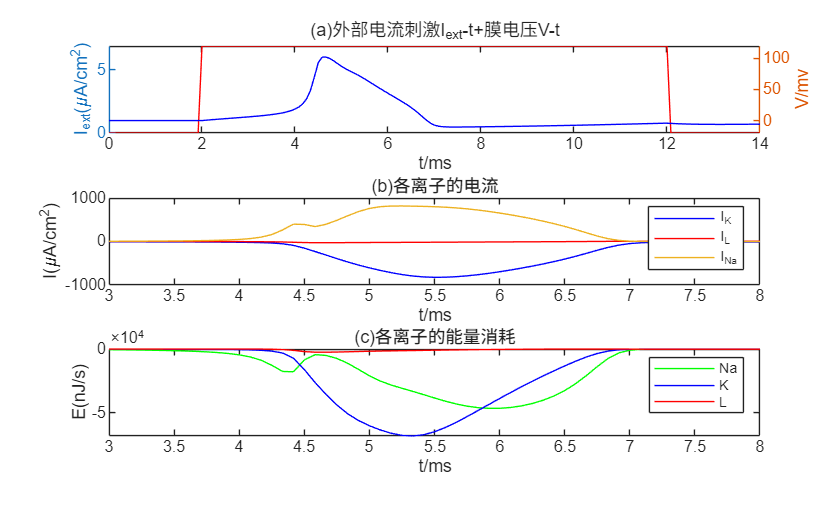
\includegraphics[width=\maxwidth{56.196688409433015em}]{figure_21.png}
\end{center}
\begin{matlabcode}

\end{matlabcode}

\begin{par}
\begin{flushleft}
图 2. (彩色在线) (a)外部刺激电流时域图,峰值在I = 6.9 $\mu$A (b) 在 I = 6.9 $\mu$A 下生成的动作电位。(b) 钠、钾和氯离子在动作电位处的电流。 注意钠电流为负 (c) 对应于各个离子电流的电化学能量消耗,三者均为负。
\end{flushleft}
\end{par}

\begin{par}
\begin{flushleft}
下面是关于'各个离子的能量消耗功率+各离子的电流'图的分析:
\end{flushleft}
\end{par}

\begin{par}
\begin{flushleft}
为了更详细地分析参与动作电位生成的离子电流及 其对能量消耗的贡献,图2(b) 显示了与先前描述的序列中一个特定动作电位对应的钠、钾和氯离子的电流,图 2(c)显示了与每种离子相关的电化学能量消耗。这些电流是响应各自离子电导的变化而产生的,注意钠电流为负值。 钠电流在约 815 μA/cm2处达到峰值,钾电流在约 -823 μA/cm2处达到峰值;泄漏电流则小得多。请注意,由于钠和钾电流都携带正电荷但在细胞膜上向相反方向移动,它们在相互重叠的范围内相互中和,因此净膜电流要小得多。
\end{flushleft}
\end{par}

\begin{par}
\begin{flushleft}
然而,无论离子是否协作建立膜电位,离子的实际运动都会发生并涉及能量消耗。在动作电位期间渗透膜的Na+离子总数与图中钠电流曲线下的面积成正比。
\end{flushleft}
\end{par}

\begin{par}
$$\begin{array}{l}
x~~n_x \\
K~~-9.62\times 10^{21} \textrm{个}\\
L~~-3.95\times 10^{19} \textrm{个}\\
Na~~8.78\times 10^{21} \textrm{个}
\end{array}$$
\end{par}

\begin{par}
\begin{flushleft}
如第一节所述, 这个Na+ 离子总数用于估算离子泵重新建立离子浓度所需的ATP分子数量。图2(c)显示了与每种离子电流相关的电化学能量平衡。三个离子通道对方程(5)中的能量导数有负贡献,所以在图像中是负的。请注意,在我们的方法中,神经元生成一个动作电位的代谢消耗直接是这三个分量的总和。重新建立三种离子Na+、K+和 Cl+ 的浓度需要能量,并且该方法与它们是否在每次泵循环中使用一个ATP分子一起移动无关。
\end{flushleft}
\end{par}



\vspace{1em}
\label{TMP_30ae}
\matlabheadingthree{Task5平均能量消耗作为外部电流的函数}

\begin{par}
\begin{flushleft}
神经元的瞬时能量消耗并不直接令人感兴趣,因为它在动作电位生成的时间跨度内持续变化,单位时间平均值更为有用。
\end{flushleft}
\end{par}

\begin{par}
\begin{flushleft}
为了研究神经元平均代谢消耗与其发放率相关的变化程度,我们在1000ms的长时间内平均了不同外部电流值下的离子电流和离子消耗 I。
\end{flushleft}
\end{par}

\begin{matlabcode}
% 拓展:平均能量消耗作为外部电流的函数
clc; clear

tic
% 《Energy and information in Hodgkin-Huxley neurons》A. Moujahid, A. d'Anjou, and F. J. Torrealdea
% 中给出的参数是

% 电容:
C = 1;

% 各离子的能斯特电位和对应的电导:
E.Na = 115; E.K = -12; E.L = 10.6;
g.Na = 120; g.K = 36; g.L = 0.3;

% 对应的 alpha和beta函数:
Alpha.n = @(u) (0.1 - 0.01 .* u) ./ (exp(1 - 0.1 .* u) - 1);
Alpha.m = @(u) (2.5 - 0.1 .* u) ./ (exp(2.5 - 0.1 .* u) - 1);
Alpha.h = @(u) 0.07 .* exp(-u ./ 20);
Beta.n = @(u) 0.125 .* exp(-u ./ 80);
Beta.m = @(u) 4 .* exp(-u ./ 18);
Beta.h = @(u) 1 ./ (exp(3 - 0.1 .* u) + 1);

%%计算静息电位时的初值(在大规模运算时为了提高性能而这样设计)
fV = @(V, m, h, n, t) 1 / C * (-g.L * (V - E.L) - g.Na * m ^ 3 * h * (V - E.Na) - g.K * n ^ 4 * (V - E.K) + I_ext(t));
fm = @(V, m) Alpha.m(V) * (1 - m) - Beta.m(V) * m;
fh = @(V, h) Alpha.h(V) * (1 - h) - Beta.h(V) * h;
fn = @(V, n) Alpha.n(V) * (1 - n) - Beta.n(V) * n;
% 为了求解微分方程,我们还必须获得初始值,在静息时,I_ext肯定是0,V,m,h,n的导数也是零
% 由此可以解方程数值求得初始值,同时也是静息值
% 使用线性方程解出静息时的电位,各离子浓度比,此时I_ext肯定是0,所以得重新命名一个函数fVT来解方程

syms V0 m0 h0 n0
fVT = @(V, m, h, n) 1 / C * (-g.L * (V - E.L) - g.Na * m ^ 3 * h * (V - E.Na) - g.K * n ^ 4 * (V - E.K) + 0);
eqt = [fVT(V0, m0, h0, n0), fm(V0, m0) == 0, fh(V0, h0) == 0, fn(V0, n0) == 0];
VPASol = vpasolve(eqt, [V0 m0 h0 n0]);

% fs= 6000;%采样频率
T = 1000; %总时长(ms)
fs = 13 * T; %采样频率随时间增长而增加,这样可以有效避免解爆炸
t_vec = 0:T / fs :T; % 创建时间向量
% I_template = (0.1 * T <= t_vec & t_vec <= 0.9 * T); % 预生成电流模板
I_template = (0<= t_vec & t_vec <=  T); % 预生成电流模板
DelA = 0.01;
Amax = 50;
Avec = 0:DelA:Amax;
N_A = length(Avec);
fPkz = zeros(1, N_A);
% EcostEach.Na=zeros(1, N_A);
% EcostEach.K=zeros(1, N_A);
% EcostEach.L=zeros(1, N_A);
% 
% I.K=zeros(1, N_A);
% I.L=zeros(1, N_A);
% I.Na=zeros(1, N_A);
Espl=zeros(1, N_A);%平均能量供应
EcostEach(N_A) = struct('Na', [], 'K', [], 'L', []);%平均能量消耗
I(N_A)         = struct('Na', [], 'K', [], 'L', []);%平均电流
Qint(N_A) = struct('Na', [], 'K', [], 'L', []);
Nint(N_A) = struct('Na', [], 'K', [], 'L', []);
toc
\end{matlabcode}
\begin{matlaboutput}
历时 0.112062 秒。
\end{matlaboutput}
\begin{matlabcode}
Count = 1;

% parfor i = 1:N_A %刺激电流强度

%     A = Avec(i);
%     I_ext_vec = A * I_template; %脉冲刺激向量

%     [V, m, h, n] = Task2I2V_fast(C, E, g, Alpha, Beta, VPASol, ...
%         'fs', fs, ...
%         'T', T, ...
%         'A', A, ...
%         'I_ext', I_ext_vec ...
%     );
%     Threold = max(V) * 2/3;
%     % findpeaks(V.*(V>=Threold));
%     [pks, locs] = findpeaks(V .* (V >= Threold));
%     NPkz = length(pks);
%     fPkz(i) = NPkz / (0.8 * T * 1e-3);
%     % disp(fPkz)
% end

[fPkz, EcostEach, I,Espl,Qint,Nint]  = parfor_TaskProI2V_fast(N_A,Avec,I_template, C, E, g, Alpha, Beta, VPASol, fs, T);
\end{matlabcode}
\begin{matlaboutput}
完成。
\end{matlaboutput}


\begin{matlabcode}
ProE_IfigName="平均能量消耗作为外部电流的函数,DelA="+DelA;
ProE_Ifig=figure('Name',ProE_IfigName);
subplot(3,2,1)
plot(Avec, fPkz)
xlabel('I_{ext} (\muA/cm^2)'), ylabel('f/Hz')
title('(a)直流刺激强度和神经元发放频率之间的关系 I_{ext}-f')

subplot(3,2,2)%每秒各离子平均总能量消耗作为施加电流 I 的函数
plot(Avec, [EcostEach.Na],'r',Avec,[EcostEach.K],'g',Avec,[EcostEach.L],'b')
xlabel('I_{ext} (\muA/cm^2)'), ylabel('meanEcost(nJ/s)')
title('(b)直流刺激强度和各离子平均能量消耗之间的关系 I_{ext}-meanEcost')
legend('Na','K','L','Location','best')

subplot(3,2,3)%在不同外部施加电流 I 值下,长动作电位序列上钠和钾电流的平均值
plot(Avec, [I.Na],'r',Avec,[I.K],'g',Avec,[I.L],'b')
xlabel('I_{ext} (\muA/cm^2)'), ylabel('meanEcost(nJ/s)')
title('(c)直流刺激强度和各离子平均电流之间的关系I_{ext}-meanEcost')
legend('Na','K','L','Location','bestoutside')

subplot(3,2,4)%通过注射部位供应给神经元的每秒平均能量
plot(Avec,  Espl )
xlabel('I_{ext} (\muA/cm^2)'), ylabel('meanEsupply(nJ/s)')
title('(d)直流刺激强度和能量供应之间的关系 I_{ext}-meanEsupply')

EcostAll=[EcostEach.Na]+[EcostEach.K]+[EcostEach.L];

subplot(3,2,5)%每秒各离子平均总能量消耗作为施加电流 I 的函数
plot(Avec, abs(EcostAll))
xlabel('I_{ext} (\muA/cm^2)'), ylabel('meanEcost(nJ/s)')
title('(e)直流刺激强度和总的平均能量消耗之间的关系 I_{ext}-meanEcostAll')
legend('EcostEach,Na+K+L','Location','best')


e=1.602176634e-19; %元电荷电量
subplot(3,2,6)%总能量消耗与钠离子数量三分之一的比率。该比率以电子伏特每ATP表示,并在模型中表示ATP水解的效率,测量为由一分子ATP水解提供的自由能。
plot(Avec, abs(EcostAll./([Nint.Na]./3))./e)%除e是因为单位是(eV/ATP)
xlabel('I_{ext} (\muA/cm^2)'), ylabel('水解效率(eV/ATP)')
title('(f)总能量消耗与钠离子数量三分之一的比率')
% legend('EcostEach,Na+K+L','Location','best')
sgtitle("注:此时的计算精度是:相邻两点的电流间隔是DelA="+DelA)
% xlim([0,30])
saveas(ProE_Ifig,ProE_IfigName+'.fig','fig')
\end{matlabcode}

\begin{par}
\begin{flushleft}
然后我们再将 e d f图放大,以便观察什么时候会发生突变
\end{flushleft}
\end{par}

\begin{matlabcode}
ProE_IfigZoomName=ProE_IfigName+'Zoom'
\end{matlabcode}
\begin{matlaboutput}
ProE_IfigZoomName = "平均能量消耗作为外部电流的函数,DelA=0.01Zoom"
\end{matlaboutput}
\begin{matlabcode}
ProE_IfigZoom=figure('Name',ProE_IfigZoomName);
Lx=1.5;Rx=8;
subplot(3,1,1)%通过注射部位供应给神经元的每秒平均能量
plot(Avec,  Espl )
xlim([Lx Rx])
xlabel('I_{ext} (\muA/cm^2)'), ylabel('meanEsupply(nJ/s)')
title('(d)直流刺激强度和能量供应之间的关系 I_{ext}-meanEsupply')

EcostAll=[EcostEach.Na]+[EcostEach.K]+[EcostEach.L];

subplot(3,1,2)%每秒各离子平均总能量消耗作为施加电流 I 的函数
plot(Avec, abs(EcostAll))
xlim([Lx Rx])
xlabel('I_{ext} (\muA/cm^2)'), ylabel('meanEcost(nJ/s)')
title('(e)直流刺激强度和总的平均能量消耗之间的关系 I_{ext}-meanEcostAll')
legend('EcostEach,Na+K+L','Location','northwest')


e=1.602176634e-19; %元电荷电量
subplot(3,1,3)%总能量消耗与钠离子数量三分之一的比率。该比率以电子伏特每ATP表示,并在模型中表示ATP水解的效率,测量为由一分子ATP水解提供的自由能。
plot(Avec, abs(EcostAll./([Nint.Na]./3))./e)%除e是因为单位是(eV/ATP)
xlim([Lx Rx])
xlabel('I_{ext} (\muA/cm^2)'), ylabel('水解效率(eV/ATP)')
title('(f)总能量消耗与钠离子数量三分之一的比率')
sgtitle("注:此时的计算精度是:相邻两点的电流间隔是DelA="+DelA)
% xlim([0,30])
saveas(ProE_IfigZoom,ProE_IfigZoomName+'.fig','fig')
% 总能量消耗与钠离子数量三分之一的比率。该比率以电子伏特每ATP表示,并在模型中表示ATP水解的效率,测量为由 一分子ATP水解提供的自由能。

toc
\end{matlabcode}
\begin{matlaboutput}
历时 612.137483 秒。
\end{matlaboutput}
\begin{matlabcode}

function [fPkz, EcostEach, I,Espl,Qint,Nint] = parfor_TaskProI2V_fast(N_A,Avec,I_template, C, E, g, Alpha, Beta, VPASol, fs, T)

    %  启动并行池,没有则自动开
    p = gcp('nocreate'); if isempty(p), parpool; end

    %  预分配结果
    fPkz = zeros(1, N_A);

    % 建立数据通道 并 回调(从 worker 发消息到客户端打印进度)
    dq = parallel.pool.DataQueue;
    done = 0;
    afterEach(dq, @onUpdate);

    % 并行循环,do , 报告 完成1次
    parfor i = 1:N_A
        % fprintf('%d / %d \n',i,N_A);
        A = Avec(i);
        I_ext_vec = A * I_template; %脉冲刺激向量

        [V, m, h, n] = Task2I2V_fast(C, E, g, Alpha, Beta, VPASol, ...
            'fs', fs, ...
            'T', T, ...
            'A', A, ...
            'I_ext', I_ext_vec ...
            );
  
   
        % E_Na_series = -g.Na.*m.^3.*h.*(V-E.Na).^2;
        % E_K_series  = -g.K.*n.^4.*(V-E.K).^2;
        % E_L_series  = -g.L.*(V-E.L).^2;

        %各离子平均能量消耗
        EcostEach(i).Na=mean(-g.Na.*m.^3.*h.*(V-E.Na).^2);
        EcostEach(i).K=mean(-g.K.*n.^4.*(V-E.K).^2);
        EcostEach(i).L=mean(-g.L.*(V-E.L).^2);

        Espl(i)=mean(V.*I_ext_vec);%平均能量供应

        %各离子平均电流
        I(i).K=mean(-g.K.*n.^4.*(V-E.K));
        I(i).L=mean(-g.L.*(V-E.L));
        I(i).Na=mean(-g.Na.*m.^3.*h.*(V-E.Na));

        % 有了电流,可以计算交换的电荷量和离子数
        IK=-g.K.*n.^4.*(V-E.K);
        IL=-g.L.*(V-E.L);
        INa=-g.Na.*m.^3.*h.*(V-E.Na);
        %穿过膜的各离子电荷量
         t=0:T/fs:T;%时间序列向量
        QK=trapz(t,IK);
        QL=trapz(t,IL);
        QNa=trapz(t,INa);

        Qint(i).K=QK;
        Qint(i).L=QL;
        Qint(i).Na=QNa;
        % fprintf('穿过膜的各离子电荷量(C):\n')
        % disp(Qint)
        e=1.602176634e-19 %元电荷电量
        %穿过膜的各离子个数
        Nint(i).K=QK/e;
        Nint(i).L=QL/e;
        Nint(i).Na=QNa/e;
        % fprintf('穿过膜的各离子个数:\n')
        % disp(Nint)

        %每次A取值时的频率计算
        Threold = max(V) * 2/3;
        % findpeaks(V.*(V>=Threold));
        [pks, locs] = findpeaks(V .* (V >= Threold));
        NPkz = length(pks);
        fPkz(i) = NPkz / (0.8 * T * 1e-3);

        % disp(fPkz)
        send(dq, 1); % 告诉客户端又完成了 1 次
    end

    % 换行收尾
    fprintf('\n完成。\n');

    % 客户端回调 每收到一次 send(dq,1) 就更新一回
    function onUpdate(~)
        done = done + 1;
        % 单行覆盖输出 已完成/总数
        fprintf('\r已完成:%d/%d (%.1f%%)', done, N_A, 100 * done / N_A);
    end

end

\end{matlabcode}

\begin{par}
\begin{flushleft}
图3(a) 显示了 长序列动作电位的钠和钾电流的平均值。对于外部电流 的值 I 在I = 4 和 6.2 μA/cm2 神经元处于静息状态而不发放。在此区域,钠通道的小电导使该电流保持在非常低的值。钾电流略大,补偿了泄漏和外部电流。
\end{flushleft}
\end{par}

\begin{par}
\begin{flushleft}
对于较大的外部电流值 I ,神经元获得递增发放率的强直发放状态。钠和钾电流的平均值清楚地检测到过渡并随着发放率的增加而增加。
\end{flushleft}
\end{par}

\begin{par}
\begin{flushleft}
在图3(b) 中,显示了单位时间总能量消耗(所有三个通道)作为施加电流 I 函数的平均值。能量消耗的垂直突然增加清楚地揭示了从低电流值 I 下的静息状态无发放到由较大施加电流 值诱导的发放状态的过渡。与尖峰生成相关的更高能量需求清晰可见;
\end{flushleft}
\end{par}

\begin{par}
\begin{flushleft}
例如,在 I = 6.9 μA/cm2,处,这是先前 分析的动作电位序列生成所用的值,平均代谢消耗约为 9000 nJ/s。此消耗必须通过代谢ATP供应来补充。对应于不同电流值 I 的发放频率显示在插图中。
\end{flushleft}
\end{par}

\begin{par}
\begin{flushleft}
图3(c) 显示 了由 V I 项提供给神经元的每秒平均能量。它随电流 I 线性增加,在静息和发放状态下具有不同的斜率。它始终远低于离子通道的耗散。
\end{flushleft}
\end{par}

\begin{par}
\begin{flushleft}
在图3(d) 中,显示了总能量消耗与通过膜的钠离子数三分之一的比值。该比值以电子伏特每ATP表示,并代表ATP水解的效率,测量为在模型中由一个ATP分子水解提供的自由能。如图所示,该比值在整个 I 在I = 6.2 和 10 μA/cm2值范围内是恒定的; 也就是说,它与发放率无关。
\end{flushleft}
\end{par}

\begin{par}
\begin{flushleft}
因此,我们的结果表明,在发放期间,钠钾泵要求每个ATP分子0.39电子伏特,这与文献中估计的一个泵送周期(将两个钾离子移入细胞和三个钠离子移出细胞) 的0.37电子伏特非常一致 [20]。这一结果也与报道的数据一致,即一个ATP分子可以释放0.43电子伏特的自由能 [21],, 
\end{flushleft}
\end{par}

\begin{par}
\begin{flushleft}
这意味着ATP使用效率很高,只有10\%的释放自由能以热能形式损失。另一方面,当神经元处于静息状态时,模型中ATP水解所需的效率为0.51电子伏特,略大于一个ATP 分子可以释放的能量。这一结果指出霍奇金‐赫胥黎模型在神经元静息时低估了钠离子的数量。
\end{flushleft}
\end{par}


\vspace{1em}
\label{TMP_2a0b}
\vspace{1em}


\vspace{1em}
\label{TMP_3078}
\matlabheadingtwo{Task6两个电耦合神经元的能量平衡}


\vspace{1em}

\vspace{1em}
\begin{par}
\begin{flushleft}
间隙连接通道允许两个神经元的细胞内电位直接连接在一起,通常被称为电突触。当两个或多个神经元耦合在一起时,它们很常见,并在细胞事件的同步中发挥重要作用。特别是,它们在传输信息和同步神经元群的信息方面很高效 [22]。尽管对称性是电突触的预期特性, 但文献中也报道了不对称间隙连接。例如,在视网膜中, 有证据表明信号传输从AII无长突细胞到ON锥双极细胞的方向比另一个方向更有效 [18]。这种功能整流可以通过两种细胞类型之间膜输入电阻的相应差异来解释。在本工作中,为了保持信息传输的明确方向,我们研究了完全不对称的单向间隙连接。
\end{flushleft}
\end{par}


\vspace{1em}
\label{TMP_4200}
\matlabheadingthree{单向耦合的定义}


\vspace{1em}
\begin{par}
\begin{flushleft}
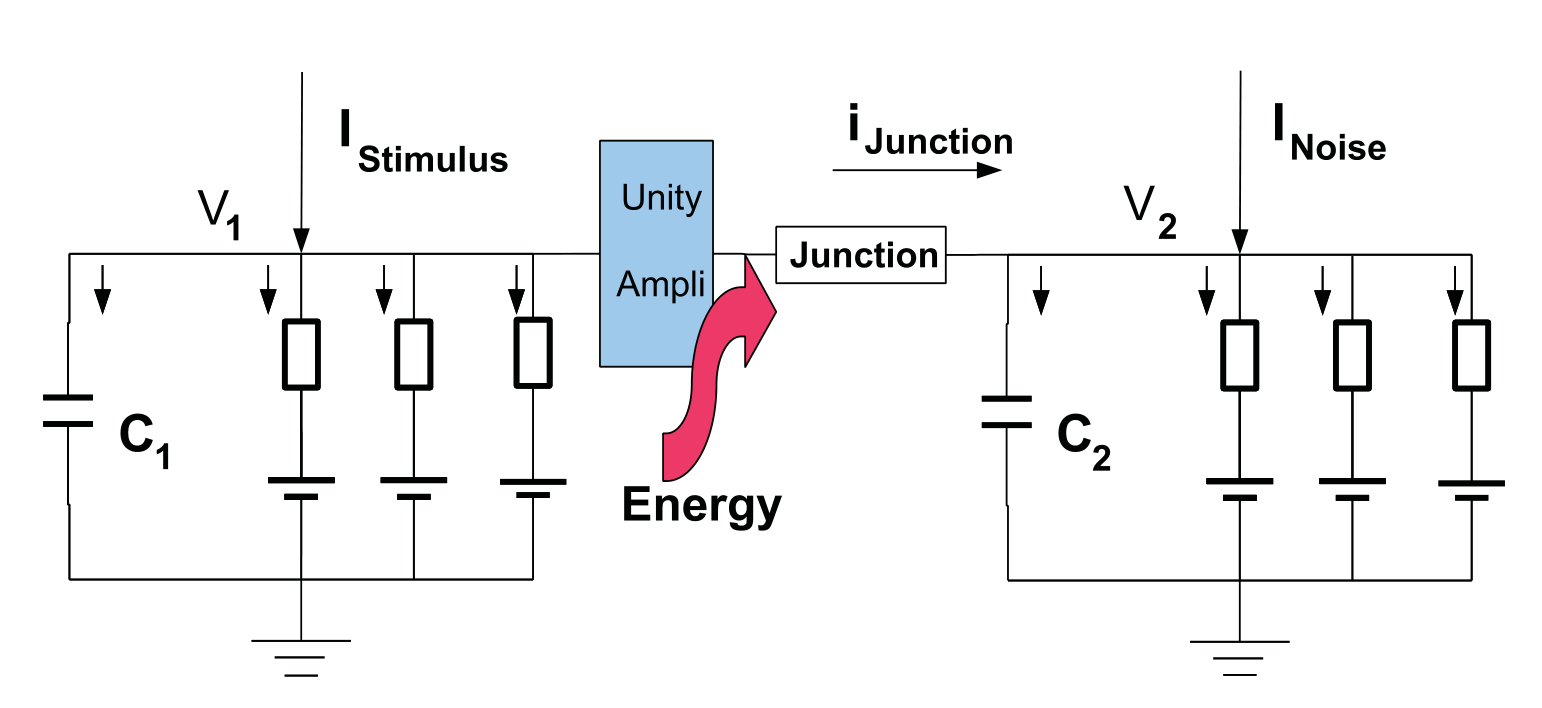
\includegraphics[width=\maxwidth{34.92222779729052em}]{image_3}
\end{flushleft}
\end{par}

\begin{par}
\begin{flushleft}
图4.电单向耦合;霍奇金‑赫胥黎电路。
\end{flushleft}
\end{par}


\vspace{1em}
\begin{par}
\begin{flushleft}
间隙连接通道可以直接连接两个神经元的胞体或在神经突的末端形成接触位点。无论如何,我们认为接触位点不贡献于电路的电容 [22]。两个神经元都遵守方程集(1)并附加一个影响突触后神经元的耦合。
\end{flushleft}
\end{par}

\begin{par}
$$\begin{array}{rcl}
C\dot{V}  & = & -i_{Na} -i_K -i_l +I,\\
\dot{m}  & = & \alpha_m (V)(1-m)-\beta_m (V)m,\\
\dot{n}  & = & \alpha_n (V)(1-n)-\beta_n (V)n,\\
\dot{h}  & = & \alpha_h (V)(1-h)-\beta_h (V)h,
\end{array}~~(1)$$
\end{par}

\begin{par}
\begin{flushleft}
突触前神经元的膜电流密度已被表示为 $I_{\textrm{Stimulus}} (t)$,一个推测由兴奋性外部刺激诱导的电流。它已被建模为均值 $0\,\mu \textrm{A}$ 和方差 $9\,\mu \textrm{A}$ 的高斯噪声。高斯噪声的刺激输入参数均值和方差已通过实验选择,以便它们在突触前神经元的脉冲序列中产生足够的变异性。这个熵的脉冲序列在我们的工作中保持统计不变,并已被用作信息源。
\end{flushleft}
\end{par}


\vspace{1em}
\begin{par}
\begin{flushleft}
突触后神经元,推测是一个中间神经元,暴露于一个总噪声电流 $I_{\textrm{noise}}$,该电流被建模为均值 $0\,\mu \textrm{A}$ 和方差 $1\,\mu \textrm{A}$ 的高斯噪声。这个噪声可以推测为到达突触后神经元的不规则信号的均值,来自我们不特别考虑的其他突触。这个噪声没有引入到突触前神经元,在将其视为刺激电流的一部分方面没有特殊困难。
\end{flushleft}
\end{par}


\vspace{1em}
\begin{par}
\begin{flushleft}
每个神经元的膜电位的两个方程是:
\end{flushleft}
\end{par}

\begin{par}
$$C_1 \dot{V_1 } =I_{\textrm{Stimulus}} (t)-i_{1Na} -i_{1K} -i_{1l} ,~~(6)$$
\end{par}

\begin{par}
$$C_2 \dot{V_2 } =I_{\textrm{Noise}} (t)-i_{2Na} -i_{2K} -i_{2l} +I_{\textrm{Junction}} .$$
\end{par}


\vspace{1em}
\begin{par}
\begin{flushleft}
通过连接的电流是 $I_{\textrm{Junction}} =k(V_1 -V_2 )$,其中参数 $k\;$是间隙连接的电导,或称耦合强度,单位是 ${\textrm{mS/cm}}^2$。电流 $I_{\textrm{Stimulus}} (t)$ 代表刺激突触前神经元的可变电流,该电流携带由神经元传输的信息, 而 $I_{\textrm{Noise}} (t)$ 表示通过其他突触到达突触后神经元的总噪声电流。
\end{flushleft}
\end{par}


\vspace{1em}
\begin{par}
\begin{flushleft}
因此,在单向耦合中,不允许电流从突触前神经元流入或流出。然而,连接电流 $k(V_1 -V_2 )$ 仍然必须通过电连接流入接收神经元。图4展示了一个可能的电路,该电路实现了两个霍奇金‐赫胥黎神经元之间的单向耦合。 连接处的电势差由一个具有单位增益和极高输入阻抗的放大器维持,该放大器使第一个神经元在能量上独立于第二个神经元。突触后神经元在连接处所需的能量由放大器提供。放大器提供电流 $I_{\textrm{Junction}}$ 在电压 $V_1$;也就是说, 功率 $V_1 I_{\textrm{Junction}}$。对应于突触后神经元的电路中的电能, 这是唯一受耦合影响的部分,现在是:
\end{flushleft}
\end{par}

\begin{par}
$$H_2 (t)=\frac{1}{2}C_2 V_2^2 +H_{2Na} +H_{2K} +H_{2l} +H_{\textrm{Amplifier}} ,~~(7)$$
\end{par}

\begin{par}
\begin{flushleft}
这是电容器中累积的电能加上三个电池中的电化学能量加上放大器中可用能量的总和。第二个神经元中的总能量导数由:
\end{flushleft}
\end{par}

\begin{par}
$$\dot{H_2 } =V_2 I_{\textrm{noise}} -g_{2Na} m_2^3 h_2 (V_2 -E_{2Na} )^2 -g_{2K} n_2^4 (V_2 -E_{2K} )^2 -g_{2l} (V_2 -E_{2l} )^2 +kV_2 (V_1 -V_2 )+kV_1 (V_1 -V_2 ).~~(8)$$
\end{par}

\begin{par}
\begin{flushleft}
三个离子通道在这个导数右侧的联合贡献在整篇论文中被用来计算突触后神经元的代谢消耗。最后两项代表突触中的能量平衡,这对应于在突触的突触后部位消耗的能量加上由放大器贡献的能量。注意,突触中这个代谢能量的净消耗不一定是负的,因此突触本身可能是一个主动供应者。无论如何,能量并非来自信号神经元,它提供信息但不提供能量。
\end{flushleft}
\end{par}


\vspace{1em}
\label{TMP_9dd0}
\matlabheadingthree{单向耦合的计算结果}


\vspace{1em}
\begin{matlabcode}
% demo_fig5_fig6_parallel.m — (并行加速)
% 注意需要和 run_HH_coupling_single_k.m放在同一文件夹中
clear; clc;  
% 基本 HH 参数
C = 1;
E.Na = 115; E.K = -12; E.L = 10.6;
g.Na = 120; g.K = 36; g.L = 0.3;
% Alpha/Beta 不再需要,因为它们已内联到函数中

% 仿真选项 (打包到 opt 结构体中)
opt.fs      = 2e4;          % 20 kHz → dt=0.05 ms
opt.T       = 3.0e4;        % 30 s = 30000 ms
opt.T_warm  = 3.0e3;        % 丢弃前 3 s 热启动
opt.mu_pre     = 8.4;       % 调整后的值,原论文这里设置的是0,显然不合理
opt.sigma_pre  = 3.0;
opt.mu_post    = 0.0;
opt.sigma_post = 1.0;
opt.seed    = 20251029;
opt.Ifdebug = 1;            % 调试开关

k_list  = 0:0.01:0.20;  % k 扫描
K = numel(k_list);
fprintf('开始并行计算 %d 个 k 值 (T=%.1f s)...\n', K, opt.T/1000);

% 并行计算
% 使用元胞数组 (cell array) 来收集不同结构体
OUT_cell = cell(1, K); 
parfor ik = 1:K
    % 不再传递 Alpha 和 Beta
    OUT_cell{ik} = run_HH_coupling_single_k(k_list(ik), C,E,g,opt);
end

fprintf('计算完成,正在重组数据...\n');

% --- 数据重组 ---
% 将元胞数组转换为结构体数组,然后再解包
OUT_array = [OUT_cell{:}]; 

OUT.k                 = [OUT_array.k];
OUT.Pchan_pre_mean    = [OUT_array.Pchan_pre_mean];
OUT.Pchan_post_mean   = [OUT_array.Pchan_post_mean];
OUT.Fr_pre            = [OUT_array.Fr_pre];
OUT.Fr_post           = [OUT_array.Fr_post];
OUT.P_amp_mean        = [OUT_array.P_amp_mean];
OUT.P_diss_post_mean  = [OUT_array.P_diss_post_mean];
OUT.P_net_mean        = [OUT_array.P_net_mean];

%% 绘图
% 图 5
figure('Name','图5 — 不同 k 下发送/接收神经元通道平均代谢能耗','Color','w');
plot(OUT.k, OUT.Pchan_pre_mean,  '-o','LineWidth',1.5); hold on;
plot(OUT.k, OUT.Pchan_post_mean, '-s','LineWidth',1.5);
xlabel('突触电导  k  (mS/cm^2)');
ylabel('平均代谢能量消耗(通道总和,pJ/ms·cm^{-2})');
title('图5.(彩色在线)k 变化下发送/接收神经元离子通道的平均代谢能耗(单向耦合)');
legend({'发送神经元(s)','接收神经元(r)'},'Location','northwest','Box','off');
grid on;
axes('Position',[0.60 0.30 0.32 0.32]);
plot(OUT.k, OUT.Fr_pre,  '-o','LineWidth',1.2); hold on;
plot(OUT.k, OUT.Fr_post, '--^','LineWidth',1.2);
xlabel('k'); ylabel('Hz'); title('平均放电频率');
legend({'s','r'},'Location','best','Box','off'); grid on;
% 图 6
figure('Name','图6 — 外介质供能与突触后部耗散(功率)','Color','w');
plot(OUT.k, OUT.P_amp_mean,       '-^','LineWidth',1.5); hold on;
plot(OUT.k, OUT.P_diss_post_mean, '-s','LineWidth',1.5);
xlabel('突触电导  k  (mS/cm^2)');
ylabel('功率(nJ/s·cm^{-2} ≡ pJ/ms·cm^{-2})');
title('图6.(彩色在线)从细胞外介质供能与突触后部位耗散(单向耦合)');
legend({'从外介质供能(放大器项)','突触后部位耗散'},'Location','northwest','Box','off');
grid on;
axes('Position',[0.60 0.30 0.32 0.32]);
plot(OUT.k, OUT.P_net_mean,'-o','LineWidth',1.2);
xlabel('k'); ylabel('pJ/ms·cm^{-2}'); 
title('连接处净能量导数 \langle P_{supply} + P_{dissip} \rangle'); 
grid on;

% figure('Name',' — 不同 k 下发送/接收神经元通道平均代谢能耗','Color','w');
% plot(OUT.k, OUT.Pchan_pre_mean,  '-','LineWidth',1.5); hold on;
% plot(OUT.k, OUT.Pchan_post_mean, '-','LineWidth',1.5);
% xlabel('突触电导  k  (mS/cm^2)');
% ylabel('平均代谢能量消耗(通道总和,pJ/ms·cm^{-2})');
% title('k 变化下发送/接收神经元离子通道的平均代谢能耗(单向耦合)');
% legend({'发送神经元(s)','接收神经元(r)'},'Location','northwest','Box','off');
% grid on;
% axes('Position',[0.60 0.30 0.32 0.32]);
% plot(OUT.k, OUT.Fr_pre,  '-','LineWidth',1.2); hold on;
% plot(OUT.k, OUT.Fr_post, '-','LineWidth',1.2);
% xlabel('k'); ylabel('Hz'); title('平均放电频率');
% legend({'s','r'},'Location','best','Box','off'); grid on;
% % 图 6
% figure('Name',' — 外介质供能与突触后部耗散(功率)','Color','w');
% plot(OUT.k, OUT.P_amp_mean,       '-','LineWidth',1.5); hold on;
% plot(OUT.k, OUT.P_diss_post_mean, '-','LineWidth',1.5);
% xlabel('突触电导  k  (mS/cm^2)');
% ylabel('功率(nJ/s·cm^{-2} ≡ pJ/ms·cm^{-2})');
% title('从细胞外介质供能与突触后部位耗散(单向耦合)');
% legend({'从外介质供能(放大器项)','突触后部位耗散'},'Location','northwest','Box','off');
% grid on;
% axes('Position',[0.60 0.30 0.32 0.32]);
% plot(OUT.k, OUT.P_net_mean,'-','LineWidth',1.2);
% xlabel('k'); ylabel('pJ/ms·cm^{-2}'); 
% title('连接处净能量导数 \langle P_{supply} + P_{dissip} \rangle'); 
% grid on;
\end{matlabcode}

\begin{par}
\begin{flushleft}
平均代谢能量消耗,作为耦合电导的函数 $k$,对于单向耦合的两个神经元,如图5所示。代谢能量消耗是通过方程(7)中所有三个离子项的贡献计算的,对于突触后神经元,以及突触前神经元的等效项。由于脉冲序列是嘈杂的,一些随机特性(如能量消耗速率)的收敛需要长时间的平均。为了执行这个计算,平均值取自一个750秒长的动作电位序列。曲线是针对耦合电导绘制的 $k$, 并且我们在表示中反转了能量导数的实际负号。由于耦合是单向的,连接的电导对突触前神经元没有影响,其平均代谢能量消耗保持恒定在约 $9000\,\textrm{nJ/s}$。突触后神经元起始于 $k=0\,{\textrm{mS/cm}}^2$,消耗约 $500\,\textrm{nJ/s}$,这对应于其静息状态,偶尔被随机兴奋所改变。随着耦合强度的增加,代谢消耗逐渐增加,直到在耦合强度值约为 $k=0.1\,{\textrm{mS/cm}}^2$ 时,达到几乎与突触前神经元相同的消耗水平。 此时,突触后神经元的放电频率已达到突触前神经元的水平。平均放电频率如插图所示。
\end{flushleft}
\end{par}


\vspace{1em}
\begin{par}
\begin{flushleft}
图5.(彩色在线)在不同突触电导 $k$ 值下,发送和接收神经元离子通道的平均代谢能量消耗。突触前神经元的刺激电流 $I_{\textrm{Stimulus}} (t)$,推测由兴奋性外部刺激引起,已建模为均值 $0\,\mu \textrm{A}$、 方差 $9\,\mu \textrm{A}$ 的高斯噪声。突触后神经元,推测是负责传输信息的中间神经元,暴露于总噪声电流 $I_{\textrm{noise}}$,推测通过我们未具体考虑的其他突触到达,建模为均值 $0\,\mu \textrm{A}$、方差 $1\,\mu \textrm{A}$ 的高斯噪声。 插图显示了两个神经元的平均放电频率作为电导 $k$ 的函数。单向耦合。
\end{flushleft}
\end{par}


\vspace{1em}
\begin{par}
\begin{flushleft}
图6. (彩色在线) 从细胞外介质供应的每秒平均能量和在突触后部位向细胞外介质的平均耗散,在不同突触电导 $k$ 值下。 插图中显示了连接处的净能量导数,其为正的;也就是说,从突触有能量的净收入。单向耦合。
\end{flushleft}
\end{par}


\vspace{1em}
\begin{par}
\begin{flushleft}
我们还分析了单向突触连接中的能量平衡。由于神经元之间不能有任何能量流动,突触后神经元只能与细胞外环境交换离子和能量,尽管受突触前神经元控制。 在图6中,突触代谢能量的两个组成部分,即方程(7)的最后两项,已针对耦合电导绘制 $k$。第一项平均总是负的,表示在连接处的能量耗散。第二项总是正的,表示放大器传递给神经元的能量,代表从外部环境进入连接处的能量。因此,突触后神经元在连接处既耗散又吸收能量。图6中的插图显示了两部分的联合贡献。可以看出,对于神经元来说,平衡是正的;也就是说,通过突触位置有一个净的(尽管很小)能量收入,且该输入能量在高于 $k=0.04\,{\textrm{mS/cm}}^2$ 时达到一个尖锐的最大值。如图5所示,以及更清楚地在第III节中对于一组突触后神经元(见图10),在耦合电导的该值处,突触后神经元的代谢能量消耗似乎存在一个拐点。这一事实的相关性我们尚不清楚。
\end{flushleft}
\end{par}


\vspace{1em}

\vspace{1em}
\begin{par}
\begin{flushleft}
  对“Hodgkin-Huxley 神经元中的能量与信息”的评论  
\end{flushleft}
\end{par}

\begin{par}
\begin{flushleft}
Hideo Hasegawa 
\end{flushleft}
\end{par}

\begin{par}
\begin{flushleft}
 日本东京 184-8501 小金井市,东京学艺大学物理系 
\end{flushleft}
\end{par}

\begin{par}
\begin{flushleft}
(日期:2011 年 6 月 30 日)
\end{flushleft}
\end{par}

\begin{par}
\begin{flushleft}
  摘要  
\end{flushleft}
\end{par}

\begin{par}
\begin{flushleft}
在最近的一篇论文 [A. Moujahid, A. d'Anjou, F. J. Torrealdea and F. Torrealdea, Phys. Rev. E 83, 031912 (2011)] 中,作者们使用 Hodgkin-Huxley (HH) 模型(霍奇金-赫胥黎模型)计算了神经元放电时消耗的能量。HH 模型采用的能量消耗率得出了负的能量消耗,这意味着能量从 HH 神经元转移到了源,这在物理上是奇怪的,尽管他们将其解释为生化能量成本。我提出了功耗的另一种表达式,该表达式导致 HH 神经元消耗正能量,并提出了一些模型计算结果,与他们论文中的结果进行了比较。
\end{flushleft}
\end{par}

\begin{par}
\begin{flushleft}
PACS 分类号: 87.19.1l, 87.19.lg, 87.19.ly, 87.18.Sn
\end{flushleft}
\end{par}

\begin{par}
\begin{flushleft}
以下是一些原论文的参考文献:我们也参考了其中的一些
\end{flushleft}
\end{par}


\vspace{1em}
\begin{par}
\begin{flushleft}
```
\end{flushleft}
\end{par}


\vspace{1em}
\begin{par}
\begin{flushleft}
\textbackslash{}begin\{thebibliography\}\{38\}
\end{flushleft}
\end{par}

\begin{par}
\begin{flushleft}
\textbackslash{}expandafter\textbackslash{}ifx\textbackslash{}csname natexlab\textbackslash{}endcsname\textbackslash{}relax\textbackslash{}def\textbackslash{}natexlab\#1\{\#1\}\textbackslash{}fi
\end{flushleft}
\end{par}

\begin{par}
\begin{flushleft}
\textbackslash{}expandafter\textbackslash{}ifx\textbackslash{}csname bibnamefont\textbackslash{}endcsname\textbackslash{}relax
\end{flushleft}
\end{par}

\begin{par}
\begin{flushleft}
  \textbackslash{}def\textbackslash{}bibnamefont\#1\{\#1\}\textbackslash{}fi
\end{flushleft}
\end{par}

\begin{par}
\begin{flushleft}
\textbackslash{}expandafter\textbackslash{}ifx\textbackslash{}csname bibfnamefont\textbackslash{}endcsname\textbackslash{}relax
\end{flushleft}
\end{par}

\begin{par}
\begin{flushleft}
  \textbackslash{}def\textbackslash{}bibfnamefont\#1\{\#1\}\textbackslash{}fi
\end{flushleft}
\end{par}

\begin{par}
\begin{flushleft}
\textbackslash{}expandafter\textbackslash{}ifx\textbackslash{}csname citenamefont\textbackslash{}endcsname\textbackslash{}relax
\end{flushleft}
\end{par}

\begin{par}
\begin{flushleft}
  \textbackslash{}def\textbackslash{}citenamefont\#1\{\#1\}\textbackslash{}fi
\end{flushleft}
\end{par}

\begin{par}
\begin{flushleft}
\textbackslash{}expandafter\textbackslash{}ifx\textbackslash{}csname url\textbackslash{}endcsname\textbackslash{}relax
\end{flushleft}
\end{par}

\begin{par}
\begin{flushleft}
  \textbackslash{}def\textbackslash{}url\#1\{\textbackslash{}texttt\{\#1\}\}\textbackslash{}fi
\end{flushleft}
\end{par}

\begin{par}
\begin{flushleft}
\textbackslash{}expandafter\textbackslash{}ifx\textbackslash{}csname urlprefix\textbackslash{}endcsname\textbackslash{}relax\textbackslash{}def\textbackslash{}urlprefix\{URL \}\textbackslash{}fi
\end{flushleft}
\end{par}

\begin{par}
\begin{flushleft}
\textbackslash{}providecommand\{\textbackslash{}bibinfo\}[2]\{\#2\}
\end{flushleft}
\end{par}

\begin{par}
\begin{flushleft}
\textbackslash{}providecommand\{\textbackslash{}eprint\}[2][]\{\textbackslash{}url\{\#2\}\}
\end{flushleft}
\end{par}


\vspace{1em}
\begin{par}
\begin{flushleft}
\textbackslash{}bibitem[\{\textbackslash{}citenamefont\{Attwell and Laughlin\}(2001)\}]\{Attwell\}
\end{flushleft}
\end{par}

\begin{par}
\begin{flushleft}
\textbackslash{}bibinfo\{author\}\{\textbackslash{}bibfnamefont\{D.\}\textasciitilde{}\textbackslash{}bibnamefont\{Attwell\}\} \textbackslash{}bibnamefont\{and\}
\end{flushleft}
\end{par}

\begin{par}
\begin{flushleft}
  \textbackslash{}bibinfo\{author\}\{\textbackslash{}bibfnamefont\{S.\textasciitilde{}B.\} \textbackslash{}bibnamefont\{Laughlin\}\},
\end{flushleft}
\end{par}

\begin{par}
\begin{flushleft}
  \textbackslash{}bibinfo\{journal\}\{Journal of Cerebral Blood Flow and Metabolism\}
\end{flushleft}
\end{par}

\begin{par}
\begin{flushleft}
  \textbackslash{}textbf\{\textbackslash{}bibinfo\{volume\}\{21\}\}, \textbackslash{}bibinfo\{pages\}\{1133\} (\textbackslash{}bibinfo\{year\}\{2001\}).
\end{flushleft}
\end{par}


\vspace{1em}
\begin{par}
\begin{flushleft}
\textbackslash{}bibitem[\{\textbackslash{}citenamefont\{Laughlin\}(2001)\}]\{Laughlin\}
\end{flushleft}
\end{par}

\begin{par}
\begin{flushleft}
\textbackslash{}bibinfo\{author\}\{\textbackslash{}bibfnamefont\{S.\textasciitilde{}B.\} \textbackslash{}bibnamefont\{Laughlin\}\},
\end{flushleft}
\end{par}

\begin{par}
\begin{flushleft}
  \textbackslash{}bibinfo\{journal\}\{Current Opinion in Neurobiology\}
\end{flushleft}
\end{par}

\begin{par}
\begin{flushleft}
  \textbackslash{}textbf\{\textbackslash{}bibinfo\{volume\}\{11\}\}, \textbackslash{}bibinfo\{pages\}\{475\} (\textbackslash{}bibinfo\{year\}\{2001\}).
\end{flushleft}
\end{par}


\vspace{1em}
\begin{par}
\begin{flushleft}
\textbackslash{}bibitem[\{\textbackslash{}citenamefont\{Siekevitz\}(2004)\}]\{Siekevitz\}
\end{flushleft}
\end{par}

\begin{par}
\begin{flushleft}
\textbackslash{}bibinfo\{author\}\{\textbackslash{}bibfnamefont\{P.\}\textasciitilde{}\textbackslash{}bibnamefont\{Siekevitz\}\},
\end{flushleft}
\end{par}

\begin{par}
\begin{flushleft}
  \textbackslash{}bibinfo\{journal\}\{Science\} \textbackslash{}textbf\{\textbackslash{}bibinfo\{volume\}\{306\}\},
\end{flushleft}
\end{par}

\begin{par}
\begin{flushleft}
  \textbackslash{}bibinfo\{pages\}\{410\} (\textbackslash{}bibinfo\{year\}\{2004\}).
\end{flushleft}
\end{par}


\vspace{1em}
\begin{par}
\begin{flushleft}
\textbackslash{}bibitem[\{\textbackslash{}citenamefont\{Alle et\textasciitilde{}al.\}(2009)\textbackslash{}citenamefont\{Alle, Roth, and
\end{flushleft}
\end{par}

\begin{par}
\begin{flushleft}
  Geiger\}\}]\{Alle\}
\end{flushleft}
\end{par}

\begin{par}
\begin{flushleft}
\textbackslash{}bibinfo\{author\}\{\textbackslash{}bibfnamefont\{H.\}\textasciitilde{}\textbackslash{}bibnamefont\{Alle\}\},
\end{flushleft}
\end{par}

\begin{par}
\begin{flushleft}
  \textbackslash{}bibinfo\{author\}\{\textbackslash{}bibfnamefont\{A.\}\textasciitilde{}\textbackslash{}bibnamefont\{Roth\}\}, \textbackslash{}bibnamefont\{and\}
\end{flushleft}
\end{par}

\begin{par}
\begin{flushleft}
  \textbackslash{}bibinfo\{author\}\{\textbackslash{}bibfnamefont\{J.\textasciitilde{}R.\textasciitilde{}P.\} \textbackslash{}bibnamefont\{Geiger\}\},
\end{flushleft}
\end{par}

\begin{par}
\begin{flushleft}
  \textbackslash{}bibinfo\{journal\}\{Science\} \textbackslash{}textbf\{\textbackslash{}bibinfo\{volume\}\{325\}\},
\end{flushleft}
\end{par}

\begin{par}
\begin{flushleft}
  \textbackslash{}bibinfo\{pages\}\{1405\} (\textbackslash{}bibinfo\{year\}\{2009\}).
\end{flushleft}
\end{par}


\vspace{1em}
\begin{par}
\begin{flushleft}
\textbackslash{}bibitem[\{\textbackslash{}citenamefont\{Hodgkin\}(1975)\}]\{Hodgkin1975\}
\end{flushleft}
\end{par}

\begin{par}
\begin{flushleft}
\textbackslash{}bibinfo\{author\}\{\textbackslash{}bibfnamefont\{A.\textasciitilde{}L.\} \textbackslash{}bibnamefont\{Hodgkin\}\},
\end{flushleft}
\end{par}

\begin{par}
\begin{flushleft}
  \textbackslash{}bibinfo\{journal\}\{Philosophical Transactions of the Royal Society B:
\end{flushleft}
\end{par}

\begin{par}
\begin{flushleft}
  Biological Sciences\} \textbackslash{}textbf\{\textbackslash{}bibinfo\{volume\}\{270\}\}, \textbackslash{}bibinfo\{pages\}\{297\}
\end{flushleft}
\end{par}

\begin{par}
\begin{flushleft}
  (\textbackslash{}bibinfo\{year\}\{1975\}).
\end{flushleft}
\end{par}


\vspace{1em}
\begin{par}
\begin{flushleft}
\textbackslash{}bibitem[\{\textbackslash{}citenamefont\{Atwell and Ladecola\}(2002)\}]\{Atwell2002\}
\end{flushleft}
\end{par}

\begin{par}
\begin{flushleft}
\textbackslash{}bibinfo\{author\}\{\textbackslash{}bibnamefont\{Atwell\}\} \textbackslash{}bibnamefont\{and\}
\end{flushleft}
\end{par}

\begin{par}
\begin{flushleft}
  \textbackslash{}bibinfo\{author\}\{\textbackslash{}bibnamefont\{Ladecola\}\}, \textbackslash{}bibinfo\{journal\}\{Trends in
\end{flushleft}
\end{par}

\begin{par}
\begin{flushleft}
  Neurosciences\} \textbackslash{}textbf\{\textbackslash{}bibinfo\{volume\}\{25\}\}, \textbackslash{}bibinfo\{pages\}\{2002\}
\end{flushleft}
\end{par}

\begin{par}
\begin{flushleft}
  (\textbackslash{}bibinfo\{year\}\{2002\}).
\end{flushleft}
\end{par}


\vspace{1em}
\begin{par}
\begin{flushleft}
\textbackslash{}bibitem[\{\textbackslash{}citenamefont\{Lennie\}(2003)\}]\{Lennie\}
\end{flushleft}
\end{par}

\begin{par}
\begin{flushleft}
\textbackslash{}bibinfo\{author\}\{\textbackslash{}bibfnamefont\{P.\}\textasciitilde{}\textbackslash{}bibnamefont\{Lennie\}\},
\end{flushleft}
\end{par}

\begin{par}
\begin{flushleft}
  \textbackslash{}bibinfo\{journal\}\{Current Biology\} \textbackslash{}textbf\{\textbackslash{}bibinfo\{volume\}\{13\}\},
\end{flushleft}
\end{par}

\begin{par}
\begin{flushleft}
  \textbackslash{}bibinfo\{pages\}\{493\} (\textbackslash{}bibinfo\{year\}\{2003\}).
\end{flushleft}
\end{par}


\vspace{1em}
\begin{par}
\begin{flushleft}
\textbackslash{}bibitem[\{\textbackslash{}citenamefont\{Sengupta et\textasciitilde{}al.\}(2010)\textbackslash{}citenamefont\{Sengupta, Stemmler,
\end{flushleft}
\end{par}

\begin{par}
\begin{flushleft}
  Laughlin, and Niven\}\}]\{Sengupta\}
\end{flushleft}
\end{par}

\begin{par}
\begin{flushleft}
\textbackslash{}bibinfo\{author\}\{\textbackslash{}bibfnamefont\{B.\}\textasciitilde{}\textbackslash{}bibnamefont\{Sengupta\}\},
\end{flushleft}
\end{par}

\begin{par}
\begin{flushleft}
  \textbackslash{}bibinfo\{author\}\{\textbackslash{}bibfnamefont\{M.\}\textasciitilde{}\textbackslash{}bibnamefont\{Stemmler\}\},
\end{flushleft}
\end{par}

\begin{par}
\begin{flushleft}
  \textbackslash{}bibinfo\{author\}\{\textbackslash{}bibfnamefont\{S.\textasciitilde{}B.\} \textbackslash{}bibnamefont\{Laughlin\}\},
\end{flushleft}
\end{par}

\begin{par}
\begin{flushleft}
  \textbackslash{}bibnamefont\{and\} \textbackslash{}bibinfo\{author\}\{\textbackslash{}bibfnamefont\{J.\textasciitilde{}E.\} \textbackslash{}bibnamefont\{Niven\}\},
\end{flushleft}
\end{par}

\begin{par}
\begin{flushleft}
  \textbackslash{}bibinfo\{journal\}\{PLoS Computational Biology\} \textbackslash{}textbf\{\textbackslash{}bibinfo\{volume\}\{6\}\},
\end{flushleft}
\end{par}

\begin{par}
\begin{flushleft}
  \textbackslash{}bibinfo\{pages\}\{e1000840\} (\textbackslash{}bibinfo\{year\}\{2010\}).
\end{flushleft}
\end{par}


\vspace{1em}
\begin{par}
\begin{flushleft}
\textbackslash{}bibitem[\{\textbackslash{}citenamefont\{Crotty et\textasciitilde{}al.\}(2006)\textbackslash{}citenamefont\{Crotty, Sangrey, and
\end{flushleft}
\end{par}

\begin{par}
\begin{flushleft}
  Levy\}\}]\{Crotty\}
\end{flushleft}
\end{par}

\begin{par}
\begin{flushleft}
\textbackslash{}bibinfo\{author\}\{\textbackslash{}bibfnamefont\{P.\}\textasciitilde{}\textbackslash{}bibnamefont\{Crotty\}\},
\end{flushleft}
\end{par}

\begin{par}
\begin{flushleft}
  \textbackslash{}bibinfo\{author\}\{\textbackslash{}bibfnamefont\{T.\}\textasciitilde{}\textbackslash{}bibnamefont\{Sangrey\}\}, \textbackslash{}bibnamefont\{and\}
\end{flushleft}
\end{par}

\begin{par}
\begin{flushleft}
  \textbackslash{}bibinfo\{author\}\{\textbackslash{}bibfnamefont\{W.\textasciitilde{}B.\} \textbackslash{}bibnamefont\{Levy\}\},
\end{flushleft}
\end{par}

\begin{par}
\begin{flushleft}
  \textbackslash{}bibinfo\{journal\}\{Journal of Neurophysiology\} \textbackslash{}textbf\{\textbackslash{}bibinfo\{volume\}\{96\}\},
\end{flushleft}
\end{par}

\begin{par}
\begin{flushleft}
  \textbackslash{}bibinfo\{pages\}\{1237\} (\textbackslash{}bibinfo\{year\}\{2006\}).
\end{flushleft}
\end{par}


\vspace{1em}
\begin{par}
\begin{flushleft}
\textbackslash{}bibitem[\{\textbackslash{}citenamefont\{Stein\}(2002)\}]\{Stein\}
\end{flushleft}
\end{par}

\begin{par}
\begin{flushleft}
\textbackslash{}bibinfo\{author\}\{\textbackslash{}bibfnamefont\{W.\textasciitilde{}D.\} \textbackslash{}bibnamefont\{Stein\}\},
\end{flushleft}
\end{par}

\begin{par}
\begin{flushleft}
  \textbackslash{}bibinfo\{journal\}\{International Review of Cytology\}
\end{flushleft}
\end{par}

\begin{par}
\begin{flushleft}
  \textbackslash{}textbf\{\textbackslash{}bibinfo\{volume\}\{215\}\}, \textbackslash{}bibinfo\{pages\}\{231\} (\textbackslash{}bibinfo\{year\}\{2002\}).
\end{flushleft}
\end{par}


\vspace{1em}
\begin{par}
\begin{flushleft}
\textbackslash{}bibitem[\{\textbackslash{}citenamefont\{Hodgkin and Huxley\}(1952)\}]\{Hodgkin\}
\end{flushleft}
\end{par}

\begin{par}
\begin{flushleft}
\textbackslash{}bibinfo\{author\}\{\textbackslash{}bibnamefont\{Hodgkin\}\} \textbackslash{}bibnamefont\{and\}
\end{flushleft}
\end{par}

\begin{par}
\begin{flushleft}
  \textbackslash{}bibinfo\{author\}\{\textbackslash{}bibnamefont\{Huxley\}\}, \textbackslash{}bibinfo\{journal\}\{The Journal of
\end{flushleft}
\end{par}

\begin{par}
\begin{flushleft}
  Physiology\} \textbackslash{}textbf\{\textbackslash{}bibinfo\{volume\}\{117\}\}, \textbackslash{}bibinfo\{pages\}\{500\}
\end{flushleft}
\end{par}

\begin{par}
\begin{flushleft}
  (\textbackslash{}bibinfo\{year\}\{1952\}).
\end{flushleft}
\end{par}


\vspace{1em}
\begin{par}
\begin{flushleft}
\textbackslash{}bibitem[\{\textbackslash{}citenamefont\{Adrian\}(1975)\}]\{Adrian\}
\end{flushleft}
\end{par}

\begin{par}
\begin{flushleft}
\textbackslash{}bibinfo\{author\}\{\textbackslash{}bibfnamefont\{R.\textasciitilde{}H.\} \textbackslash{}bibnamefont\{Adrian\}\},
\end{flushleft}
\end{par}

\begin{par}
\begin{flushleft}
  \textbackslash{}bibinfo\{journal\}\{Proceedings of the Royal Society B: Biological Sciences\}
\end{flushleft}
\end{par}

\begin{par}
\begin{flushleft}
  \textbackslash{}textbf\{\textbackslash{}bibinfo\{volume\}\{189\}\}, \textbackslash{}bibinfo\{pages\}\{81\} (\textbackslash{}bibinfo\{year\}\{1975\}).
\end{flushleft}
\end{par}


\vspace{1em}
\begin{par}
\begin{flushleft}
\textbackslash{}bibitem[\{\textbackslash{}citenamefont\{Destexhe et\textasciitilde{}al.\}(2001)\textbackslash{}citenamefont\{Destexhe, Rudolph,
\end{flushleft}
\end{par}

\begin{par}
\begin{flushleft}
  Fellous, and Sejnowski\}\}]\{Destexhe\}
\end{flushleft}
\end{par}

\begin{par}
\begin{flushleft}
\textbackslash{}bibinfo\{author\}\{\textbackslash{}bibfnamefont\{A.\}\textasciitilde{}\textbackslash{}bibnamefont\{Destexhe\}\},
\end{flushleft}
\end{par}

\begin{par}
\begin{flushleft}
  \textbackslash{}bibinfo\{author\}\{\textbackslash{}bibfnamefont\{M.\}\textasciitilde{}\textbackslash{}bibnamefont\{Rudolph\}\},
\end{flushleft}
\end{par}

\begin{par}
\begin{flushleft}
  \textbackslash{}bibinfo\{author\}\{\textbackslash{}bibfnamefont\{J.\}\textasciitilde{}\textbackslash{}bibnamefont\{Fellous\}\}, \textbackslash{}bibnamefont\{and\}
\end{flushleft}
\end{par}

\begin{par}
\begin{flushleft}
  \textbackslash{}bibinfo\{author\}\{\textbackslash{}bibfnamefont\{T.\}\textasciitilde{}\textbackslash{}bibnamefont\{Sejnowski\}\},
\end{flushleft}
\end{par}

\begin{par}
\begin{flushleft}
  \textbackslash{}bibinfo\{journal\}\{Neuroscience\} \textbackslash{}textbf\{\textbackslash{}bibinfo\{volume\}\{107\}\},
\end{flushleft}
\end{par}

\begin{par}
\begin{flushleft}
  \textbackslash{}bibinfo\{pages\}\{13\} (\textbackslash{}bibinfo\{year\}\{2001\}).
\end{flushleft}
\end{par}


\vspace{1em}
\begin{par}
\begin{flushleft}
\textbackslash{}bibitem[\{\textbackslash{}citenamefont\{Bezanilla et\textasciitilde{}al.\}(1982)\textbackslash{}citenamefont\{Bezanilla, Taylor,
\end{flushleft}
\end{par}

\begin{par}
\begin{flushleft}
  and Fernandez\}\}]\{Bezanilla\}
\end{flushleft}
\end{par}

\begin{par}
\begin{flushleft}
\textbackslash{}bibinfo\{author\}\{\textbackslash{}bibfnamefont\{F.\}\textasciitilde{}\textbackslash{}bibnamefont\{Bezanilla\}\},
\end{flushleft}
\end{par}

\begin{par}
\begin{flushleft}
  \textbackslash{}bibinfo\{author\}\{\textbackslash{}bibfnamefont\{R.\textasciitilde{}E.\} \textbackslash{}bibnamefont\{Taylor\}\},
\end{flushleft}
\end{par}

\begin{par}
\begin{flushleft}
  \textbackslash{}bibnamefont\{and\} \textbackslash{}bibinfo\{author\}\{\textbackslash{}bibfnamefont\{J.\textasciitilde{}M.\}
\end{flushleft}
\end{par}

\begin{par}
\begin{flushleft}
  \textbackslash{}bibnamefont\{Fernandez\}\}, \textbackslash{}bibinfo\{journal\}\{The Journal of General
\end{flushleft}
\end{par}

\begin{par}
\begin{flushleft}
  Physiology\} \textbackslash{}textbf\{\textbackslash{}bibinfo\{volume\}\{79\}\}, \textbackslash{}bibinfo\{pages\}\{21\}
\end{flushleft}
\end{par}

\begin{par}
\begin{flushleft}
  (\textbackslash{}bibinfo\{year\}\{1982\}).
\end{flushleft}
\end{par}


\vspace{1em}
\begin{par}
\begin{flushleft}
\textbackslash{}bibitem[\{\textbackslash{}citenamefont\{Sangrey et\textasciitilde{}al.\}(2004)\textbackslash{}citenamefont\{Sangrey, Friesen,
\end{flushleft}
\end{par}

\begin{par}
\begin{flushleft}
  and Levy\}\}]\{Sangrey\}
\end{flushleft}
\end{par}

\begin{par}
\begin{flushleft}
\textbackslash{}bibinfo\{author\}\{\textbackslash{}bibfnamefont\{T.\textasciitilde{}D.\} \textbackslash{}bibnamefont\{Sangrey\}\},
\end{flushleft}
\end{par}

\begin{par}
\begin{flushleft}
  \textbackslash{}bibinfo\{author\}\{\textbackslash{}bibfnamefont\{W.\textasciitilde{}O.\} \textbackslash{}bibnamefont\{Friesen\}\},
\end{flushleft}
\end{par}

\begin{par}
\begin{flushleft}
  \textbackslash{}bibnamefont\{and\} \textbackslash{}bibinfo\{author\}\{\textbackslash{}bibfnamefont\{W.\textasciitilde{}B.\} \textbackslash{}bibnamefont\{Levy\}\},
\end{flushleft}
\end{par}

\begin{par}
\begin{flushleft}
  \textbackslash{}bibinfo\{journal\}\{Journal of Neurophysiology\} \textbackslash{}textbf\{\textbackslash{}bibinfo\{volume\}\{91\}\},
\end{flushleft}
\end{par}

\begin{par}
\begin{flushleft}
  \textbackslash{}bibinfo\{pages\}\{2541\} (\textbackslash{}bibinfo\{year\}\{2004\}).
\end{flushleft}
\end{par}


\vspace{1em}
\begin{par}
\begin{flushleft}
\textbackslash{}bibitem[\{\textbackslash{}citenamefont\{Shannon and Weaver\}(1949)\}]\{Shannon\}
\end{flushleft}
\end{par}

\begin{par}
\begin{flushleft}
\textbackslash{}bibinfo\{author\}\{\textbackslash{}bibfnamefont\{C.\}\textasciitilde{}\textbackslash{}bibnamefont\{Shannon\}\} \textbackslash{}bibnamefont\{and\}
\end{flushleft}
\end{par}

\begin{par}
\begin{flushleft}
  \textbackslash{}bibinfo\{author\}\{\textbackslash{}bibfnamefont\{W.\}\textasciitilde{}\textbackslash{}bibnamefont\{Weaver\}\},
\end{flushleft}
\end{par}

\begin{par}
\begin{flushleft}
  \textbackslash{}emph\{\textbackslash{}bibinfo\{title\}\{The Mathematical Theory of Communication\}\}
\end{flushleft}
\end{par}

\begin{par}
\begin{flushleft}
  (\textbackslash{}bibinfo\{publisher\}\{University of Illinois Press, Urbana\},
\end{flushleft}
\end{par}

\begin{par}
\begin{flushleft}
  \textbackslash{}bibinfo\{year\}\{1949\}).
\end{flushleft}
\end{par}


\vspace{1em}
\begin{par}
\begin{flushleft}
\textbackslash{}bibitem[\{\textbackslash{}citenamefont\{Kolb and Flamiglietti\}(1974)\}]\{Kolb\}
\end{flushleft}
\end{par}

\begin{par}
\begin{flushleft}
\textbackslash{}bibinfo\{author\}\{\textbackslash{}bibfnamefont\{H.\}\textasciitilde{}\textbackslash{}bibnamefont\{Kolb\}\} \textbackslash{}bibnamefont\{and\}
\end{flushleft}
\end{par}

\begin{par}
\begin{flushleft}
  \textbackslash{}bibinfo\{author\}\{\textbackslash{}bibfnamefont\{E.\}\textasciitilde{}\textbackslash{}bibnamefont\{Flamiglietti\}\},
\end{flushleft}
\end{par}

\begin{par}
\begin{flushleft}
  \textbackslash{}bibinfo\{journal\}\{Science\} \textbackslash{}textbf\{\textbackslash{}bibinfo\{volume\}\{186\}\},
\end{flushleft}
\end{par}

\begin{par}
\begin{flushleft}
  \textbackslash{}bibinfo\{pages\}\{47\} (\textbackslash{}bibinfo\{year\}\{1974\}).
\end{flushleft}
\end{par}


\vspace{1em}
\begin{par}
\begin{flushleft}
\textbackslash{}bibitem[\{\textbackslash{}citenamefont\{Veruki and Hartveit\}(2002\{\textbackslash{}natexlab\{a\}\})\}]\{Veruki2002a\}
\end{flushleft}
\end{par}

\begin{par}
\begin{flushleft}
\textbackslash{}bibinfo\{author\}\{\textbackslash{}bibfnamefont\{M.\}\textasciitilde{}\textbackslash{}bibnamefont\{Veruki\}\} \textbackslash{}bibnamefont\{and\}
\end{flushleft}
\end{par}

\begin{par}
\begin{flushleft}
  \textbackslash{}bibinfo\{author\}\{\textbackslash{}bibfnamefont\{E.\}\textasciitilde{}\textbackslash{}bibnamefont\{Hartveit\}\},
\end{flushleft}
\end{par}

\begin{par}
\begin{flushleft}
  \textbackslash{}bibinfo\{journal\}\{The Journal of Neuroscience\}
\end{flushleft}
\end{par}

\begin{par}
\begin{flushleft}
  \textbackslash{}textbf\{\textbackslash{}bibinfo\{volume\}\{22(24)\}\}, \textbackslash{}bibinfo\{pages\}\{1055\}
\end{flushleft}
\end{par}

\begin{par}
\begin{flushleft}
  (\textbackslash{}bibinfo\{year\}\{2002\}\{\textbackslash{}natexlab\{a\}\}).
\end{flushleft}
\end{par}


\vspace{1em}
\begin{par}
\begin{flushleft}
\textbackslash{}bibitem[\{\textbackslash{}citenamefont\{Gerstner and Kistler\}(2002)\}]\{Gerstner\}
\end{flushleft}
\end{par}

\begin{par}
\begin{flushleft}
\textbackslash{}bibinfo\{author\}\{\textbackslash{}bibfnamefont\{W.\}\textasciitilde{}\textbackslash{}bibnamefont\{Gerstner\}\} \textbackslash{}bibnamefont\{and\}
\end{flushleft}
\end{par}

\begin{par}
\begin{flushleft}
  \textbackslash{}bibinfo\{author\}\{\textbackslash{}bibfnamefont\{W.\}\textasciitilde{}\textbackslash{}bibnamefont\{Kistler\}\},
\end{flushleft}
\end{par}

\begin{par}
\begin{flushleft}
  \textbackslash{}emph\{\textbackslash{}bibinfo\{title\}\{Spiking neuron models. Single neurons, populations,
\end{flushleft}
\end{par}

\begin{par}
\begin{flushleft}
  plasticity\}\} (\textbackslash{}bibinfo\{publisher\}\{Cambridge University Press\},
\end{flushleft}
\end{par}

\begin{par}
\begin{flushleft}
  \textbackslash{}bibinfo\{year\}\{2002\}).
\end{flushleft}
\end{par}


\vspace{1em}
\begin{par}
\begin{flushleft}
\textbackslash{}bibitem[\{\textbackslash{}citenamefont\{Nelson\}(2004)\}]\{Nelson\}
\end{flushleft}
\end{par}

\begin{par}
\begin{flushleft}
\textbackslash{}bibinfo\{author\}\{\textbackslash{}bibfnamefont\{P.\}\textasciitilde{}\textbackslash{}bibnamefont\{Nelson\}\},
\end{flushleft}
\end{par}

\begin{par}
\begin{flushleft}
  \textbackslash{}emph\{\textbackslash{}bibinfo\{title\}\{Biologycal Physics\}\} (\textbackslash{}bibinfo\{publisher\}\{W. H. Freeman
\end{flushleft}
\end{par}

\begin{par}
\begin{flushleft}
  and Company\}, \textbackslash{}bibinfo\{year\}\{2004\}).
\end{flushleft}
\end{par}


\vspace{1em}
\begin{par}
\begin{flushleft}
\textbackslash{}bibitem[\{\textbackslash{}citenamefont\{Sinkala\}(2006)\}]\{Sinkala\}
\end{flushleft}
\end{par}

\begin{par}
\begin{flushleft}
\textbackslash{}bibinfo\{author\}\{\textbackslash{}bibfnamefont\{Z.\}\textasciitilde{}\textbackslash{}bibnamefont\{Sinkala\}\},
\end{flushleft}
\end{par}

\begin{par}
\begin{flushleft}
  \textbackslash{}bibinfo\{journal\}\{Journal of Theoretical Biology\}
\end{flushleft}
\end{par}

\begin{par}
\begin{flushleft}
  \textbackslash{}textbf\{\textbackslash{}bibinfo\{volume\}\{241\}\}, \textbackslash{}bibinfo\{pages\}\{919\} (\textbackslash{}bibinfo\{year\}\{2006\}).
\end{flushleft}
\end{par}


\vspace{1em}
\begin{par}
\begin{flushleft}
\textbackslash{}bibitem[\{\textbackslash{}citenamefont\{Garcia-Perez et\textasciitilde{}al.\}(2004)\textbackslash{}citenamefont\{Garcia-Perez,
\end{flushleft}
\end{par}

\begin{par}
\begin{flushleft}
  Vargas-Caballero, Velazquez-Ulloa, Minzoni, and De-Miguel\}\}]\{Garcia-Perez\}
\end{flushleft}
\end{par}

\begin{par}
\begin{flushleft}
\textbackslash{}bibinfo\{author\}\{\textbackslash{}bibfnamefont\{E.\}\textasciitilde{}\textbackslash{}bibnamefont\{Garcia-Perez\}\},
\end{flushleft}
\end{par}

\begin{par}
\begin{flushleft}
  \textbackslash{}bibinfo\{author\}\{\textbackslash{}bibfnamefont\{M.\}\textasciitilde{}\textbackslash{}bibnamefont\{Vargas-Caballero\}\},
\end{flushleft}
\end{par}

\begin{par}
\begin{flushleft}
  \textbackslash{}bibinfo\{author\}\{\textbackslash{}bibfnamefont\{N.\}\textasciitilde{}\textbackslash{}bibnamefont\{Velazquez-Ulloa\}\},
\end{flushleft}
\end{par}

\begin{par}
\begin{flushleft}
  \textbackslash{}bibinfo\{author\}\{\textbackslash{}bibfnamefont\{A.\}\textasciitilde{}\textbackslash{}bibnamefont\{Minzoni\}\}, \textbackslash{}bibnamefont\{and\}
\end{flushleft}
\end{par}

\begin{par}
\begin{flushleft}
  \textbackslash{}bibinfo\{author\}\{\textbackslash{}bibfnamefont\{F.\textasciitilde{}F.\} \textbackslash{}bibnamefont\{De-Miguel\}\},
\end{flushleft}
\end{par}

\begin{par}
\begin{flushleft}
  \textbackslash{}bibinfo\{journal\}\{Biophysical Journal\} \textbackslash{}textbf\{\textbackslash{}bibinfo\{volume\}\{86\}\},
\end{flushleft}
\end{par}

\begin{par}
\begin{flushleft}
  \textbackslash{}bibinfo\{pages\}\{646\} (\textbackslash{}bibinfo\{year\}\{2004\}).
\end{flushleft}
\end{par}


\vspace{1em}
\begin{par}
\begin{flushleft}
\textbackslash{}bibitem[\{\textbackslash{}citenamefont\{McDonnell and Stocks\}(2009)\}]\{McDonnell\}
\end{flushleft}
\end{par}

\begin{par}
\begin{flushleft}
\textbackslash{}bibinfo\{author\}\{\textbackslash{}bibfnamefont\{M.\textasciitilde{}D.\} \textbackslash{}bibnamefont\{McDonnell\}\}
\end{flushleft}
\end{par}

\begin{par}
\begin{flushleft}
  \textbackslash{}bibnamefont\{and\} \textbackslash{}bibinfo\{author\}\{\textbackslash{}bibfnamefont\{N.\}\textasciitilde{}\textbackslash{}bibnamefont\{Stocks\}\},
\end{flushleft}
\end{par}

\begin{par}
\begin{flushleft}
  \textbackslash{}bibinfo\{journal\}\{Scholarpedia\} \textbackslash{}textbf\{\textbackslash{}bibinfo\{volume\}\{4(6)\}\},
\end{flushleft}
\end{par}

\begin{par}
\begin{flushleft}
  \textbackslash{}bibinfo\{pages\}\{6508\} (\textbackslash{}bibinfo\{year\}\{2009\}).
\end{flushleft}
\end{par}


\vspace{1em}
\begin{par}
\begin{flushleft}
\textbackslash{}bibitem[\{\textbackslash{}citenamefont\{Stocks\}(2000)\}]\{Stocks\}
\end{flushleft}
\end{par}

\begin{par}
\begin{flushleft}
\textbackslash{}bibinfo\{author\}\{\textbackslash{}bibfnamefont\{N.\textasciitilde{}G.\} \textbackslash{}bibnamefont\{Stocks\}\},
\end{flushleft}
\end{par}

\begin{par}
\begin{flushleft}
  \textbackslash{}bibinfo\{journal\}\{Physical Review Letters\} \textbackslash{}textbf\{\textbackslash{}bibinfo\{volume\}\{84\}\},
\end{flushleft}
\end{par}

\begin{par}
\begin{flushleft}
  \textbackslash{}bibinfo\{pages\}\{2310\} (\textbackslash{}bibinfo\{year\}\{2000\}).
\end{flushleft}
\end{par}


\vspace{1em}
\begin{par}
\begin{flushleft}
\textbackslash{}bibitem[\{\textbackslash{}citenamefont\{Strong et\textasciitilde{}al.\}(1998)\textbackslash{}citenamefont\{Strong, Koberle,
\end{flushleft}
\end{par}

\begin{par}
\begin{flushleft}
  de\textasciitilde{}Ruyter\textasciitilde{}van Steveninck, and Bialek\}\}]\{Strong\}
\end{flushleft}
\end{par}

\begin{par}
\begin{flushleft}
\textbackslash{}bibinfo\{author\}\{\textbackslash{}bibfnamefont\{S.\textasciitilde{}P.\} \textbackslash{}bibnamefont\{Strong\}\},
\end{flushleft}
\end{par}

\begin{par}
\begin{flushleft}
  \textbackslash{}bibinfo\{author\}\{\textbackslash{}bibfnamefont\{R.\}\textasciitilde{}\textbackslash{}bibnamefont\{Koberle\}\},
\end{flushleft}
\end{par}

\begin{par}
\begin{flushleft}
  \textbackslash{}bibinfo\{author\}\{\textbackslash{}bibfnamefont\{R.\textasciitilde{}R.\} \textbackslash{}bibnamefont\{de\textasciitilde{}Ruyter\textasciitilde{}van
\end{flushleft}
\end{par}

\begin{par}
\begin{flushleft}
  Steveninck\}\}, \textbackslash{}bibnamefont\{and\}
\end{flushleft}
\end{par}

\begin{par}
\begin{flushleft}
  \textbackslash{}bibinfo\{author\}\{\textbackslash{}bibfnamefont\{W.\}\textasciitilde{}\textbackslash{}bibnamefont\{Bialek\}\},
\end{flushleft}
\end{par}

\begin{par}
\begin{flushleft}
  \textbackslash{}bibinfo\{journal\}\{Physical Review Letters\} \textbackslash{}textbf\{\textbackslash{}bibinfo\{volume\}\{80\}\},
\end{flushleft}
\end{par}

\begin{par}
\begin{flushleft}
  \textbackslash{}bibinfo\{pages\}\{197\} (\textbackslash{}bibinfo\{year\}\{1998\}).
\end{flushleft}
\end{par}


\vspace{1em}
\begin{par}
\begin{flushleft}
\textbackslash{}bibitem[\{\textbackslash{}citenamefont\{Rieke et\textasciitilde{}al.\}(1999)\textbackslash{}citenamefont\{Rieke, Warland,
\end{flushleft}
\end{par}

\begin{par}
\begin{flushleft}
  de\textasciitilde{}Ruyter\textasciitilde{}van Steveninck, and Bialek.\}\}]\{Rieke\}
\end{flushleft}
\end{par}

\begin{par}
\begin{flushleft}
\textbackslash{}bibinfo\{author\}\{\textbackslash{}bibfnamefont\{F.\}\textasciitilde{}\textbackslash{}bibnamefont\{Rieke\}\},
\end{flushleft}
\end{par}

\begin{par}
\begin{flushleft}
  \textbackslash{}bibinfo\{author\}\{\textbackslash{}bibfnamefont\{D.\}\textasciitilde{}\textbackslash{}bibnamefont\{Warland\}\},
\end{flushleft}
\end{par}

\begin{par}
\begin{flushleft}
  \textbackslash{}bibinfo\{author\}\{\textbackslash{}bibfnamefont\{R.\}\textasciitilde{}\textbackslash{}bibnamefont\{de\textasciitilde{}Ruyter\textasciitilde{}van Steveninck\}\},
\end{flushleft}
\end{par}

\begin{par}
\begin{flushleft}
  \textbackslash{}bibnamefont\{and\} \textbackslash{}bibinfo\{author\}\{\textbackslash{}bibfnamefont\{W.\}\textasciitilde{}\textbackslash{}bibnamefont\{Bialek.\}\},
\end{flushleft}
\end{par}

\begin{par}
\begin{flushleft}
  \textbackslash{}emph\{\textbackslash{}bibinfo\{title\}\{Spikes. Exploring the neural code\}\}
\end{flushleft}
\end{par}

\begin{par}
\begin{flushleft}
  (\textbackslash{}bibinfo\{publisher\}\{MIT Press\}, \textbackslash{}bibinfo\{year\}\{1999\}).
\end{flushleft}
\end{par}


\vspace{1em}
\begin{par}
\begin{flushleft}
\textbackslash{}bibitem[\{\textbackslash{}citenamefont\{Laughlin et\textasciitilde{}al.\}(1998)\textbackslash{}citenamefont\{Laughlin,
\end{flushleft}
\end{par}

\begin{par}
\begin{flushleft}
  de\textasciitilde{}Ruyter\textasciitilde{}van Steveninck, and Anderson\}\}]\{Laughlin1998\}
\end{flushleft}
\end{par}

\begin{par}
\begin{flushleft}
\textbackslash{}bibinfo\{author\}\{\textbackslash{}bibfnamefont\{S.\textasciitilde{}B.\} \textbackslash{}bibnamefont\{Laughlin\}\},
\end{flushleft}
\end{par}

\begin{par}
\begin{flushleft}
  \textbackslash{}bibinfo\{author\}\{\textbackslash{}bibfnamefont\{R.\textasciitilde{}R.\} \textbackslash{}bibnamefont\{de\textasciitilde{}Ruyter\textasciitilde{}van
\end{flushleft}
\end{par}

\begin{par}
\begin{flushleft}
  Steveninck\}\}, \textbackslash{}bibnamefont\{and\} \textbackslash{}bibinfo\{author\}\{\textbackslash{}bibfnamefont\{J.\textasciitilde{}C.\}
\end{flushleft}
\end{par}

\begin{par}
\begin{flushleft}
  \textbackslash{}bibnamefont\{Anderson\}\}, \textbackslash{}bibinfo\{journal\}\{Nature Neuroscience\}
\end{flushleft}
\end{par}

\begin{par}
\begin{flushleft}
  \textbackslash{}textbf\{\textbackslash{}bibinfo\{volume\}\{1\}\}, \textbackslash{}bibinfo\{pages\}\{36\} (\textbackslash{}bibinfo\{year\}\{1998\}).
\end{flushleft}
\end{par}


\vspace{1em}
\begin{par}
\begin{flushleft}
\textbackslash{}bibitem[\{\textbackslash{}citenamefont\{Hoch et\textasciitilde{}al.\}(2003)\textbackslash{}citenamefont\{Hoch, Wenning, and
\end{flushleft}
\end{par}

\begin{par}
\begin{flushleft}
  Obermayer\}\}]\{Hoch\}
\end{flushleft}
\end{par}

\begin{par}
\begin{flushleft}
\textbackslash{}bibinfo\{author\}\{\textbackslash{}bibfnamefont\{T.\}\textasciitilde{}\textbackslash{}bibnamefont\{Hoch\}\},
\end{flushleft}
\end{par}

\begin{par}
\begin{flushleft}
  \textbackslash{}bibinfo\{author\}\{\textbackslash{}bibfnamefont\{G.\}\textasciitilde{}\textbackslash{}bibnamefont\{Wenning\}\}, \textbackslash{}bibnamefont\{and\}
\end{flushleft}
\end{par}

\begin{par}
\begin{flushleft}
  \textbackslash{}bibinfo\{author\}\{\textbackslash{}bibfnamefont\{K.\}\textasciitilde{}\textbackslash{}bibnamefont\{Obermayer\}\},
\end{flushleft}
\end{par}

\begin{par}
\begin{flushleft}
  \textbackslash{}bibinfo\{journal\}\{Physical Review E\} \textbackslash{}textbf\{\textbackslash{}bibinfo\{volume\}\{68\}\},
\end{flushleft}
\end{par}

\begin{par}
\begin{flushleft}
  \textbackslash{}bibinfo\{pages\}\{011911\} (\textbackslash{}bibinfo\{year\}\{2003\}).
\end{flushleft}
\end{par}


\vspace{1em}
\begin{par}
\begin{flushleft}
\textbackslash{}bibitem[\{\textbackslash{}citenamefont\{Wang et\textasciitilde{}al.\}(2004)\textbackslash{}citenamefont\{Wang, Liu, Wang, and
\end{flushleft}
\end{par}

\begin{par}
\begin{flushleft}
  Yu\}\}]\{Wang\}
\end{flushleft}
\end{par}

\begin{par}
\begin{flushleft}
\textbackslash{}bibinfo\{author\}\{\textbackslash{}bibfnamefont\{S.\}\textasciitilde{}\textbackslash{}bibnamefont\{Wang\}\},
\end{flushleft}
\end{par}

\begin{par}
\begin{flushleft}
  \textbackslash{}bibinfo\{author\}\{\textbackslash{}bibfnamefont\{F.\}\textasciitilde{}\textbackslash{}bibnamefont\{Liu\}\},
\end{flushleft}
\end{par}

\begin{par}
\begin{flushleft}
  \textbackslash{}bibinfo\{author\}\{\textbackslash{}bibfnamefont\{W.\}\textasciitilde{}\textbackslash{}bibnamefont\{Wang\}\}, \textbackslash{}bibnamefont\{and\}
\end{flushleft}
\end{par}

\begin{par}
\begin{flushleft}
  \textbackslash{}bibinfo\{author\}\{\textbackslash{}bibfnamefont\{Y.\}\textasciitilde{}\textbackslash{}bibnamefont\{Yu\}\},
\end{flushleft}
\end{par}

\begin{par}
\begin{flushleft}
  \textbackslash{}bibinfo\{journal\}\{Physical Review E\} \textbackslash{}textbf\{\textbackslash{}bibinfo\{volume\}\{69\}\},
\end{flushleft}
\end{par}

\begin{par}
\begin{flushleft}
  \textbackslash{}bibinfo\{pages\}\{011909\} (\textbackslash{}bibinfo\{year\}\{2004\}).
\end{flushleft}
\end{par}


\vspace{1em}
\begin{par}
\begin{flushleft}
\textbackslash{}bibitem[\{\textbackslash{}citenamefont\{Torrealdea et\textasciitilde{}al.\}(2006)\textbackslash{}citenamefont\{Torrealdea,
\end{flushleft}
\end{par}

\begin{par}
\begin{flushleft}
  d'Anjou, Gra\$\textbackslash{}tilde\{\textbackslash{}rm n\}\$a, and Sarasola\}\}]\{Torrealdea\}
\end{flushleft}
\end{par}

\begin{par}
\begin{flushleft}
\textbackslash{}bibinfo\{author\}\{\textbackslash{}bibfnamefont\{F.\textasciitilde{}J.\} \textbackslash{}bibnamefont\{Torrealdea\}\},
\end{flushleft}
\end{par}

\begin{par}
\begin{flushleft}
  \textbackslash{}bibinfo\{author\}\{\textbackslash{}bibfnamefont\{A.\}\textasciitilde{}\textbackslash{}bibnamefont\{d'Anjou\}\},
\end{flushleft}
\end{par}

\begin{par}
\begin{flushleft}
  \textbackslash{}bibinfo\{author\}\{\textbackslash{}bibfnamefont\{M.\}\textasciitilde{}\textbackslash{}bibnamefont\{Gra\$\textbackslash{}tilde\{\textbackslash{}rm n\}\$a\}\},
\end{flushleft}
\end{par}

\begin{par}
\begin{flushleft}
  \textbackslash{}bibnamefont\{and\} \textbackslash{}bibinfo\{author\}\{\textbackslash{}bibfnamefont\{C.\}\textasciitilde{}\textbackslash{}bibnamefont\{Sarasola\}\},
\end{flushleft}
\end{par}

\begin{par}
\begin{flushleft}
  \textbackslash{}bibinfo\{journal\}\{Physical Review E\} \textbackslash{}textbf\{\textbackslash{}bibinfo\{volume\}\{74\}\},
\end{flushleft}
\end{par}

\begin{par}
\begin{flushleft}
  \textbackslash{}bibinfo\{pages\}\{011905\} (\textbackslash{}bibinfo\{year\}\{2006\}).
\end{flushleft}
\end{par}


\vspace{1em}
\begin{par}
\begin{flushleft}
\textbackslash{}bibitem[\{\textbackslash{}citenamefont\{Torrealdea
\end{flushleft}
\end{par}

\begin{par}
\begin{flushleft}
  et\textasciitilde{}al.\}(2009\{\textbackslash{}natexlab\{a\}\})\textbackslash{}citenamefont\{Torrealdea, Sarasola, and
\end{flushleft}
\end{par}

\begin{par}
\begin{flushleft}
  d'Anjou\}\}]\{Torrealdea07\}
\end{flushleft}
\end{par}

\begin{par}
\begin{flushleft}
\textbackslash{}bibinfo\{author\}\{\textbackslash{}bibfnamefont\{F.\textasciitilde{}J.\} \textbackslash{}bibnamefont\{Torrealdea\}\},
\end{flushleft}
\end{par}

\begin{par}
\begin{flushleft}
  \textbackslash{}bibinfo\{author\}\{\textbackslash{}bibfnamefont\{C.\}\textasciitilde{}\textbackslash{}bibnamefont\{Sarasola\}\}, \textbackslash{}bibnamefont\{and\}
\end{flushleft}
\end{par}

\begin{par}
\begin{flushleft}
  \textbackslash{}bibinfo\{author\}\{\textbackslash{}bibfnamefont\{A.\}\textasciitilde{}\textbackslash{}bibnamefont\{d'Anjou\}\},
\end{flushleft}
\end{par}

\begin{par}
\begin{flushleft}
  \textbackslash{}bibinfo\{journal\}\{Chaos Solitons and Fractals\} \textbackslash{}textbf\{\textbackslash{}bibinfo\{volume\}\{40\}\}
\end{flushleft}
\end{par}

\begin{par}
\begin{flushleft}
  (\textbackslash{}bibinfo\{year\}\{2009\}\{\textbackslash{}natexlab\{a\}\}).
\end{flushleft}
\end{par}


\vspace{1em}
\begin{par}
\begin{flushleft}
\textbackslash{}bibitem[\{\textbackslash{}citenamefont\{Torrealdea
\end{flushleft}
\end{par}

\begin{par}
\begin{flushleft}
  et\textasciitilde{}al.\}(2009\{\textbackslash{}natexlab\{b\}\})\textbackslash{}citenamefont\{Torrealdea, Sarasola, d'Anjou,
\end{flushleft}
\end{par}

\begin{par}
\begin{flushleft}
  Moujahid, and de\textasciitilde{}Mendizabal\}\}]\{Torrealdea2009\}
\end{flushleft}
\end{par}

\begin{par}
\begin{flushleft}
\textbackslash{}bibinfo\{author\}\{\textbackslash{}bibfnamefont\{F.\textasciitilde{}J.\} \textbackslash{}bibnamefont\{Torrealdea\}\},
\end{flushleft}
\end{par}

\begin{par}
\begin{flushleft}
  \textbackslash{}bibinfo\{author\}\{\textbackslash{}bibfnamefont\{C.\}\textasciitilde{}\textbackslash{}bibnamefont\{Sarasola\}\},
\end{flushleft}
\end{par}

\begin{par}
\begin{flushleft}
  \textbackslash{}bibinfo\{author\}\{\textbackslash{}bibfnamefont\{A.\}\textasciitilde{}\textbackslash{}bibnamefont\{d'Anjou\}\},
\end{flushleft}
\end{par}

\begin{par}
\begin{flushleft}
  \textbackslash{}bibinfo\{author\}\{\textbackslash{}bibfnamefont\{A.\}\textasciitilde{}\textbackslash{}bibnamefont\{Moujahid\}\}, \textbackslash{}bibnamefont\{and\}
\end{flushleft}
\end{par}

\begin{par}
\begin{flushleft}
  \textbackslash{}bibinfo\{author\}\{\textbackslash{}bibfnamefont\{N.\textasciitilde{}V.\} \textbackslash{}bibnamefont\{de\textasciitilde{}Mendizabal\}\},
\end{flushleft}
\end{par}

\begin{par}
\begin{flushleft}
  \textbackslash{}bibinfo\{journal\}\{Biosystems\} \textbackslash{}textbf\{\textbackslash{}bibinfo\{volume\}\{97\}\},
\end{flushleft}
\end{par}

\begin{par}
\begin{flushleft}
  \textbackslash{}bibinfo\{pages\}\{60\} (\textbackslash{}bibinfo\{year\}\{2009\}\{\textbackslash{}natexlab\{b\}\}).
\end{flushleft}
\end{par}


\vspace{1em}
\begin{par}
\begin{flushleft}
\textbackslash{}bibitem[\{\textbackslash{}citenamefont\{Buzsaki et\textasciitilde{}al.\}(2007)\textbackslash{}citenamefont\{Buzsaki, K.Kaila,
\end{flushleft}
\end{par}

\begin{par}
\begin{flushleft}
  and Raichle\}\}]\{Buzsaki\}
\end{flushleft}
\end{par}

\begin{par}
\begin{flushleft}
\textbackslash{}bibinfo\{author\}\{\textbackslash{}bibfnamefont\{G.\}\textasciitilde{}\textbackslash{}bibnamefont\{Buzsaki\}\},
\end{flushleft}
\end{par}

\begin{par}
\begin{flushleft}
  \textbackslash{}bibinfo\{author\}\{\textbackslash{}bibnamefont\{K.Kaila\}\}, \textbackslash{}bibnamefont\{and\}
\end{flushleft}
\end{par}

\begin{par}
\begin{flushleft}
  \textbackslash{}bibinfo\{author\}\{\textbackslash{}bibfnamefont\{M.\}\textasciitilde{}\textbackslash{}bibnamefont\{Raichle\}\},
\end{flushleft}
\end{par}

\begin{par}
\begin{flushleft}
  \textbackslash{}bibinfo\{journal\}\{Neuron\} \textbackslash{}textbf\{\textbackslash{}bibinfo\{volume\}\{56\}\}, \textbackslash{}bibinfo\{pages\}\{771\}
\end{flushleft}
\end{par}

\begin{par}
\begin{flushleft}
  (\textbackslash{}bibinfo\{year\}\{2007\}).
\end{flushleft}
\end{par}


\vspace{1em}
\begin{par}
\begin{flushleft}
\textbackslash{}bibitem[\{\textbackslash{}citenamefont\{Niven et\textasciitilde{}al.\}(2007)\textbackslash{}citenamefont\{Niven, Anderson, and
\end{flushleft}
\end{par}

\begin{par}
\begin{flushleft}
  Laughlin\}\}]\{Niven\}
\end{flushleft}
\end{par}

\begin{par}
\begin{flushleft}
\textbackslash{}bibinfo\{author\}\{\textbackslash{}bibfnamefont\{J.\textasciitilde{}E.\} \textbackslash{}bibnamefont\{Niven\}\},
\end{flushleft}
\end{par}

\begin{par}
\begin{flushleft}
  \textbackslash{}bibinfo\{author\}\{\textbackslash{}bibfnamefont\{J.\textasciitilde{}C.\} \textbackslash{}bibnamefont\{Anderson\}\},
\end{flushleft}
\end{par}

\begin{par}
\begin{flushleft}
  \textbackslash{}bibnamefont\{and\} \textbackslash{}bibinfo\{author\}\{\textbackslash{}bibfnamefont\{S.\textasciitilde{}B.\}
\end{flushleft}
\end{par}

\begin{par}
\begin{flushleft}
  \textbackslash{}bibnamefont\{Laughlin\}\}, \textbackslash{}bibinfo\{journal\}\{PLoS Biology\}
\end{flushleft}
\end{par}

\begin{par}
\begin{flushleft}
  \textbackslash{}textbf\{\textbackslash{}bibinfo\{volume\}\{5\}\}, \textbackslash{}bibinfo\{pages\}\{0828\} (\textbackslash{}bibinfo\{year\}\{2007\}).
\end{flushleft}
\end{par}


\vspace{1em}
\begin{par}
\begin{flushleft}
\textbackslash{}bibitem[\{\textbackslash{}citenamefont\{Veruki and Hartveit\}(2002\{\textbackslash{}natexlab\{b\}\})\}]\{Veruki2002b\}
\end{flushleft}
\end{par}

\begin{par}
\begin{flushleft}
\textbackslash{}bibinfo\{author\}\{\textbackslash{}bibfnamefont\{M.\}\textasciitilde{}\textbackslash{}bibnamefont\{Veruki\}\} \textbackslash{}bibnamefont\{and\}
\end{flushleft}
\end{par}

\begin{par}
\begin{flushleft}
  \textbackslash{}bibinfo\{author\}\{\textbackslash{}bibfnamefont\{E.\}\textasciitilde{}\textbackslash{}bibnamefont\{Hartveit\}\},
\end{flushleft}
\end{par}

\begin{par}
\begin{flushleft}
  \textbackslash{}bibinfo\{journal\}\{Neuron\} \textbackslash{}textbf\{\textbackslash{}bibinfo\{volume\}\{33\}\}, \textbackslash{}bibinfo\{pages\}\{935\}
\end{flushleft}
\end{par}

\begin{par}
\begin{flushleft}
  (\textbackslash{}bibinfo\{year\}\{2002\}\{\textbackslash{}natexlab\{b\}\}).
\end{flushleft}
\end{par}


\vspace{1em}
\begin{par}
\begin{flushleft}
\textbackslash{}bibitem[\{\textbackslash{}citenamefont\{McDonnell et\textasciitilde{}al.\}(2009)\textbackslash{}citenamefont\{McDonnell,
\end{flushleft}
\end{par}

\begin{par}
\begin{flushleft}
  Amblard, and Stocks\}\}]\{McDonnell09\}
\end{flushleft}
\end{par}

\begin{par}
\begin{flushleft}
\textbackslash{}bibinfo\{author\}\{\textbackslash{}bibfnamefont\{M.\textasciitilde{}D.\} \textbackslash{}bibnamefont\{McDonnell\}\},
\end{flushleft}
\end{par}

\begin{par}
\begin{flushleft}
  \textbackslash{}bibinfo\{author\}\{\textbackslash{}bibfnamefont\{P.-O.\} \textbackslash{}bibnamefont\{Amblard\}\},
\end{flushleft}
\end{par}

\begin{par}
\begin{flushleft}
  \textbackslash{}bibnamefont\{and\} \textbackslash{}bibinfo\{author\}\{\textbackslash{}bibfnamefont\{N.\textasciitilde{}G.\}
\end{flushleft}
\end{par}

\begin{par}
\begin{flushleft}
  \textbackslash{}bibnamefont\{Stocks\}\}, \textbackslash{}bibinfo\{journal\}\{Journal of Statistical Mechanics:
\end{flushleft}
\end{par}

\begin{par}
\begin{flushleft}
  Theory and Experiment\} \textbackslash{}textbf\{\textbackslash{}bibinfo\{volume\}\{doi:
\end{flushleft}
\end{par}

\begin{par}
\begin{flushleft}
  10.1088/1742-5468/2009/01/P01012\}\} (\textbackslash{}bibinfo\{year\}\{2009\}).
\end{flushleft}
\end{par}


\vspace{1em}
\begin{par}
\begin{flushleft}
\textbackslash{}bibitem[\{\textbackslash{}citenamefont\{Vincent et\textasciitilde{}al.\}(2005)\textbackslash{}citenamefont\{Vincent, Baddeley,
\end{flushleft}
\end{par}

\begin{par}
\begin{flushleft}
  Troscianko, and Gilchrist\}\}]\{Vincent\}
\end{flushleft}
\end{par}

\begin{par}
\begin{flushleft}
\textbackslash{}bibinfo\{author\}\{\textbackslash{}bibfnamefont\{B.\}\textasciitilde{}\textbackslash{}bibnamefont\{Vincent\}\},
\end{flushleft}
\end{par}

\begin{par}
\begin{flushleft}
  \textbackslash{}bibinfo\{author\}\{\textbackslash{}bibfnamefont\{R.\}\textasciitilde{}\textbackslash{}bibnamefont\{Baddeley\}\},
\end{flushleft}
\end{par}

\begin{par}
\begin{flushleft}
  \textbackslash{}bibinfo\{author\}\{\textbackslash{}bibfnamefont\{T.\}\textasciitilde{}\textbackslash{}bibnamefont\{Troscianko\}\},
\end{flushleft}
\end{par}

\begin{par}
\begin{flushleft}
  \textbackslash{}bibnamefont\{and\}
\end{flushleft}
\end{par}

\begin{par}
\begin{flushleft}
  \textbackslash{}bibinfo\{author\}\{\textbackslash{}bibfnamefont\{I.\}\textasciitilde{}\textbackslash{}bibnamefont\{Gilchrist\}\},
\end{flushleft}
\end{par}

\begin{par}
\begin{flushleft}
  \textbackslash{}bibinfo\{journal\}\{Network: Computation in Neural Systems\}
\end{flushleft}
\end{par}

\begin{par}
\begin{flushleft}
  \textbackslash{}textbf\{\textbackslash{}bibinfo\{volume\}\{16(2/3)\}\}, \textbackslash{}bibinfo\{pages\}\{175\}
\end{flushleft}
\end{par}

\begin{par}
\begin{flushleft}
  (\textbackslash{}bibinfo\{year\}\{2005\}).
\end{flushleft}
\end{par}


\vspace{1em}
\begin{par}
\begin{flushleft}
\textbackslash{}bibitem[\{\textbackslash{}citenamefont\{Balasubramanian
\end{flushleft}
\end{par}

\begin{par}
\begin{flushleft}
  et\textasciitilde{}al.\}(2001)\textbackslash{}citenamefont\{Balasubramanian, Kimber, and
\end{flushleft}
\end{par}

\begin{par}
\begin{flushleft}
  Berry-II\}\}]\{Balasubramanian\}
\end{flushleft}
\end{par}

\begin{par}
\begin{flushleft}
\textbackslash{}bibinfo\{author\}\{\textbackslash{}bibfnamefont\{V.\}\textasciitilde{}\textbackslash{}bibnamefont\{Balasubramanian\}\},
\end{flushleft}
\end{par}

\begin{par}
\begin{flushleft}
  \textbackslash{}bibinfo\{author\}\{\textbackslash{}bibfnamefont\{D.\}\textasciitilde{}\textbackslash{}bibnamefont\{Kimber\}\}, \textbackslash{}bibnamefont\{and\}
\end{flushleft}
\end{par}

\begin{par}
\begin{flushleft}
  \textbackslash{}bibinfo\{author\}\{\textbackslash{}bibfnamefont\{M.\textasciitilde{}J.\} \textbackslash{}bibnamefont\{Berry-II\}\},
\end{flushleft}
\end{par}

\begin{par}
\begin{flushleft}
  \textbackslash{}bibinfo\{journal\}\{Neural Computation\} \textbackslash{}textbf\{\textbackslash{}bibinfo\{volume\}\{3\}\},
\end{flushleft}
\end{par}

\begin{par}
\begin{flushleft}
  \textbackslash{}bibinfo\{pages\}\{799\} (\textbackslash{}bibinfo\{year\}\{2001\}).
\end{flushleft}
\end{par}


\vspace{1em}
\begin{par}
\begin{flushleft}
\textbackslash{}end\{thebibliography\}
\end{flushleft}
\end{par}


\vspace{1em}
\begin{par}
\begin{flushleft}
```
\end{flushleft}
\end{par}

\end{document}
